\subsection{Related Works on heterogeneous heterophilic graph learning}
Several methods have begun to study heterogeneous heterophilic graphs directly. 
Hetero$^2$Net identifies heterophily in heterogeneous graphs with meta-path measurements and introduces masked meta-path and masked label prediction objectives \cite{li2025hetero2net}. 
H2SGNN decomposes the graph into meta-path-induced subgraphs and applies local independent spectral filters, together with a global hybrid filter for higher-order neighbors \cite{lu2026addressing}. 
HDHGR measures meta-path-induced homophily and rewires heterogeneous graphs to improve homophily-oriented message passing \cite{guo2023homophily}. 
LatGRL constructs homophilic and heterophilic latent graphs by coupling structural and attribute similarity, then fuses semantic information with an adaptive dual-frequency mechanism \cite{shen2025heterophily}. 
HGMS uses heterogeneous graph contrastive learning with connection-strength-guided edge retention and multi-view self-expression \cite{wang2025homophily}. 
CTHGE introduces a cross-type homophily ratio and edits cross-type graph connectivity according to this measurement \cite{tao2025cthge}. 
AHGNN further learns hop- and meta-path-specific adaptive convolution with coarse-to-fine semantic fusion \cite{chen2025adaptive}, while H2G-Former is introduced with the H2GB benchmark to evaluate graph learning under both heterophily and heterogeneity \cite{lin2025heterophily}. 
HetSheaf extends sheaf neural networks to heterogeneous graphs by learning type-aware restriction maps on the observed node-edge structure \cite{braithwaite2024heterogeneous}.
Although these methods improve learning under heterogeneous heterophily, they mainly use meta-paths, latent graphs, spectral filters, contrastive views, or graph edits to improve node-level message passing. 
They do not explicitly keep each concrete meta-path occurrence as a structure that couples the participating edges and directly changes the diffusion operator.
\subsection{Related Works on meta-path searching}

Early meta-path-based HGNNs rely on schemas specified by domain experts. HAN constructs a
semantic-specific graph for each predefined meta-path and combines the resulting representations
through semantic-level attention \cite{wang2019han}. MAGNN further aggregates information from the
intermediate nodes within each concrete meta-path instance before combining multiple predefined
schemas \cite{fu2020magnn}. Although these methods demonstrate the value of typed relational
patterns, their performance depends on a manually chosen schema set, which can be difficult to
design for complex graphs and may omit useful task-specific relations.

Recent studies reduce this dependence through automatic search. LMSPS assigns differentiable
strengths to candidate schemas and progressively shrinks the search space before retraining with
the selected meta-paths \cite{li2024lmsps}. AMP-HGNAS selects less-overlapping schema candidates
and searches the associated message-passing and aggregation operators \cite{li2026amphgnas}.
PMMM learns soft weights over candidate message-passing types in a meta-multigraph and derives a
discrete architecture for subsequent training \cite{li2023pmmm}. MCTS-HGNN instead uses validation
performance to guide Monte Carlo tree search and fuses the selected meta-path representations with
a Transformer \cite{zhang2026mctshgnn}. PM-HGNN uses deep reinforcement learning to generate a
personalized meta-path schema for each root node \cite{zhong2022pmhgnn}, while HG-Search searches a
broader space of heterogeneous information extraction, aggregation functions, and model
hyperparameters \cite{sun2025hgsearch}.
\cite{zhu2020beyond} 

However, these approaches reduce the cost of manual schema design, but they do not jointly
evaluate a schema and the individual concrete path instances that realize it. This distinction is
important because a schema can be useful overall while some of its instances connect irrelevant
or misleading nodes. A schema-level decision must retain these noisy instances together with the
useful ones or discard the entire schema. Moreover, several approaches separate structure search
from final model training, limiting task-driven refinement of the selected structures. These gaps
motivate \ampss{}, which jointly learns soft schema-level and instance-level weights so that the
model can preserve a useful relational pattern while suppressing uninformative occurrences of that
pattern. Selecting the right meta-paths is nevertheless a separate problem from propagating along
them correctly under heterophily: none of the search methods above change how information is
compared once a path is chosen, so a selected meta-path is still consumed through an update rule
that need not be robust to disagreement between its endpoints. \ampss{} is therefore paired with,
rather than a substitute for, the heterophily-aware sheaf construction described next.



\section{Introduction}
\label{sec:introduction}


Heterogeneous graphs are a common representation for modeling complex relational structures, such as citation 
networks \cite{liu2014meta} or social interactions \cite{singh2025overview}. Unlike homogeneous graphs, heterogeneous graphs contain multiple types of nodes and edges which represent different semantic roles and have different meanings, such as citation networks that have author, paper, and venue node types \cite{sun2013mining}. Moreover, in a recent study, it has been observed that graphs can have a property named heterophily, where nodes may have different properties. Therefore, the graph can be a heterogeneous heterophilic graph that has both properties, resulting in a much more complex learning task called heterogeneous heterophilic graph learning, as shown in Figure \ref{fig:het_hom_graph}. Additionally, modeling graphs under the simplifying assumptions of homogeneity or homophily can obscure important structural and relational patterns. This mismatch provides the model with an incomplete representation of the original graph and may consequently degrade predictive performance \cite{lin2025heterophily}. 

\begin{figure}
  \centering
  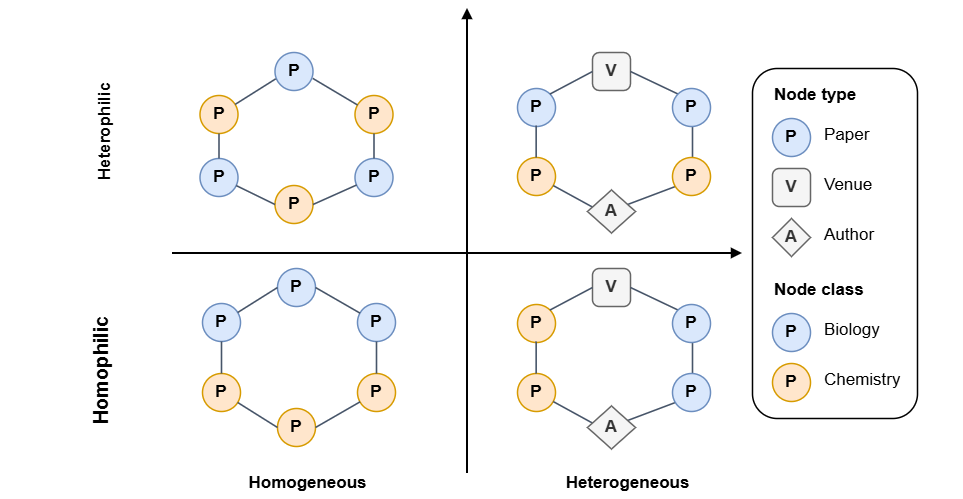
\includegraphics[width=\columnwidth]{figure/Het_HomGraph.drawio.png}
  \caption{An example of heterogeneous heterophilic graph. The graph contains multiple types of nodes and edges, and connected nodes may have different properties.}
  \label{fig:het_hom_graph}
\end{figure}

Many existing methods either focus on heterogeneous graphs but do not consider heterophily \cite{hu2020heterogeneous,mao2023hinormer,he2024spectral,yang2023simple,wang2019heterogeneous,zhang2019heterogeneous} or focus on heterophilic graphs but do not consider heterogeneous graphs \cite{grover2025spectro, yue2025graph,bodnar2022neural,ribeiro2026cooperative}. Recently, several research efforts have targeted heterogeneous heterophilic graphs and captured heterophily by using several approaches, such as using meta-paths to construct latent subgraphs suitable for learning heterophily and heterogeneity \cite{lu2026addressing,chen2025adaptive,li2025hetero2net,guo2023homophily,shen2025heterophily,wang2025homophily}, graph rewiring across node types \cite{tao2025cross}, using transformers directly in heterogeneous graphs \cite{lin2025heterophily}, or learnable mappings in heterogeneous graphs \cite{braithwaite2024heterogeneous}.

Moreover, meta-paths provide a natural way to describe composite relations in heterogeneous graphs. A
meta-path is a typed sequence of relations, such as a co-authorship relation, which means that in the graph the connection will be author-paper-author, that connects two authors
through a shared author and therefore expresses information that is not contained in either
endpoint alone \cite{sun2011pathsim} as shown in Figure \ref{fig:meta_path}. Existing heterogeneous heterophilic graph neural networks use meta-path sequences to construct
a node-to-node view, a filtered, or edited edge set for message passing
\cite{lu2026addressing,chen2025adaptive,li2025hetero2net,guo2023homophily,shen2025heterophily,wang2025homophily}.
This preserves the composite relation between the endpoints, but the concrete path
instance is no longer represented after the induced neighborhood has been formed. In the example
above, the path determines which papers may exchange information, while the two paper-author
relations inside that path do not remain as a joint structure that can directly shape propagation.
This loss matters specifically because of heterophily: whether two endpoints of a meta-path should
be treated as agreeing or disagreeing depends on the relation types along the path connecting them,
and once those relations are compressed into a single node-to-node edge, the model has no way to
condition propagation on that typed, heterogeneous evidence.

\begin{figure}
  \centering
  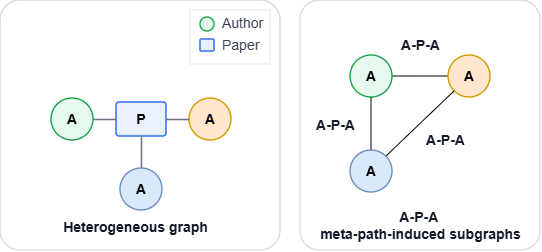
\includegraphics[width=\columnwidth]{figure/meta_path.drawio.png}
  \caption{Illustration of meta-path-based graph transformation. The original heterogeneous graph contains author and paper nodes connected by authorship relations. Under the A-P-A meta-path, two authors are connected when they share a common paper, producing an author-level meta-path-induced subgraph.}
  \label{fig:meta_path}
\end{figure}

Manual meta-path specification creates a second bottleneck. Relying on hand-crafted meta-paths from domain knowledge may be difficult in a complex network, and some useful paths might be ignored \cite{zhong2022pmhgnn,li2024lmsps}. Moreover, real-life datasets might not have predefined meta-paths.
HAN and MAGNN operate on predefined meta-path views \cite{wang2019han,fu2020magnn}. Automatic
methods reduce this burden through progressive sampling \cite{li2024lmsps}, searching algorithm \cite{zhang2026mctshgnn,li2023pmmm,li2026amphgnas,sun2025hgsearch}, or reinforcement learning
\cite{zhong2022pmhgnn}.
Although automatic meta-path search reduces reliance on expert knowledge, existing methods usually select or weight meta-paths only at the schema level. This is too coarse because concrete instances of the same schema are not equally informative. For example, a \texttt{PAP} schema may be useful overall, while some \texttt{PAP} instances connect unrelated papers and introduce misleading information. A schema-level method must either retain these noisy instances together with the useful ones or discard the entire schema. Moreover, many search methods first select a discrete set of schemas and then train the prediction model, preventing schema selection and instance relevance from being refined jointly by the task objective.

To address these problems, we propose
\method{}, a heterogeneous sheaf-Hodge framework that learns graph structures including meta-paths as higher-order supports. We first proposed defining a heterogeneous graph with meta-paths as a 2D-cellular graph, preserving graph structure and adding meta-paths directly into the graph. Our proposed framework learns based on sheaf theory, assigning a local vector space for each node, edge, and meta-path (face). The information will be translated between nodes, edges, and meta-paths through learned restriction maps. With diffusion over the sheaf-Hodge operators on the restriction maps, those nodes, edges, and meta-paths will be updated and learned jointly while allowing local-to-global consistency across the graph, resulting in a learned graph structure that preserves locality without breaking heterophily on heterogeneous graphs.

We further introduce \ampss{}, a two-stage schema-to-cell meta-paths selection mechanism that enumerates candidate meta-paths and jointly learns soft weights
for candidate schemas and their individual path instances. The schema weights identify useful
types of relational patterns, while the instance weights determine which concrete occurrences
should contribute to the model. The selected instances allow their constituent edges to interact through
the upper edge Laplacian. In this way, \ampss{} determines both \emph{which relational patterns
matter} and \emph{which occurrences of those patterns are informative}, resulting in a set of useful meta-paths for our \method{} framework to learn the graph structure and diffusion over the graph.

Moreover, graph classification requires summarizing node and edge information into a single
graph-level representation. Conventional pooling, such as plain mean pooling over node embeddings,
ignores that \method{}'s restriction maps are orthogonal, so the pooled descriptor is not
guaranteed to be invariant to the local frame of each node or edge stalk and can reflect an
arbitrary choice of gauge rather than the underlying sheaf geometry. We therefore introduce
\sheafconvpool{}, a gauge-invariant readout that scores Gram descriptors of the node and edge sheaf
state with learned attention and pools their attention-weighted mean and covariance, remaining
exactly invariant to \method{}'s orthogonal restriction maps by construction (\S~\ref{sec:readouts}).

Together, the three components address a common objective at different stages of the pipeline:
\ampss{} selects the typed higher-order support, the sheaf-Hodge model learns diffusion over node
and edge ranks, and \sheafconvpool{} produces a gauge-invariant graph-level summary of that
diffusion when a graph-level prediction is required.

The contributions of this work are as follows.
\begin{enumerate}
  \item We introduce \method{}, a heterogeneous sheaf-Hodge framework that retains concrete typed
  path instances as a face-like component on our proposed 2D-cellular graphs, resulting in a learned graph structure that preserves locality without breaking heterophily on heterogeneous graphs.
  \item We propose \ampss{}, a two-stage schema-to-cell selection mechanism that combines
  training-only candidate preselection with differentiable schema- and instance-level refinement
  inside the upper edge Laplacian. This allows \method{} to learn which concrete occurrences
  of a schema are useful for the task.
  \item For graph classification, we introduce \sheafconvpool{}, a gauge-invariant readout that
  scores per-node and per-edge Gram descriptors with learned attention and pools their
  attention-weighted mean and covariance, producing a graph-level representation that is
  invariant to \method{}'s orthogonal restriction maps by construction.
\end{enumerate}

To this end, we evaluate the framework across node classification, graph classification, and
heterogeneous link prediction. As a result, \method{} achieves the best overall performance across all tasks including node classification, graph classification, and heterogeneous link prediction.


Many existing methods address either heterogeneous graphs but do not consider heterophily \cite{hu2020heterogeneous,mao2023hinormer,he2024spectral,yang2023simple,wang2019heterogeneous,zhang2019heterogeneous} or focus on heterophilic graphs but do not consider heterogeneous graphs \cite{grover2025spectro, yue2025graph,bodnar2022neural,ribeiro2026cooperative}. Recently, several research efforts have targeted heterogeneous heterophilic graphs and model them through, such as using meta-paths to construct latent and informative subgraphs \cite{lu2026addressing,chen2025adaptive,li2025hetero2net,guo2023homophily,shen2025heterophily,wang2025homophily}, graph rewiring \cite{tao2025cross}, transformers model \cite{lin2025heterophily}, or sheaf-based model \cite{braithwaite2024heterogeneous}.

Moreover, meta-paths provide a natural way to expresses information that is not contained in either
endpoint alone \cite{sun2011pathsim}. For instances, a \texttt{Author-Paper-Author} meta-path describes a co-authorship relation in citation networks, as shown in Figure \ref{fig:meta_path}. Existing heterogeneous heterophilic graph neural networks use meta-path sequences to construct a node-to-node view or filtered edge set for message passing
\cite{lu2026addressing,chen2025adaptive,li2025hetero2net,guo2023homophily,shen2025heterophily,wang2025homophily}.
Those models keep the endpoint connection but removes the actual typed path that created it. In an A-P-A meta-path, for example, two authors are connected through a shared paper, but that paper and the two authorship relations are no longer modeled as part of propagation. This is problematic under heterophily, because whether information should be reinforced or contrasted depends on the typed relations along the path, and this can break heterogeneous structure of the graph.

\subsection{Cellular sheaves and neural diffusion}

A cellular complex represents a structure using cells of different dimensions. Nodes are
$0$-cells, edges are $1$-cells, and surfaces bounded by edges are $2$-cells. A graph is therefore
a one-dimensional cellular complex, while adding faces produces a two-dimensional complex. We
write $\sigma\unlhd\tau$ when a lower-dimensional cell $\sigma$ is incident to a
higher-dimensional cell $\tau$.
A cellular sheaf $\cF$ equips this combinatorial structure with local vector spaces and maps
between them. It assigns a vector space, called a \emph{stalk}, $\cF(\sigma)$ to each cell
$\sigma$, together with a linear restriction map
$F_{\sigma\unlhd\tau}:\cF(\sigma)\rightarrow\cF(\tau)$ for every incident pair. These maps specify
how information stored on different cells is transported into a common space and must compose
consistently along chains of incident cells.
On a graph $G=(V,E)$, a cellular sheaf $\cF$
assigns a vector space, called a stalk, $\cF(v)$ to every node and $\cF(e)$ to every edge. For
each incident pair $v\unlhd e$, a linear restriction map
$F_{v\unlhd e}:\cF(v)\rightarrow\cF(e)$ transports the node representation into the shared edge
space. Node and edge assignments form the cochain spaces
\begin{equation}
  C^0(G,\cF)=\bigoplus_{v\in V}\cF(v),
  \qquad
  C^1(G,\cF)=\bigoplus_{e\in E}\cF(e).
\end{equation}

Given an oriented edge $e=(u\rightarrow v)$, the first coboundary operator
$\delta_0:C^0(G,\cF)\rightarrow C^1(G,\cF)$ measures disagreement between the transported endpoint
representations:
\begin{equation}
  (\delta_0x)_e
  =
  F_{v\unlhd e}x_v-F_{u\unlhd e}x_u.
  \label{eq:background-delta0}
\end{equation}
The corresponding sheaf Laplacian is
$L_0=\delta_0^{\transpose}\delta_0$, with energy
$x^{\transpose}L_0x=\lVert\delta_0x\rVert_2^2$. When all stalks are one-dimensional and all
restriction maps are identities, $L_0$ reduces to the ordinary graph Laplacian.

Neural Sheaf Diffusion learns the restriction maps from node features and uses the resulting
Laplacian to propagate information \cite{bodnar2022neural}. This allows connected nodes to be
transformed before comparison, which is useful when their raw features are dissimilar.
HetSheaf extends this mechanism to heterogeneous graphs by conditioning restriction maps on node
and relation types \cite{braithwaite2024heterogeneous}. However, these models define sheaf
structure only over observed node-edge incidences. In contrast, \method{} additionally retains
selected meta-path instances as face-like supports and learns edge-to-face maps, enabling
diffusion over an explicit edge cochain.


\section{Methodology}
\label{sec:method}

\subsection{Problem Formulation}
We consider a directed heterogeneous graph
\(G=(V,E,\phi,\psi,X^{\mathrm{raw}})\), where
\(X^{\mathrm{raw}}=\{x_v^{\mathrm{raw}}\}_{v\in V}\), and
\(\phi:V\rightarrow\mathcal{T}\) and \(\psi:E\rightarrow\mathcal{R}\) assign node and relation
types. A node \(v\) has a raw feature vector
\(x_v^{\mathrm{raw}}\in\R^{d_{\phi(v)}}\), so different node types may use different input dimensions. For
each $t\in\mathcal{T}$, let $V_t=\{v\in V:\phi(v)=t\}$. We make no homophily assumption:
adjacent nodes may have different labels or dissimilar features. Each heterogeneous graph has a set of meta-path schemas $\Sigma$.
A meta-path schema
$\sigma=(t_0,r_1,t_1,\ldots,r_\ell,t_\ell)$ specifies a valid typed relation sequence, whereas
$f=(v_0,e_1,v_1,\ldots,e_\ell,v_\ell)$ denotes one concrete instance satisfying
$\phi(v_i)=t_i$ and $\psi(e_i)=r_i$. Let $\Sigma$ be the schema pool supplied manually or selected
by \ampss{}, let $\mathcal{I}_\sigma$ be the instances of schema $\sigma$, and let
$\mathcal{I}_\Sigma=\bigcup_{\sigma\in\Sigma}\mathcal{I}_\sigma$. The model retains each
$f\in\mathcal{I}_\Sigma$ as a face-like support over its ordered path edges. Given $G$ and this
support, the shared learning problem is to infer node-to-edge and edge-to-face maps together with
node and edge cochains that serve the following task settings.

\subsection{Framework Overview}

We introduce \method{}, a Heterophilic Heterogeneous Sheaf-Hodge Neural Network for supervised graph neural networks. As illustrated in Figure~\ref{fig:pipeline}, \method{} is organized into four stages.  \emph{Data Input} prepares typed
features, relations, and training-only diagnostics.  \emph{\ampss{} Selection} constructs a compact schema pool and refines the
importance of its concrete instances.  \emph{\method{} Learning} uses the selected paths to learn
node-edge-face geometry and diffuse node and edge cochains.  Finally, a task-specific readout
predicts target-node labels, candidate links, or graph labels.  These tasks share the same encoder
and operators: node classification reads selected target nodes, link prediction scores pairs of
final node states, and graph classification summarizes each graph with \sheafconvpool{}.

\begin{figure*}[t]
  \centering
  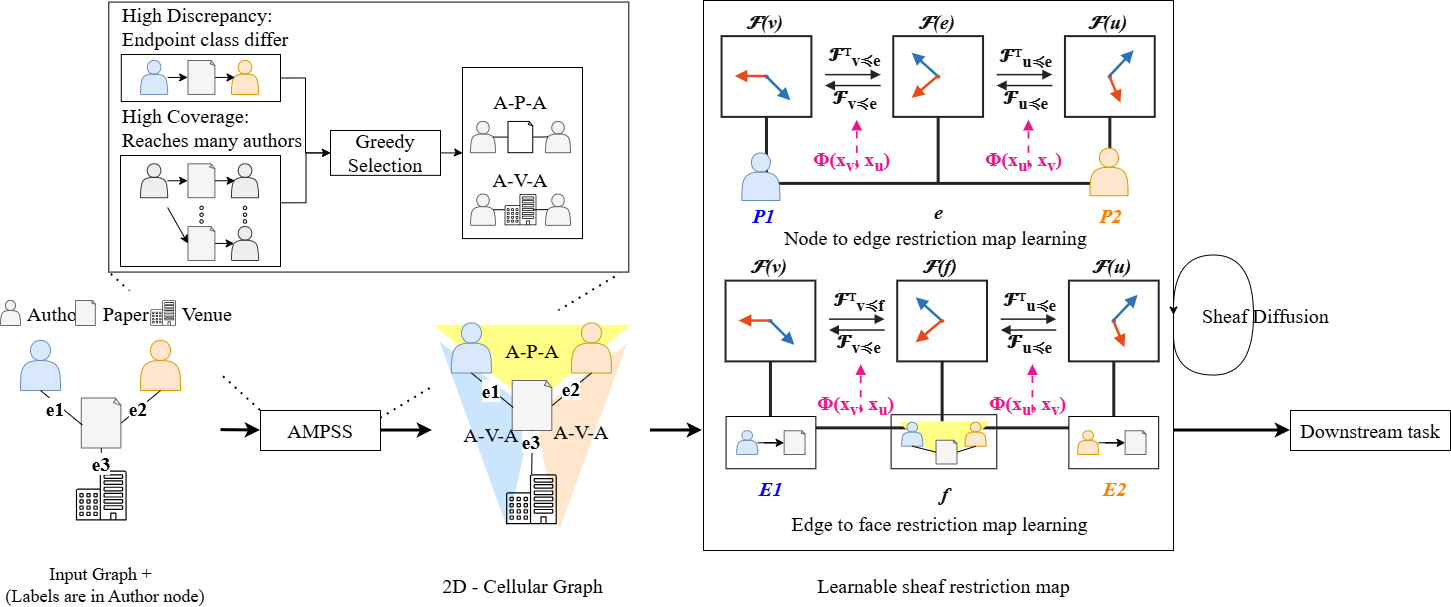
\includegraphics[width=\textwidth]{figure/h2snn_framework_overview.png}
  \caption{Overview of \method{}.  Typed graph data enter a training-only \ampss{} selection stage;
  selected schemas and weighted path instances then parameterize the node-edge-face geometry.
  Node and edge cochains diffuse in parallel before task-specific node, link, or graph prediction,
  with graph classification routed through \sheafconvpool{}.}
  \Description{A left-to-right four-stage diagram.  Data Input feeds AMPSS schema and instance
  selection, which feeds H2S-NN sheaf-Hodge geometry and parallel node and edge diffusion.  The
  output branches to node classification, link prediction, and graph classification through
  SheafConvPool.}
  \label{fig:pipeline}
\end{figure*}

\subsection{Task-Specific Data Preparation}

The data-input stage first flattens the heterogeneous graph into one node table and one directed
edge table while preserving node types, relation types, and the node-index range occupied by each
type.  Since raw feature dimensions may differ across node types, feature matrices are padded to a
common input width before they are passed to the neural encoder.  We write \(x_v\) below for this
preprocessed feature vector.

For node classification, the implementation also appends a compact relation-diagnostic vector to
each node feature.  This vector is computed from training labels only.  Starting from the labeled
training target nodes, a fixed label-propagation pass produces soft class distributions
\(\widehat y_v\) over all nodes; training labels are clamped during propagation, and validation and
test labels are never used.  For each relation type, the preprocessing then measures four
quantities: agreement between propagated labels at the two endpoints, agreement between simple
structural summaries such as degree and typed-path counts, agreement between feature-derived
summaries, and normalized mutual information between endpoint label distributions.  Stacking these
four values for every relation gives a global diagnostic vector \(m\in\R^{4|\mathcal{R}|}\), and
the node-classification input becomes
\begin{equation}
  x_v = x_v^{\mathrm{raw}}\concat m .
  \label{eq:feature-augmentation}
\end{equation}
Thus the node encoder receives both the original attributes and a training-only summary of how
different relation types behave in the graph.

The other tasks use the same flattened typed graph representation but adapt the diagnostics to the
available supervision.  For link prediction, there are no node class labels to append; instead,
\ampss{} builds a two-channel source/target role signal from training-positive edges only when it
scores link schemas.  The link-prediction encoder receives the raw padded node features.  For graph
classification, \ampss{} constructs its schema pool from training graphs in the current fold by
checking which typed path schemas occur differently across training classes.  Validation and test
graph labels do not enter this preprocessing.

\subsection{Typed Node-Edge Sheaf Construction}

This stage builds the node-to-edge geometry that jointly targets heterogeneity and heterophily:
type-specific encoders keep node types from sharing a vocabulary they were not designed to share,
and relation-conditioned restriction maps transport each edge's endpoints into a shared space
\emph{before} they are compared, so a large computed disagreement reflects the endpoints' typed,
relation-specific evidence rather than an assumption that connected nodes should already look
alike.

\paragraph{Type-specific node states.}
Different node types need not share a feature vocabulary or input dimension.  We therefore map
each type into the common stalk space before comparing adjacent nodes:
\begin{equation}
  h_v^{(0)}
  =\operatorname{Dropout}\!\left[
    \operatorname{GELU}\!\left(
      \operatorname{LN}(W_{\phi(v)}x_v+b_{\phi(v)})+q_{\phi(v)}
    \right)
  \right]\in\R^d ,
  \label{eq:node-encoder}
\end{equation}
where \(W_t,b_t\) are type-specific parameters and \(q_t\) is a learned type embedding.  A learned
node table supplies \(h_v^{(0)}\) when raw attributes are unavailable.  We initialize the diffused
node cochain as \(x^{(0)}=h^{(0)}\), and represent each relation \(r\) by
\(z_r\in\R^{d_r}\).

\paragraph{Relation-conditioned restrictions.}
An oriented edge \(e=(u\xrightarrow{r}v)\) must compare endpoints in a common edge stalk.  Two
relation-conditioned networks therefore infer
\(F_{u\unlhd e},F_{v\unlhd e}\in\R^{d\times d}\) from
\(h_u^{(0)}\), \(h_v^{(0)}\), and \(z_r\).  Each restriction is scaled orthogonal:
\begin{equation}
  F_{v\unlhd e}=\lambda_{v,e}Q_{v,e},
  \qquad Q_{v,e}^{\transpose}Q_{v,e}=I,
  \qquad \lambda_{v,e}>0 ,
  \label{eq:conformal-map}
\end{equation}
and analogously for \(F_{u\unlhd e}\).  The orthogonal factor aligns local coordinates, while the
positive scale adjusts the strength of the incidence.  These restrictions define the first
coboundary immediately:
\begin{equation}
  (\delta_0x)_e
  =F_{v\unlhd e}x_v-F_{u\unlhd e}x_u .
  \label{eq:delta0}
\end{equation}
Thus, \(\delta_0x\) measures relation-aware endpoint disagreement rather than raw feature
difference.

\paragraph{Independent edge initialization.}
Endpoint disagreement is informative, but it need not span every useful edge signal.  We initialize
the edge cochain with a separate network,
\begin{equation}
  s_e^{(0)}
  =\operatorname{MLP}_{\mathrm{init}}\!\left(
    h_u^{(0)}\concat h_v^{(0)}\concat z_r
    \concat(\delta_0h^{(0)})_e
  \right),
  \label{eq:edge-init}
\end{equation}
so \(s^{(0)}\neq\delta_0h^{(0)}\) in general.  This preserves an edge component outside
\(\operatorname{im}\delta_0\) for the subsequent lower- and upper-Hodge interactions.

\subsection{\ampss{}: Adaptive Meta-Path Schema-to-Cell Selection}
\label{sec:ampss}

\ampss{} separates economical structure search from task-driven refinement.  The first stage is a
non-differentiable, training-only construction of a candidate pool; the second stage learns soft
weights for the retained schemas and their concrete instances jointly with \method{}.

\paragraph{Stage I: candidate generation and preselection.}
The first stage constructs a small set of typed higher-order supports before the neural model is
trained.  It does so at the level of the heterogeneous schema rather than by immediately traversing
all concrete node paths.  We first form a directed type graph whose nodes are entity types and whose
directed edges are relation types, e.g., \(P\xrightarrow{\mathrm{writes}^{-1}}A\) and
\(A\xrightarrow{\mathrm{writes}}P\) in a paper--author network.  A bounded depth-first search over
this type graph enumerates valid schema candidates
\(\sigma=(t_0,r_1,t_1,\ldots,r_\ell,t_\ell)\) subject to the allowed length range and, when
required by the task, the start and end target types.  This step therefore proposes only type-valid
relational routes; it does not yet decide that any route is useful.

For each candidate schema, \ampss{} then samples concrete instances in the original graph.  Starting
from nodes of type \(t_0\), it follows the prescribed relation sequence
\((r_1,\ldots,r_\ell)\) and records paths
\(f=(v_0,e_1,v_1,\ldots,e_\ell,v_\ell)\) whose node and edge types match the schema.  Separate
budgets cap the number of candidate schemas, the number of instances expanded from one anchor node,
the number of instances retained for one schema, and the total number of materialized instances.
These caps make the construction economical while still exposing the model to the main typed
relational patterns present in the graph.

The preselection score is designed to keep schemas that are both informative and usable as
face-like supports.  For node classification, training labels are propagated for a fixed number of
steps to obtain soft endpoint distributions \(\widehat y_v\).  A concrete path receives a large
discrepancy when its two endpoints carry different training-derived class evidence, and a schema
receives the average discrepancy of its sampled instances:
\begin{equation}
  d(f)=\norm{\widehat y_{v_0}-\widehat y_{v_\ell}}_2^2,
  \qquad
  D(\sigma)=\frac{1}{|\mathcal{I}_{\sigma}|}
  \sum_{f\in\mathcal{I}_{\sigma}}d(f).
  \label{eq:discrepancy}
\end{equation}
Intuitively, this favors schemas whose endpoints expose nontrivial class contrast under the
training signal, which can create useful edge-level disagreement for the subsequent Hodge diffusion.
For link prediction, the same idea is implemented with two propagated endpoint-role channels that
mark source and target positions using training-positive edges only.  Neither validation nor test
labels or links contribute to these statistics.

For graph classification, endpoint discrepancy is not the relevant signal.  Let
\(n_{\sigma,c}^{\mathrm{pres}}\) be the number of training graphs of class \(c\) in which schema
\(\sigma\) occurs, \(N_c\) the number of training graphs in that class, and \(n_\sigma\) the total
number of its materialized instances.  The presence score is
\begin{equation}
  P_G(\sigma)
  =\operatorname{Var}_{c}\!\left(
    \frac{n_{\sigma,c}^{\mathrm{pres}}}{\max(N_c,1)}
  \right)+10^{-3}\log(1+n_\sigma).
  \label{eq:graph-presence-score}
\end{equation}
This favors schemas whose presence differs across training classes, with frequency used only as a
small tie breaker.

For node and link tasks, \ampss{} greedily builds the selected pool one schema at a time.  The
score combines four quantities.  The discrepancy \(D(\sigma)\) measures task relevance.  The
endpoint coverage \(C(\sigma)\) measures how many target-type endpoints are reached by the sampled
instances, so a schema that appears only in a tiny corner of the graph is not selected merely
because it has a high local score.  The type diversity \(V(\sigma)\) rewards schemas that pass
through multiple semantic types rather than repeatedly using the same type pattern.  Finally,
\(J(\sigma,\sigma')\) measures endpoint-set overlap with an already selected schema
\(\sigma'\), discouraging several selected schemas from describing nearly the same region of the
graph.  Given the current pool \(S\), the greedy score is
\begin{equation}
  q(\sigma\mid S)=
  \frac{D(\sigma)^{a_d}C(\sigma)^{a_c}V(\sigma)^{a_v}}
       {1+\max_{\sigma'\in S}J(\sigma,\sigma')} ,
  \label{eq:topology-score}
\end{equation}
The numerator prefers schemas that are informative, sufficiently covered, and semantically varied;
the denominator lowers the priority of schemas that are redundant with the pool already chosen.
Graph tasks use the class-presence score \(P_G(\sigma)\) instead of Equation~\ref{eq:topology-score}.
After this greedy pass, the selected schemas are materialized as ordered path supports, together
with the closure pairs used by the node-side correction.  This entire stage fixes the candidate
support and is intentionally non-differentiable; the next stage decides how strongly the retained
schemas and their individual instances should participate in the learned operator.

\paragraph{Stage II: differentiable schema and instance refinement.}
Preselection decides what can be considered; it does not force every retained structure to
contribute equally.  We learn one gate per schema and a state-dependent gate for every path
instance:
\begin{equation}
  \begin{aligned}
  \alpha_\sigma&=\operatorname{sigmoid}(\theta_\sigma),\\
  \beta_f&=\operatorname{sigmoid}\!\left(
    g_\beta(h_{v_0}^{(0)}\concat h_{v_\ell}^{(0)}\concat e_\sigma)
  \right),\\
  w_f&=\alpha_{\sigma(f)}\beta_f .
  \end{aligned}
  \label{eq:gates}
\end{equation}
Here \(e_\sigma\) is a learned schema embedding.  Schema logits are warm-started from standardized
preselection scores, while \(\beta_f\) lets two instances of the same schema have different
effects.  During training, partial-schema propagation retains each schema with probability
\(p_{\mathrm{keep}}\) and rescales a retained gate by \(1/p_{\mathrm{keep}}\), following the
stabilization idea of partial message propagation \cite{li2023pmmm}.

The discovery loss applies complementary pressures rather than a single hard selection rule:
\begin{equation}
  \begin{aligned}
  \cL_{\mathrm{disc}}={}&
  \lambda_s\cL_{\mathrm{sparse\text{-}schema}}
  +\lambda_i\cL_{\mathrm{sparse\text{-}instance}}
  +\lambda_r\cL_{\mathrm{redundancy}}\\
  &+\lambda_v\cL_{\mathrm{coverage}}
  +\lambda_{\mathrm{cost}}\cL_{\mathrm{cost}}
  +\lambda_H\cL_{\mathrm{entropy}} .
  \end{aligned}
  \label{eq:discovery-loss}
\end{equation}
Schema and instance terms discourage diffuse activation; redundancy penalizes similar active
coverage profiles; the negative coverage reward discourages a trivial empty pool; cost suppresses
long, frequently instantiated schemas; and entropy minimization sharpens schema decisions.  These
terms refine only the preselected pool and do not make candidate generation differentiable.

\begin{algorithm}[t]
  \caption{\ampss{} candidate preselection and differentiable refinement}
  \label{alg:ampss}
  \begin{algorithmic}[1]
    \REQUIRE Typed relation graph, training split, schema and instance budgets
    \STATE \textbf{Stage I: Candidate generation and training-only preselection}
    \STATE Enumerate bounded typed schemas and sample concrete instances
    \STATE Compute node/link discrepancy scores or graph presence scores
    \STATE Greedily retain a compact pool \(\Sigma\) and materialize its path supports
    \STATE Initialize \(\theta_\sigma\) from standardized preselection scores
    \FOR{each training epoch}
      \STATE \textbf{Stage II: Differentiable schema and instance refinement}
      \STATE Use uniform face weights during warm-up
      \STATE Compute \(\alpha_\sigma\), \(\beta_f\), and \(w_f=\alpha_{\sigma(f)}\beta_f\)
      \STATE Apply partial-schema propagation with keep probability \(p_{\mathrm{keep}}\)
      \STATE Run matrix-free sheaf-Hodge diffusion and the task readout
      \STATE Optimize Equation~\ref{eq:loss}
    \ENDFOR
  \end{algorithmic}
\end{algorithm}

\subsection{Path-Supported Edge-Face Geometry}
\label{sec:face-geometry}

Consider a selected \(P\!-\!A\!-\!P\) instance
\(f=(v_0,e_1,v_1,e_2,v_2)\).  The model retains the ordered path edges
\(\partial_{\mathrm{path}}f=(e_1,e_2)\) as the path part of the boundary: it does not replace the instance by
a shortcut edge between its endpoint papers.  For a general instance
\(f=(v_0,e_1,v_1,\ldots,e_\ell,v_\ell)\), an edge token combines its endpoint states and relation,
\begin{equation}
  \begin{aligned}
  g_i&=\operatorname{MLP}_g\!\left(
    h_{v_{i-1}}^{(0)}\concat h_{v_i}^{(0)}\concat z_{\psi(e_i)}
  \right),\\
  (o_1,\ldots,o_\ell)&=\operatorname{LSTM}(g_1,\ldots,g_\ell).
  \end{aligned}
\end{equation}
The ordered encoder distinguishes positions along the path.  Attention then pools the sequence into
a single summary, which produces one free map per instance:
\begin{equation}
  \pi_{fi}
  =\operatorname{softmax}_{i}\!\left(
    \frac{o_i^{\transpose}a}{\sqrt{d_h}}
  \right),
  \qquad
  A_f
  =\operatorname{reshape}\!\Big(W_F\textstyle\sum_i\pi_{fi}o_i+b_F,\,d,d\Big).
  \label{eq:face-map}
\end{equation}
Attention shapes \(A_f\); it deliberately does not rescale individual edges' maps, because a
non-uniform per-edge factor would destroy the boundary cancellation established below.

The per-edge maps are then \emph{not} emitted independently.  A cellular sheaf is a functor on the
face poset, so an edge-to-face map must compose with the node-to-edge maps beneath it; emitting both
from separate networks breaks that functoriality, and with it the cochain property.  We therefore
carry a transport to the base vertex \(v_0\) along the boundary:
\begin{equation}
  \begin{aligned}
  T_{v_0}&=A_f,
  \qquad
  T_{v_i}=T_{v_{i-1}}F_{u\unlhd e_i}^{-1}F_{v\unlhd e_i},\\
  F_{e_i\unlhd f}&=T_{v_{i-1}}F_{u\unlhd e_i}^{-1},
  \end{aligned}
  \label{eq:transport}
\end{equation}
where \(u=v_{i-1}\) and \(v=v_i\) are the endpoints of \(e_i\).  The inverse is available in closed
form: by Eq.~\eqref{eq:conformal-map} each map is a positive scale times an orthogonal factor, so
\(F^{-1}=F^{\transpose}/\lambda^2\), and no linear solve is required.  Each map
\(F_{e_i\unlhd f}:\cF(e_i)\rightarrow\cF(f)\) still transports the \(i\)-th edge state into the
shared face stalk, and still varies per instance and per relation; what changes is that a single
\(d\times d\) matrix per instance is learned freely rather than \(\ell\) of them.

Let \(\eta(e,f)\in\{-1,+1\}\) be the stored incidence orientation.  The face gate enters the
weighted second coboundary:
\begin{equation}
  (\delta_{1,w}s)_f
  =\sqrt{w_f}\sum_{e\in\partial f}
    \eta(e,f)F_{e\unlhd f}s_e .
  \label{eq:delta1}
\end{equation}
Writing
\(B_fs=\sum_{e\in\partial f}\eta(e,f)F_{e\unlhd f}s_e\), its upper-Hodge
contribution is therefore
\begin{equation}
  \delta_{1,w}^{\transpose}\delta_{1,w}
  =\sum_{\sigma\in\Sigma}\sum_{f\in\mathcal{I}_{\sigma}}
    w_f B_f^{\transpose}B_f .
  \label{eq:weighted-up}
\end{equation}
The square root is important: it makes each face contribute linearly in \(w_f\), not quadratically.

An open path is not the boundary of a \(2\)-cell: a cell is attached along a cycle.  Each instance
therefore also carries a synthetic closure \(1\)-cell \(e_{\mathrm{cl}}=(v_\ell\rightarrow v_0)\),
oriented along the cycle, which completes \(\partial f=(e_1,\ldots,e_\ell,e_{\mathrm{cl}})\).  It is a
stateful edge with its own stalk, and its restriction maps are \emph{defined} rather than learned:
\begin{equation}
  F_{v_0\unlhd e_{\mathrm{cl}}}=I,
  \qquad
  F_{v_\ell\unlhd e_{\mathrm{cl}}}=T_{v_0}^{-1}T_{v_\ell},
  \qquad
  F_{e_{\mathrm{cl}}\unlhd f}=A_f .
  \label{eq:closure-maps}
\end{equation}
The middle map reduces to \(\prod_i F_{u\unlhd e_i}^{-1}F_{v\unlhd e_i}\), the holonomy of the path
itself: it is independent of \(A_f\) and adds no parameters.  The closure cell is thus a bookkeeping
device that makes ``traverse this path and return'' well posed, not an asserted relation between the
endpoints.  Figure~\ref{fig:sheaf-hodge-operator} makes this boundary explicit.

\begin{proposition}[Exact cochain condition]
\label{prop:chain}
For every instance whose node sequence is a simple path, the maps of
Eqs.~\eqref{eq:transport}--\eqref{eq:closure-maps} satisfy
\(\delta_{1,w}\delta_0=0\) identically, for every node cochain and every value of the learned
parameters, with no assumption that the sheaf has trivial holonomy.
\end{proposition}

\begin{proof}
By construction \(F_{e_i\unlhd f}F_{u\unlhd e_i}=T_{v_{i-1}}\) and
\(F_{e_i\unlhd f}F_{v\unlhd e_i}=T_{v_i}\), so the \(i\)-th boundary term of \(\delta_{1,w}\delta_0x\)
equals \(T_{v_i}x_{v_i}-T_{v_{i-1}}x_{v_{i-1}}\), and summing over the path telescopes to
\(T_{v_\ell}x_{v_\ell}-T_{v_0}x_{v_0}\).  Eq.~\eqref{eq:closure-maps} gives
\(F_{e_{\mathrm{cl}}\unlhd f}F_{v_0\unlhd e_{\mathrm{cl}}}=T_{v_0}\) and
\(F_{e_{\mathrm{cl}}\unlhd f}F_{v_\ell\unlhd e_{\mathrm{cl}}}=T_{v_\ell}\), so the closure term
contributes \(T_{v_0}x_{v_0}-T_{v_\ell}x_{v_\ell}\) and the total vanishes.  Simplicity is required
because the transport assigns one map per node position; a revisited node — including a coincident
endpoint pair — would be assigned two values.
\end{proof}

\noindent Empirically the residual \(\norm{\delta_{1,w}\delta_0h^{(0)}}/\norm{\delta_0h^{(0)}}\) is
at the level of single-precision roundoff (\(\sim\!10^{-7}\)) on all evaluated datasets, for both
manual and \ampss{} schema sets.

\begin{figure}[t]
  \centering
  \fbox{\rule{0pt}{4.2cm}\rule{0.94\columnwidth}{0pt}}
  %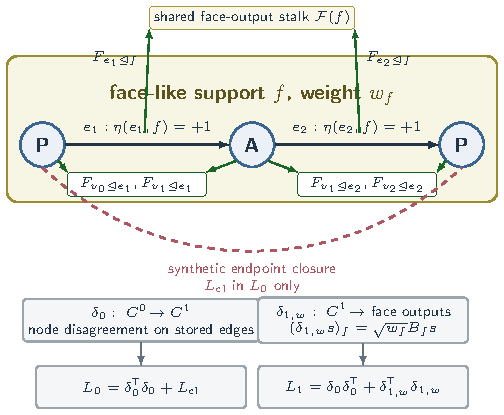
\includegraphics[width=\columnwidth]{figure/h2snn_sheaf_hodge_operator.pdf}
  \caption{AMPSS-selected path instances define a sheaf-Hodge operator. Currently in construction.}
  \label{fig:sheaf-hodge-operator}
\end{figure}

\subsection{Matrix-Free Sheaf-Hodge Diffusion}
\label{sec:closure}

The two coboundaries induce one node operator and one edge operator:
\begin{align}
  L_0x
  &=\delta_0^{\transpose}\delta_0x,
  \label{eq:l0}\\
  L_1s
  &=\underbrace{\delta_0\delta_0^{\transpose}s}_{\text{lower edge term}}
    +\underbrace{\delta_{1,w}^{\transpose}\delta_{1,w}s}_{\text{upper edge term}} .
  \label{eq:l1}
\end{align}
The lower edge term compares edge signals through their incident nodes; the upper term couples the
edges of a boundary cycle through their shared face.  Because the closure \(1\)-cell of
Section~\ref{sec:face-geometry} is an ordinary member of the edge set, it enters \(\delta_0\) — and hence
\(L_0\) and the lower edge term — exactly like a data edge; no separate node-side correction is
applied.  Its restriction maps are the path holonomy of Eq.~\eqref{eq:transport}, so it introduces
no parameters of its own, and a scale \(\gamma>0\) on them is absorbed by the compensating factor in
\(F_{e_{\mathrm{cl}}\lhd f}\), leaving Proposition~\ref{prop:chain} unaffected while tuning how
strongly the boundary cycle closes at the node level.

Starting from \(x^{(0)}=h^{(0)}\) and the independent \(s^{(0)}\), \(K\) explicit Euler steps give
\begin{equation}
  \begin{aligned}
  x^{(k+1)}&=x^{(k)}-\eta_0L_0x^{(k)},\\
  s^{(k+1)}&=s^{(k)}-\eta_1L_1s^{(k)},
  \qquad k=0,\ldots,K-1 .
  \end{aligned}
  \label{eq:diffusion}
\end{equation}
The positive step sizes may be learned.  Node and edge cochains evolve in parallel under geometry
inferred from the same initial node states; there is no cross-rank recurrence between Euler steps.
Layer normalization yields the terminal states \(x^\star\) and \(s^\star\).

Execution is matrix-free: the model applies restrictions in batches and aggregates incident
contributions, without materializing global \(Nd\times Nd\) or \(Md\times Md\) matrices.  Three
implementation boundaries remain consequential.  First, \(\delta_{1,w}\) spans the complete boundary
cycle: the \(\ell\) path edges together with the closure \(1\)-cell.  Second, signed incidences are
supported, and the uniform \(+1\) used here is the correct boundary map precisely because
enumeration traverses every edge along its stored direction and stores the closure cell oriented
along the cycle; the pipeline asserts this rather than assuming it, so a future change to reverse
traversal fails loudly instead of silently invalidating the signs.  Third, because faces must be
simple paths for the transport of Eq.~\eqref{eq:transport} to be well defined, instances that revisit
a node — including those whose endpoints coincide — are excluded during enumeration.  On the
manual meta-path templates this removes a negligible fraction of instances, since the search
backfills its per-anchor budget with simple paths.  Unlike earlier path-supported sheaf
constructions, \(\delta_{1,w}\delta_0=0\) is not encouraged by a penalty but holds identically
(Proposition~\ref{prop:chain}).

\subsection{Downstream Readouts}
\label{sec:readouts}

\paragraph{Node classification.}
Let
\(\bar s_v^\star=|E(v)|^{-1}\sum_{e\ni v}s_e^\star\), with a zero vector for an isolated node.
The target-node classifier retains the terminal node state, the pre-diffusion state, and the local
edge summary:
\begin{equation}
  \widehat y_v
  =\operatorname{MLP}_{\mathrm{node}}\!\left(
    x_v^\star\concat h_v^{(0)}\concat\bar s_v^\star
  \right).
  \label{eq:node-readout}
\end{equation}
The third view gives the supervised node head direct access to information transformed by the
upper edge operator.

\paragraph{Link prediction.}
Candidate endpoints are decoded from their final node states using a dot product, a
relation-conditioned DistMult decoder, or a concatenation MLP.  The current link head does not
directly consume \(s^\star\); consequently, its task loss reaches the upper-edge pathway only
through shared training terms, not through an edge-state link decoder.

\paragraph{Graph classification.}
A graph head must be invariant under node and edge permutations and orthogonal stalk gauges.
\sheafconvpool{} meets these requirements while retaining both terminal and initial node views and
the learned edge cochain.  It is a single-level terminal readout.

\subsection{\sheafconvpool{}}

For each node \(v\), \sheafconvpool{} stacks three aligned views,
\begin{equation}
  Z_v^{(0)}
  =\begin{bmatrix}x_v^\star&h_v^{(0)}&\bar s_v^\star\end{bmatrix}
  \in\R^{d\times3}.
\end{equation}
For each stored edge \(e\), it similarly forms
\begin{equation}
  Z_e^{(1)}
  =\begin{bmatrix}
    (\delta_0x^\star)_e&(\delta_0h^{(0)})_e&s_e^\star
  \end{bmatrix}
  \in\R^{d\times3}.
\end{equation}
The corresponding \(3\times3\) Gram descriptors are
\(G_i^{(r)}=(Z_i^{(r)})^{\transpose}Z_i^{(r)}\), for rank \(r\in\{0,1\}\).
Under an orthogonal local gauge \(Z_i^{(r)}\mapsto Q_iZ_i^{(r)}\),
\(G_i^{(r)}\) is unchanged.  The readout therefore learns only from coordinate-independent
inner products among its three views.

Separate node and edge networks project the flattened descriptors,
\(u_i^{(r)}=\rho_r(\operatorname{vec}G_i^{(r)})\in\R^{d_p}\), and score them with invariant
attention.  Within each graph and rank,
\begin{equation}
  a_i^{(r)}
  =\frac{\exp(g_r(u_i^{(r)}))}
         {\sum_{j\in\mathcal{C}_r}\exp(g_r(u_j^{(r)}))},
  \qquad
  \mu_r=\sum_{i\in\mathcal{C}_r}a_i^{(r)}u_i^{(r)},
\end{equation}
where \(\mathcal{C}_0\) and \(\mathcal{C}_1\) are the graph's nodes and edges.  A mean alone cannot
record whether informative descriptors are concentrated or dispersed, so the readout also computes
\begin{equation}
  \Sigma_r
  =\sum_{i\in\mathcal{C}_r}a_i^{(r)}
    (u_i^{(r)}-\mu_r)(u_i^{(r)}-\mu_r)^{\transpose}.
\end{equation}
The graph representation concatenates
\(\mu_0\), the upper triangle of \(\Sigma_0\), \(\mu_1\), and the upper triangle of
\(\Sigma_1\); an MLP maps this vector to graph logits.  Softmax normalization and moment summation
make the construction permutation invariant, while the Gram descriptors make it invariant under
the model's orthogonal stalk gauges.

\begin{figure}[t]
  \centering
  \fbox{\rule{0pt}{4.2cm}\rule{0.94\columnwidth}{0pt}}
  %\includegraphics[width=\columnwidth]{figure/sheafconvpool_architecture.pdf}
  \caption{\sheafconvpool{} graph readout.  Node and edge view stacks become orthogonal-gauge
  invariant through \(Z^{\transpose}Z\).  Separate projections and invariant attention produce
  weighted means and covariances; their node/edge summaries are concatenated for graph
  classification. The actual picture is currently in construction.}
  \Description{Two parallel node and edge branches.  Each starts with three stalk-valued views,
  forms a Gram descriptor, applies a learned projection and invariant attention, and computes a
  weighted mean and covariance.  Upper-triangular covariance vectors join the means, and the two
  branches concatenate before an MLP outputs graph logits.}
  \label{fig:sheafconvpool}
\end{figure}

\subsection{Training Objective}

The geometry carries no auxiliary loss.  The task term is cross-entropy for single-label node and
graph classification, binary cross-entropy for multi-label classification and link prediction, with
the appropriate training mask or sampled training pairs, and the only additional term is the
\ampss{} schema-selection objective:
\begin{equation}
  \cL
  =\cL_{\mathrm{task}}
   +\rho(t)\cL_{\mathrm{disc}} .
  \label{eq:loss}
\end{equation}
During discovery warm-up, gates are bypassed by uniform face weights and \(\rho(t)=0\).  After
warm-up, the schema and instance gates activate; \(\rho(t)\) is either applied at full strength or
annealed linearly to one over a configured interval.  This schedule lets task gradients establish a
useful path geometry before sparsity, redundancy, and cost pressures dominate.  For manual schema
sets \(\cL_{\mathrm{disc}}\) is absent and the objective reduces to the task loss alone.

That the geometric terms are absent is a consequence of the construction, not an omission.  A chain
penalty is unnecessary because Proposition~\ref{prop:chain} makes \(\delta_{1,w}\delta_0\) vanish
identically; on an open path such a penalty is in any case unsatisfiable except by degenerate face
maps, since the two endpoint blocks of \(\delta_{1,w}\delta_0\) each appear in a single term while the
node-to-edge maps are invertible.  A consistency penalty \(\norm{s^\star-\delta_0x^\star}^2\) is
counterproductive: \(x\) evolves under \(L_0\) alone and the edge channel never feeds back into it, so
driving \(s^\star\) to \(\delta_0x^\star\) would make the edge cochain a deterministic image of the
node cochain and the faces would contribute nothing.  A face-level Dirichlet penalty
\(\norm{\delta_{1,w}s^\star}^2\) is counterproductive for the same reason at one rank higher: with the
cochain condition exact, \(\delta_{1,w}s^\star\) is precisely the curl component of the edge cochain
and the only part the upper Hodge term \(\delta_{1,w}^{\transpose}\delta_{1,w}\) acts on, so shrinking
it drives the face branch inert.  The edge cochain is therefore left free at both ranks.



//Night
\documentclass[sigconf,anonymous,review]{acmart}

\usepackage{amsthm}
\usepackage{algorithm}
\usepackage{algorithmic}
\usepackage{multirow}

\AtBeginDocument{%
  \providecommand\BibTeX{{Bib\TeX}}}

% Replace the ACM metadata below with the values supplied by the proceedings venue.
\setcopyright{acmlicensed}
\copyrightyear{2026}
\acmYear{2026}
\acmDOI{XXXXXXX.XXXXXXX}
\acmConference[Conference acronym 'XX]{ACM Conference}{Month DD-DD, 2026}{City, Country}
\acmISBN{978-1-4503-XXXX-X/2026/MM}

\newcommand{\R}{\mathbb{R}}
\newcommand{\method}{\textsc{H2S-NN}}
\newcommand{\ampss}{\textsc{AMPSS}}
\newcommand{\sheafconvpool}{\textsc{SheafConvPool}}
\newcommand{\cF}{\mathcal{F}}
\newcommand{\cL}{\mathcal{L}}
\newcommand{\norm}[1]{\left\lVert #1\right\rVert}
\newcommand{\transpose}{\mathsf{T}}
\newcommand{\concat}{\mathbin\Vert}
\newtheorem{proposition}{Proposition}

\title[H2S-NN]{H2S-NN: Heterophilic Heterogeneous Neural Networks with Adaptive Meta-Path Selection}

% Replace the affiliation placeholder before submission.
\author{Peeradon Sarnkaew}
\email{peeradonsarnkaew46@gmail.com}
\affiliation{%
  \institution{Independent Researcher}
  \city{Bangkok}
  \country{Thailand}
}
\renewcommand{\shortauthors}{Sarnkaew}

\begin{document}

\begin{abstract}
Heterogeneous graphs contain many node and relation types, and learning on them raises two problems that are usually handled separately but really occur together. Different relation types carry different meanings, so a single shared update rule can blur information that should stay type-aware; and many of these relations are heterophilic, where connected nodes need not share a label or similar features, so a model that assumes neighbors agree can discard the very signal a relation carries. Meta-paths, typed relations such as author-paper-author, are the standard way to expose multi-hop semantics, but existing methods collapse each into a node-to-node view and lose the path structure a heterophily-aware model could act on. We introduce \method{}, which keeps both problems in view. It compares each edge's endpoints in a shared space, so that a relation-aware disagreement rather than a raw feature gap drives learning, and it retains selected meta-path instances as higher-order structure instead of reducing them to endpoint pairs. To avoid hand-picking meta-paths, \ampss{} learns which schemas and instances matter jointly with the task, while \sheafconvpool{} pools the result for graph classification. Across benchmarks, \method{} leads on node and graph classification and stays competitive on link prediction; ablations confirm that each component contributes.
\end{abstract}

\ccsdesc[500]{Computing methodologies~Neural networks}

\keywords{heterogeneous graph neural networks, heterophily, sheaf neural networks, meta-path discovery, graph pooling}

\maketitle

\section{Introduction}
\label{sec:introduction}


Heterogeneous graphs are a common representation for modeling complex relational structures, such as citation 
networks \cite{liu2014meta} or social interactions \cite{singh2025overview}. Unlike homogeneous graphs, heterogeneous graphs contain multiple types of nodes and edges wwith distinct semantic roles \cite{sun2013mining}. Moreover, many graphs are also heterophilic, where nodes may have different properties. A graph can therefore be both heterogeneous and heterophilic, resulting in a much more complex learning task called heterogeneous heterophilic graph learning, as shown in Figure \ref{fig:het_hom_graph}. Furthermore, modeling graphs under the simplifying assumptions of homogeneity or homophily can obscure important structural and relational patterns. This mismatch provides the model with an incomplete representation of the original graph and may consequently degrade predictive performance \cite{lin2025heterophily}. 

\begin{figure}
  \centering
  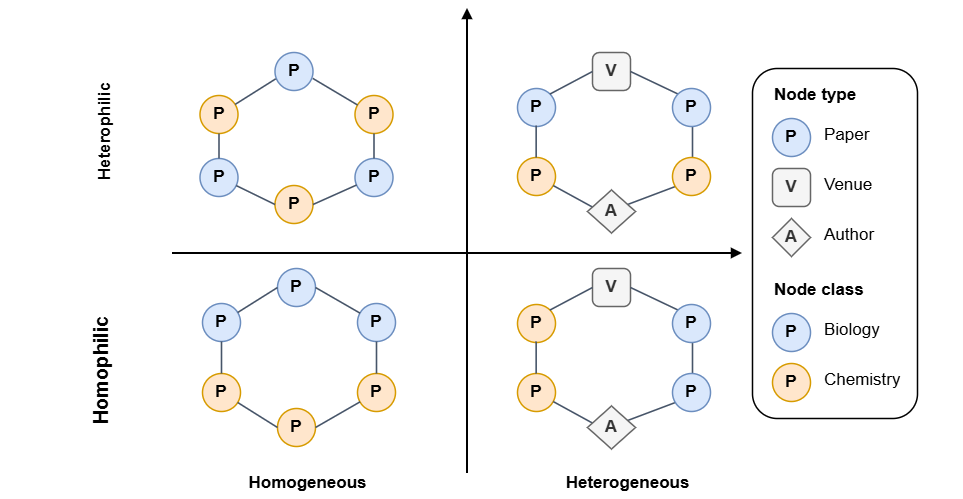
\includegraphics[width=\columnwidth]{figure/Het_HomGraph.drawio.png}
  \caption{An example of heterogeneous heterophilic graph. The graph contains multiple types of nodes and edges, and connected nodes may have different properties.}
  \label{fig:het_hom_graph}
\end{figure}

Many existing methods address either heterogeneous graphs without explicitly considering heterophily \cite{hu2020heterogeneous,mao2023hinormer,he2024spectral,yang2023simple,wang2019heterogeneous,zhang2019heterogeneous} or heterophilic graphs without modeling heterogeneous node and edge types \cite{grover2025spectro,yue2025graph,bodnar2022neural,ribeiro2026cooperative}. Recent methods have begun to address heterogeneous heterophilic graphs through meta-path-based latent subgraphs \cite{lu2026addressing,chen2025adaptive,li2025hetero2net,guo2023homophily,shen2025heterophily,wang2025homophily}, graph rewiring \cite{tao2025cross}, graph transformers \cite{lin2025heterophily}, and sheaf-based mappings \cite{braithwaite2024heterogeneous}. Among these directions, meta-paths can express information that is not contained in either endpoint alone \cite{sun2011pathsim}. For instance, an \texttt{Author-Paper-Author} meta-path describes a co-authorship relation in citation networks, as shown in Figure~\ref{fig:meta_path}. However, existing methods either ignore meta-paths completely, use meta-paths as semantic views, filtered edge sets, or aggregation channels rather than retaining each concrete path instance as part of the propagation structure. For example, an \texttt{A-P-A} meta-path can connect two authors through a shared paper, but after it is converted into an author-author view, the shared paper and the two authorship edges no longer directly shape the propagation operator. This is limiting under heterophily, because whether information should be reinforced or contrasted can depend on the relations along the path, not only on the endpoint connection. This can weaken locality and higher-order information from meta-paths as a part of graph structure.

\begin{figure}
  \centering
  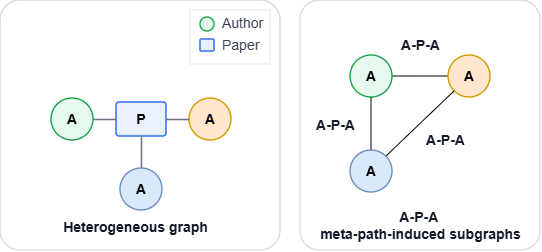
\includegraphics[width=\columnwidth]{figure/meta_path.drawio.png}
  \caption{Illustration of meta-path-based graph transformation. The original heterogeneous graph contains author and paper nodes connected by authorship relations. Under the A-P-A meta-path, two authors are connected when they share a common paper, producing an author-level meta-path-induced subgraph.}
  \label{fig:meta_path}
\end{figure}

Manual meta-path specification creates a second bottleneck. Hand-crafted meta-paths are difficult in complex networks, and some useful paths might be ignored \cite{zhong2022pmhgnn,li2024lmsps}. Moreover, datasets often lack such predefined meta-paths. There exists multiple methods for finding useful meta-paths automatically, but they are usually computationally expensive. Some
methods reduce this burden through progressive sampling \cite{li2024lmsps}, searching algorithm \cite{zhang2026mctshgnn,li2023pmmm,li2026amphgnas,sun2025hgsearch}, or reinforcement learning
\cite{zhong2022pmhgnn}.
Although automatic meta-path search reduces reliance on expert knowledge, most methods still select or weight meta-paths at the schema level. This is too coarse: a \texttt{PAP} schema may be useful overall, while some concrete \texttt{PAP} instances connect unrelated papers and introduce noise. Schema-level selection must therefore keep noisy instances with useful ones or discard the entire schema. In addition, many search methods select schemas before training the prediction model, so schema choice and instance relevance cannot be refined jointly by the task objective.

To address these problems, we propose \method{}, a heterogeneous heterophilic sheaf-Hodge neural network for heterogeneous heterophilic graphs that treats  meta-path instances as higher-order. We firstly propose a method to model a heterogeneous heterophilic graph with meta-paths as a 2D-cellular graph. Then, we learn both structure via sheaf restriction maps and diffusion, preserving locality which causes heterophily and heterogeneous from graph structure. We further introduce \ampss{}, a two-stage schema-to-cell meta-path selection mechanism that learns soft weights for both candidate schemas and individual path instances, identifying which relational patterns matter and which concrete occurrences are informative and can be learned during training. Furthermore, for graph classification task, it requires converting node and edge sheaf states into a single graph-level representation. However, because \method{} uses local vector spaces, this readout should not depend on an arbitrary choice of local basis. For this reason, we introduce \sheafconvpool{}, a gauge-invariant readout that pools attention-weighted mean and covariance statistics from Gram descriptors of node and edge sheaf states. This produces graph-level representations invariant to \method{}'s orthogonal restriction maps by construction (\S~\ref{sec:readouts}).

Together, these components cover three stages of the pipeline:
\ampss{} selects the typed higher-order support, the sheaf-Hodge model learns diffusion over node
and edge ranks, and \sheafconvpool{} produces a gauge-invariant graph-level summary of that
diffusion when a graph-level prediction is required.

The contributions of this work are as follows.
\begin{enumerate}
  \item We introduce \method{}, a heterogeneous sheaf-Hodge framework that retains concrete typed
  path instances as a face-like component on our proposed 2D-cellular graphs, resulting in a learned graph structure that preserves locality without breaking heterophily on heterogeneous graphs.
  \item We propose \ampss{}, a two-stage schema-to-cell selection mechanism that combines
  training-only candidate preselection with differentiable schema- and instance-level refinement
  inside the upper edge Laplacian. This allows \method{} to learn which concrete occurrences
  of a schema are useful for the task.
  \item For graph classification, we introduce \sheafconvpool{}, a gauge-invariant readout that
  scores per-node and per-edge Gram descriptors with learned attention and pools their
  attention-weighted mean and covariance, producing a graph-level representation that is
  invariant to \method{}'s orthogonal restriction maps by construction.
\end{enumerate}

To this end, we evaluate the framework across node classification, graph classification, and
heterogeneous link prediction. As a result, \method{} achieves the best overall performance across all tasks including node classification, graph classification, and heterogeneous link prediction.

\section{Preliminaries}
\label{sec:background}


\subsection{Heterogeneous graphs}

A heterogeneous graph is a tuple $G=(V,E,\phi,\psi)$, where $V$ and $E$ are the node and edge
sets, $\phi:V\rightarrow\mathcal{T}$ assigns each node a type, and
$\psi:E\rightarrow\mathcal{R}$ assigns each edge a relation type. The realized type sets are
$\mathcal{T}=\{\phi(v):v\in V\}$ and $\mathcal{R}=\{\psi(e):e\in E\}$. The graph is heterogeneous
when it contains more than one node type or more than one relation type, i.e.,
$|\mathcal{T}|>1$ or $|\mathcal{R}|>1$; it reduces to a homogeneous graph when
$|\mathcal{T}|=|\mathcal{R}|=1$ \cite{lu2026addressing}.

\subsection{Homophily and Heterophily}
Homophily describes the tendency of connected nodes to share the same label. For a graph
$G'=(V',E')$ whose endpoint labels are comparable, its edge homophily is
\begin{equation}
  H_{\mathrm{edge}}(G')
  = \frac{1}{|E'|}\sum_{(u,v)\in E'}\mathbf{1}[y_u=y_v],
  \label{eq:background-edge-homophily}
\end{equation}
where $y_u$ is the label of node $u$ and $\mathbf{1}[\cdot]$ is the indicator function
\cite{zhu2020beyond}. Heterophily describes the opposite tendency: adjacent nodes are more likely to have different labels. Larger homophily values indicate stronger label agreement. For heterogeneous graphs, we compute homophily on each meta-path-induced homogeneous subgraph and average across the considered meta-paths \cite{shen2025UHGRL}:
\begin{equation}
    \mathcal{H}
    =
    \frac{1}{|\mathcal{P}|}
    \sum_{p \in \mathcal{P}}
    H_{\mathrm{edge}}(G'_p),
    \label{eq:overall-homophily}
\end{equation}
where $\mathcal{P}$ denotes the set of all considered meta-paths and $G'_p$ is the homogeneous subgraph induced by meta-path $p$.

\subsection{Meta-path}
A meta-path schema of length $\ell$ is a typed relation sequence
\begin{equation}
  \sigma:
  t_0 \xrightarrow{r_1} t_1 \xrightarrow{r_2}\cdots
  \xrightarrow{r_\ell} t_\ell,
  \qquad t_i\in\mathcal{T},\; r_i\in\mathcal{R},
  \label{eq:background-metapath-schema}
\end{equation}
which specifies a composite relation between its endpoint types \cite{sun2011pathsim}. For each
relation $r$, let $A_r\in\{0,1\}^{|V|\times|V|}$ be its adjacency matrix, with
$(A_r)_{uv}=1$ when an edge of type $r$ connects $u$ to $v$. The schema induces the walk-count
matrix
\begin{equation}
  A_\sigma=A_{r_1}A_{r_2}\cdots A_{r_\ell},
  \label{eq:background-metapath-adjacency}
\end{equation}
where $(A_\sigma)_{uv}$ counts the concrete walks from $u$ to $v$ that follow $\sigma$. When
$t_0=t_\ell$, thresholding $A_\sigma$ produces a homogeneous endpoint graph on which
Eq.~\eqref{eq:background-edge-homophily} can be evaluated. For example, the
paper-author-paper schema has $A_{\mathrm{PAP}}=A_{\mathrm{PA}}A_{\mathrm{AP}}$ and connects
papers that share an author. A concrete path instance is an ordered sequence
$f=(v_0,e_1,v_1,\ldots,e_\ell,v_\ell)$ satisfying $\phi(v_i)=t_i$ and $\psi(e_i)=r_i$. Thus,
$\sigma$ describes a type-level pattern, whereas $f$ identifies one occurrence of that pattern in
the observed graph.

\section{Methodology}
\label{sec:method}

\subsection{Problem Formulation}
We consider a directed heterogeneous graph
\(G=(V,E,\phi,\psi,X^{\mathrm{raw}})\), where
\(X^{\mathrm{raw}}=\{x_v^{\mathrm{raw}}\}_{v\in V}\), and
\(\phi:V\rightarrow\mathcal{T}\) and \(\psi:E\rightarrow\mathcal{R}\) assign node and relation
types. A node \(v\) has a raw feature vector
\(x_v^{\mathrm{raw}}\in\R^{d_{\phi(v)}}\), so different node types may use different input dimensions. For
each $t\in\mathcal{T}$, let $V_t=\{v\in V:\phi(v)=t\}$. We make no homophily assumption:
adjacent nodes may have different labels or dissimilar features. Each heterogeneous graph has a set of meta-path schemas $\Sigma$.
A meta-path schema
$\sigma=(t_0,r_1,t_1,\ldots,r_\ell,t_\ell)$ specifies a valid typed relation sequence, whereas
$f=(v_0,e_1,v_1,\ldots,e_\ell,v_\ell)$ denotes one concrete instance satisfying
$\phi(v_i)=t_i$ and $\psi(e_i)=r_i$. Let $\Sigma$ be the schema pool supplied manually or selected
by \ampss{}, let $\mathcal{I}_\sigma$ be the instances of schema $\sigma$, and let
$\mathcal{I}_\Sigma=\bigcup_{\sigma\in\Sigma}\mathcal{I}_\sigma$. The model retains each
$f\in\mathcal{I}_\Sigma$ as a face-like support over its ordered path edges. Given $G$ and this
support, the shared learning problem is to infer node-to-edge and edge-to-face maps together with
node and edge cochains that serve the following task settings.

\subsection{Framework Overview}

We introduce \method{}, a Heterophilic Heterogeneous Sheaf-Hodge Neural Network for supervised graph neural networks. As illustrated in Figure~\ref{fig:pipeline}, \method{} is organized into four stages.  \emph{Data Input} prepares typed
features, relations, and training-only diagnostics.  \emph{\ampss{} Selection} constructs a compact schema pool and refines the
importance of its concrete instances.  \emph{\method{} Learning} uses the selected paths to learn
node-edge-face geometry and diffuse node and edge cochains.  Finally, a task-specific readout
predicts target-node labels, candidate links, or graph labels.  These tasks share the same encoder
and operators: node classification reads selected target nodes, link prediction scores pairs of
final node states, and graph classification summarizes each graph with \sheafconvpool{}.

\begin{figure*}[t]
  \centering
  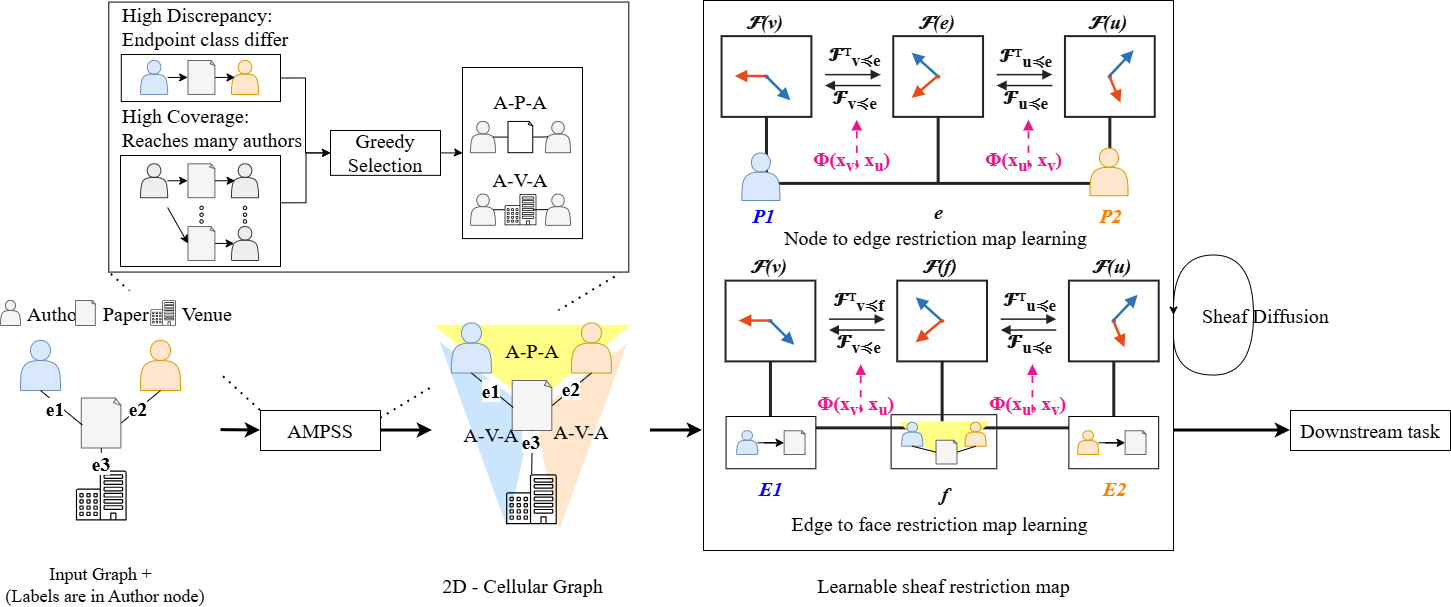
\includegraphics[width=\textwidth]{figure/h2snn_framework_overview.png}
  \caption{Overview of \method{}.  Typed graph data enter a training-only \ampss{} selection stage;
  selected schemas and weighted path instances then parameterize the node-edge-face geometry.
  Node and edge cochains diffuse in parallel before task-specific node, link, or graph prediction,
  with graph classification routed through \sheafconvpool{}.}
  \Description{A left-to-right four-stage diagram.  Data Input feeds AMPSS schema and instance
  selection, which feeds H2S-NN sheaf-Hodge geometry and parallel node and edge diffusion.  The
  output branches to node classification, link prediction, and graph classification through
  SheafConvPool.}
  \label{fig:pipeline}
\end{figure*}

\subsection{Task-Specific Input Preprocessing}

All three tasks start from the same representation.  The heterogeneous graph is flattened into one
node table and one directed edge table that retain each node's type and each edge's relation type,
and raw features are zero-padded to a common width, written \(x_v\).  What differs across tasks is
the supervision available to describe how relations behave; in every case it is derived from the
training split alone, and validation and test labels or links never enter this stage.

\paragraph{Node classification.}
A single label-propagation pass, clamped to the training labels, gives every node a soft class
distribution \(\widehat y_v\).  For each relation type we then record four endpoint-agreement
scores: between propagated class distributions, between structural summaries such as degree and
typed-path counts, between feature-derived summaries, and as normalized mutual information between
the endpoint distributions.  Stacked over all relations, these form one global vector
\(m\in\R^{4|\mathcal{R}|}\) that is appended to every node,
\begin{equation}
  x_v = x_v^{\mathrm{raw}}\concat m ,
  \label{eq:feature-augmentation}
\end{equation}
so the encoder can see which relations tend to link disagreeing endpoints instead of having to
infer it from features alone.

\paragraph{Link prediction.}
No node labels exist to propagate, so the encoder receives \(x_v\) unchanged.  Instead, \ampss{}
uses a two-channel signal recording how often a node appears as the source or the target of a
training-positive edge, and consults it only when scoring candidate link schemas.

\paragraph{Graph classification.}
The diagnostic is computed per fold rather than per node.  Within the training graphs of the
current fold, \ampss{} retains typed path schemas whose presence differs across classes, so the
schema pool reflects only patterns that separate the training labels.

\subsection{Node Stalks and Sheaf Restrictions Initialization}

This stage instantiates the first-coboundary machinery for the flattened heterogeneous graph. The
type-specific encoder produces initial node stalks, and relation-conditioned restriction maps
define how each edge compares its endpoints. This is inherited sheaf structure rather than a
separate meta-path contribution; it supplies the \(\delta_0\) operator that the later
edge-to-face construction must compose with.

\paragraph{Type-specific node states.}
Different node types need not share a feature vocabulary or input dimension.  We therefore map
each type into the common stalk space before comparing adjacent nodes:
\begin{equation}
  h_v^{(0)}
  =\operatorname{Dropout}\!\left[
    \operatorname{GELU}\!\left(
      \operatorname{LN}(W_{\phi(v)}x_v+b_{\phi(v)})+q_{\phi(v)}
    \right)
  \right]\in\R^d ,
  \label{eq:node-encoder}
\end{equation}
where \(W_t,b_t\) are type-specific parameters and \(q_t\) is a learned type embedding.  A learned
node table supplies \(h_v^{(0)}\) when raw attributes are unavailable.  We initialize the diffused
node cochain as \(x^{(0)}=h^{(0)}\), and represent each relation \(r\) by
\(z_r\in\R^{d_r}\).

\paragraph{Relation-conditioned restrictions.}
Given an oriented edge \(e=(u\xrightarrow{r}v)\), two relation-conditioned networks infer
\(F_{u\unlhd e},F_{v\unlhd e}\in\R^{d\times d}\) from
\(h_u^{(0)}\), \(h_v^{(0)}\), and \(z_r\).  Each restriction is scaled orthogonal:
\begin{equation}
  F_{v\unlhd e}=\lambda_{v,e}Q_{v,e},
  \qquad Q_{v,e}^{\transpose}Q_{v,e}=I,
  \qquad \lambda_{v,e}>0 ,
  \label{eq:conformal-map}
\end{equation}
and analogously for \(F_{u\unlhd e}\).  The orthogonal factor aligns local coordinates, while the
positive scale adjusts the strength of the incidence.  These restrictions define the first
coboundary immediately:
\begin{equation}
  (\delta_0x)_e
  =F_{v\unlhd e}x_v-F_{u\unlhd e}x_u .
  \label{eq:delta0}
\end{equation}
Thus, \(\delta_0x\) measures endpoint disagreement after relation-specific transport rather than
raw feature difference.

\paragraph{Independent edge initialization.}
Endpoint disagreement is informative, but it need not span every useful edge signal.  We initialize
the edge cochain with a separate network,
\begin{equation}
  s_e^{(0)}
  =\operatorname{MLP}_{\mathrm{init}}\!\left(
    h_u^{(0)}\concat h_v^{(0)}\concat z_r
    \concat(\delta_0h^{(0)})_e
  \right),
  \label{eq:edge-init}
\end{equation}
so \(s^{(0)}\neq\delta_0h^{(0)}\) in general.  This preserves an edge component outside
\(\operatorname{im}\delta_0\) for the subsequent lower- and upper-Hodge interactions.

\subsection{\ampss{}: Adaptive Meta-Path Schema-to-Cell Selection}
\label{sec:ampss}

\ampss{} separates economical structure search from task-driven refinement.  The first stage is a
non-differentiable, training-only construction of a candidate pool; the second stage learns soft
weights for the retained schemas and their concrete instances jointly with \method{}.

\paragraph{Stage I: candidate generation and preselection.}
The first stage constructs a small set of typed higher-order supports before the neural model is
trained.  It does so at the level of the heterogeneous schema rather than by immediately traversing
all concrete node paths.  We first form a directed type graph whose nodes are entity types and whose
directed edges are relation types, e.g., \(P\xrightarrow{\mathrm{writes}^{-1}}A\) and
\(A\xrightarrow{\mathrm{writes}}P\) in a paper--author network.  A bounded depth-first search over
this type graph enumerates valid schema candidates
\(\sigma=(t_0,r_1,t_1,\ldots,r_\ell,t_\ell)\) subject to the allowed length range and, when
required by the task, the start and end target types.  This step therefore proposes only type-valid
relational routes; it does not yet decide that any route is useful.

For each candidate schema, \ampss{} then samples concrete instances in the original graph.  Starting
from nodes of type \(t_0\), it follows the prescribed relation sequence
\((r_1,\ldots,r_\ell)\) and records paths
\(f=(v_0,e_1,v_1,\ldots,e_\ell,v_\ell)\) whose node and edge types match the schema.  Separate
budgets cap the number of candidate schemas, the number of instances expanded from one anchor node,
the number of instances retained for one schema, and the total number of materialized instances.
These caps make the construction economical while still exposing the model to the main typed
relational patterns present in the graph.

The preselection score is designed to keep schemas that are both informative and usable as
face-like supports.  For node classification, training labels are propagated for a fixed number of
steps to obtain soft endpoint distributions \(\widehat y_v\).  A concrete path receives a large
discrepancy when its two endpoints carry different training-derived class evidence, and a schema
receives the average discrepancy of its sampled instances:
\begin{equation}
  d(f)=\norm{\widehat y_{v_0}-\widehat y_{v_\ell}}_2^2,
  \qquad
  D(\sigma)=\frac{1}{|\mathcal{I}_{\sigma}|}
  \sum_{f\in\mathcal{I}_{\sigma}}d(f).
  \label{eq:discrepancy}
\end{equation}
Intuitively, this favors schemas whose endpoints expose nontrivial class contrast under the
training signal, which can create useful edge-level disagreement for the subsequent Hodge diffusion.
For link prediction, the same idea is implemented with two propagated endpoint-role channels that
mark source and target positions using training-positive edges only.  Neither validation nor test
labels or links contribute to these statistics.

For graph classification, endpoint discrepancy is not the relevant signal.  Let
\(n_{\sigma,c}^{\mathrm{pres}}\) be the number of training graphs of class \(c\) in which schema
\(\sigma\) occurs, \(N_c\) the number of training graphs in that class, and \(n_\sigma\) the total
number of its materialized instances.  The presence score is
\begin{equation}
  P_G(\sigma)
  =\operatorname{Var}_{c}\!\left(
    \frac{n_{\sigma,c}^{\mathrm{pres}}}{\max(N_c,1)}
  \right)+10^{-3}\log(1+n_\sigma).
  \label{eq:graph-presence-score}
\end{equation}
This favors schemas whose presence differs across training classes, with frequency used only as a
small tie breaker.

For node and link tasks, \ampss{} greedily builds the selected pool one schema at a time.  The
score combines four quantities.  The discrepancy \(D(\sigma)\) measures task relevance.  The
endpoint coverage \(C(\sigma)\) measures how many target-type endpoints are reached by the sampled
instances, so a schema that appears only in a tiny corner of the graph is not selected merely
because it has a high local score.  The type diversity \(V(\sigma)\) rewards schemas that pass
through multiple semantic types rather than repeatedly using the same type pattern.  Finally,
\(J(\sigma,\sigma')\) measures endpoint-set overlap with an already selected schema
\(\sigma'\), discouraging several selected schemas from describing nearly the same region of the
graph.  Given the current pool \(S\), the greedy score is
\begin{equation}
  q(\sigma\mid S)=
  \frac{D(\sigma)^{a_d}C(\sigma)^{a_c}V(\sigma)^{a_v}}
       {1+\max_{\sigma'\in S}J(\sigma,\sigma')} ,
  \label{eq:topology-score}
\end{equation}
The numerator prefers schemas that are informative, sufficiently covered, and semantically varied;
the denominator lowers the priority of schemas that are redundant with the pool already chosen.
Graph tasks use the class-presence score \(P_G(\sigma)\) instead of Equation~\ref{eq:topology-score}.
After this greedy pass, the selected schemas are materialized as ordered path supports, together
with the closure pairs used by the node-side correction.  This entire stage fixes the candidate
support and is intentionally non-differentiable; the next stage decides how strongly the retained
schemas and their individual instances should participate in the learned operator.

\paragraph{Stage II: differentiable schema and instance refinement.}
Preselection decides what can be considered; it does not force every retained structure to
contribute equally.  We learn one gate per schema and a state-dependent gate for every path
instance:
\begin{equation}
  \begin{aligned}
  \alpha_\sigma&=\operatorname{sigmoid}(\theta_\sigma),\\
  \beta_f&=\operatorname{sigmoid}\!\left(
    g_\beta(h_{v_0}^{(0)}\concat h_{v_\ell}^{(0)}\concat e_\sigma)
  \right),\\
  w_f&=\alpha_{\sigma(f)}\beta_f .
  \end{aligned}
  \label{eq:gates}
\end{equation}
Here \(e_\sigma\) is a learned schema embedding.  Schema logits are warm-started from standardized
preselection scores, while \(\beta_f\) lets two instances of the same schema have different
effects.  During training, partial-schema propagation retains each schema with probability
\(p_{\mathrm{keep}}\) and rescales a retained gate by \(1/p_{\mathrm{keep}}\), following the
stabilization idea of partial message propagation \cite{li2023pmmm}.

The discovery loss applies complementary pressures rather than a single hard selection rule:
\begin{equation}
  \begin{aligned}
  \cL_{\mathrm{disc}}={}&
  \lambda_s\cL_{\mathrm{sparse\text{-}schema}}
  +\lambda_i\cL_{\mathrm{sparse\text{-}instance}}
  +\lambda_r\cL_{\mathrm{redundancy}}\\
  &+\lambda_v\cL_{\mathrm{coverage}}
  +\lambda_{\mathrm{cost}}\cL_{\mathrm{cost}}
  +\lambda_H\cL_{\mathrm{entropy}} .
  \end{aligned}
  \label{eq:discovery-loss}
\end{equation}
Schema and instance terms discourage diffuse activation; redundancy penalizes similar active
coverage profiles; the negative coverage reward discourages a trivial empty pool; cost suppresses
long, frequently instantiated schemas; and entropy minimization sharpens schema decisions.  These
terms refine only the preselected pool and do not make candidate generation differentiable.

\begin{algorithm}[t]
  \caption{\ampss{} candidate preselection and differentiable refinement}
  \label{alg:ampss}
  \begin{algorithmic}[1]
    \REQUIRE Typed relation graph, training split, schema and instance budgets
    \STATE \textbf{Stage I: Candidate generation and training-only preselection}
    \STATE Enumerate bounded typed schemas and sample concrete instances
    \STATE Compute node/link discrepancy scores or graph presence scores
    \STATE Greedily retain a compact pool \(\Sigma\) and materialize its path supports
    \STATE Initialize \(\theta_\sigma\) from standardized preselection scores
    \FOR{each training epoch}
      \STATE \textbf{Stage II: Differentiable schema and instance refinement}
      \STATE Use uniform face weights during warm-up
      \STATE Compute \(\alpha_\sigma\), \(\beta_f\), and \(w_f=\alpha_{\sigma(f)}\beta_f\)
      \STATE Apply partial-schema propagation with keep probability \(p_{\mathrm{keep}}\)
      \STATE Run matrix-free sheaf-Hodge diffusion and the task readout
      \STATE Optimize Equation~\ref{eq:loss}
    \ENDFOR
  \end{algorithmic}
\end{algorithm}

\subsection{2D-cellular Sheaf-Hodge Geometry Construction}

A cellular complex represents a structure using cells of different dimensions. General graphs are 1-D cellular complexes where Nodes are $0$-cells, edges are $1$-cells. Unlike another sheaf diffusion network that works on 1-D cellular complexes graph \cite{bodnar2022neural,braithwaite2024heterogeneous,ribeiro2026cooperative,barbero2022sheaf}, however, for our \method{} we construct graphs as 2-D cellular complexes by adding faces produces a two-dimensional complex. We
write $\sigma\unlhd\tau$ when a lower-dimensional cell $\sigma$ is incident to a
higher-dimensional cell $\tau$. A cellular sheaf $\cF$ equips each cell $\sigma$ with a local
vector space, or \emph{stalk}, $\cF(\sigma)$, and assigns a linear restriction map
$F_{\sigma\unlhd\tau}:\cF(\sigma)\rightarrow\cF(\tau)$ to every incident pair. These maps transport
information from different cells into common spaces and must compose consistently along incidence
chains.

On a graph $G=(V,E)$, the relevant stalks live on nodes and edges. For each incident pair
$v\unlhd e$, the restriction map $F_{v\unlhd e}:\cF(v)\rightarrow\cF(e)$ transports the node
representation into the shared edge space. Node and edge assignments form the cochain spaces
\begin{equation}
  C^0(G,\cF)=\bigoplus_{v\in V}\cF(v),
  \qquad
  C^1(G,\cF)=\bigoplus_{e\in E}\cF(e).
\end{equation}

Given an oriented edge $e=(u\rightarrow v)$, the first coboundary operator
$\delta_0:C^0(G,\cF)\rightarrow C^1(G,\cF)$ measures disagreement between the transported endpoint
representations:
\begin{equation}
  (\delta_0x)_e
  =
  F_{v\unlhd e}x_v-F_{u\unlhd e}x_u.
  \label{eq:background-delta0}
\end{equation}
The corresponding sheaf Laplacian is
$L_0=\delta_0^{\transpose}\delta_0$, with energy
$x^{\transpose}L_0x=\lVert\delta_0x\rVert_2^2$. When all stalks are one-dimensional and all
restriction maps are identities, $L_0$ reduces to the ordinary graph Laplacian.

\subsection{Path-Supported Edge-Face Geometry}
\label{sec:face-geometry}

Consider a selected \(P\!-\!A\!-\!P\) instance
\(f=(v_0,e_1,v_1,e_2,v_2)\).  The model retains the ordered path edges
\(\partial_{\mathrm{path}}f=(e_1,e_2)\) as the path part of the boundary: it does not replace the instance by
a shortcut edge between its endpoint papers.  For a general instance
\(f=(v_0,e_1,v_1,\ldots,e_\ell,v_\ell)\), an edge token combines its endpoint states and relation,
\begin{equation}
  \begin{aligned}
  g_i&=\operatorname{MLP}_g\!\left(
    h_{v_{i-1}}^{(0)}\concat h_{v_i}^{(0)}\concat z_{\psi(e_i)}
  \right),\\
  (o_1,\ldots,o_\ell)&=\operatorname{LSTM}(g_1,\ldots,g_\ell).
  \end{aligned}
\end{equation}
The ordered encoder distinguishes positions along the path.  Attention then pools the sequence into
a single summary, which produces one free map per instance:
\begin{equation}
  \pi_{fi}
  =\operatorname{softmax}_{i}\!\left(
    \frac{o_i^{\transpose}a}{\sqrt{d_h}}
  \right),
  \qquad
  A_f
  =\operatorname{reshape}\!\Big(W_F\textstyle\sum_i\pi_{fi}o_i+b_F,\,d,d\Big).
  \label{eq:face-map}
\end{equation}
Attention shapes \(A_f\); it deliberately does not rescale individual edges' maps, because a
non-uniform per-edge factor would destroy the boundary cancellation established below.

The per-edge maps are then \emph{not} emitted independently.  A cellular sheaf is a functor on the
face poset, so an edge-to-face map must compose with the node-to-edge maps beneath it; emitting both
from separate networks breaks that functoriality, and with it the cochain property.  We therefore
carry a transport to the base vertex \(v_0\) along the boundary:
\begin{equation}
  \begin{aligned}
  T_{v_0}&=A_f,
  \qquad
  T_{v_i}=T_{v_{i-1}}F_{u\unlhd e_i}^{-1}F_{v\unlhd e_i},\\
  F_{e_i\unlhd f}&=T_{v_{i-1}}F_{u\unlhd e_i}^{-1},
  \end{aligned}
  \label{eq:transport}
\end{equation}
where \(u=v_{i-1}\) and \(v=v_i\) are the endpoints of \(e_i\).  The inverse is available in closed
form: by Eq.~\eqref{eq:conformal-map} each map is a positive scale times an orthogonal factor, so
\(F^{-1}=F^{\transpose}/\lambda^2\), and no linear solve is required.  Each map
\(F_{e_i\unlhd f}:\cF(e_i)\rightarrow\cF(f)\) still transports the \(i\)-th edge state into the
shared face stalk, and still varies per instance and per relation; what changes is that a single
\(d\times d\) matrix per instance is learned freely rather than \(\ell\) of them.

Let \(\eta(e,f)\in\{-1,+1\}\) be the stored incidence orientation.  The face gate enters the
weighted second coboundary:
\begin{equation}
  (\delta_{1,w}s)_f
  =\sqrt{w_f}\sum_{e\in\partial f}
    \eta(e,f)F_{e\unlhd f}s_e .
  \label{eq:delta1}
\end{equation}
Writing
\(B_fs=\sum_{e\in\partial f}\eta(e,f)F_{e\unlhd f}s_e\), its upper-Hodge
contribution is therefore
\begin{equation}
  \delta_{1,w}^{\transpose}\delta_{1,w}
  =\sum_{\sigma\in\Sigma}\sum_{f\in\mathcal{I}_{\sigma}}
    w_f B_f^{\transpose}B_f .
  \label{eq:weighted-up}
\end{equation}
The square root is important: it makes each face contribute linearly in \(w_f\), not quadratically.

An open path is not the boundary of a \(2\)-cell: a cell is attached along a cycle.  Each instance
therefore also carries a synthetic closure \(1\)-cell \(e_{\mathrm{cl}}=(v_\ell\rightarrow v_0)\),
oriented along the cycle, which completes \(\partial f=(e_1,\ldots,e_\ell,e_{\mathrm{cl}})\).  It is a
stateful edge with its own stalk, and its restriction maps are \emph{defined} rather than learned:
\begin{equation}
  F_{v_0\unlhd e_{\mathrm{cl}}}=I,
  \qquad
  F_{v_\ell\unlhd e_{\mathrm{cl}}}=T_{v_0}^{-1}T_{v_\ell},
  \qquad
  F_{e_{\mathrm{cl}}\unlhd f}=A_f .
  \label{eq:closure-maps}
\end{equation}
The middle map reduces to \(\prod_i F_{u\unlhd e_i}^{-1}F_{v\unlhd e_i}\), the holonomy of the path
itself: it is independent of \(A_f\) and adds no parameters.  The closure cell is thus a bookkeeping
device that makes ``traverse this path and return'' well posed, not an asserted relation between the
endpoints.  Figure~\ref{fig:sheaf-hodge-operator} makes this boundary explicit.

\begin{proposition}[Exact cochain condition]
\label{prop:chain}
For every instance whose node sequence is a simple path, the maps of
Eqs.~\eqref{eq:transport}--\eqref{eq:closure-maps} satisfy
\(\delta_{1,w}\delta_0=0\) identically, for every node cochain and every value of the learned
parameters, with no assumption that the sheaf has trivial holonomy.
\end{proposition}

\begin{proof}
By construction \(F_{e_i\unlhd f}F_{u\unlhd e_i}=T_{v_{i-1}}\) and
\(F_{e_i\unlhd f}F_{v\unlhd e_i}=T_{v_i}\), so the \(i\)-th boundary term of \(\delta_{1,w}\delta_0x\)
equals \(T_{v_i}x_{v_i}-T_{v_{i-1}}x_{v_{i-1}}\), and summing over the path telescopes to
\(T_{v_\ell}x_{v_\ell}-T_{v_0}x_{v_0}\).  Eq.~\eqref{eq:closure-maps} gives
\(F_{e_{\mathrm{cl}}\unlhd f}F_{v_0\unlhd e_{\mathrm{cl}}}=T_{v_0}\) and
\(F_{e_{\mathrm{cl}}\unlhd f}F_{v_\ell\unlhd e_{\mathrm{cl}}}=T_{v_\ell}\), so the closure term
contributes \(T_{v_0}x_{v_0}-T_{v_\ell}x_{v_\ell}\) and the total vanishes.  Simplicity is required
because the transport assigns one map per node position; a revisited node — including a coincident
endpoint pair — would be assigned two values.
\end{proof}

\noindent Empirically the residual \(\norm{\delta_{1,w}\delta_0h^{(0)}}/\norm{\delta_0h^{(0)}}\) is
at the level of single-precision roundoff (\(\sim\!10^{-7}\)) on all evaluated datasets, for both
manual and \ampss{} schema sets.

\begin{figure}[t]
  \centering
  \fbox{\rule{0pt}{4.2cm}\rule{0.94\columnwidth}{0pt}}
  %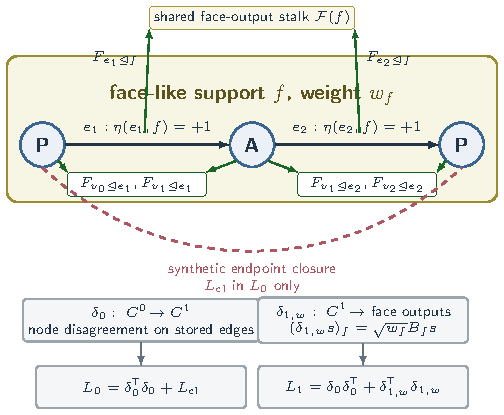
\includegraphics[width=\columnwidth]{figure/h2snn_sheaf_hodge_operator.pdf}
  \caption{AMPSS-selected path instances define a sheaf-Hodge operator. Currently in construction.}
  \label{fig:sheaf-hodge-operator}
\end{figure}

\subsection{Matrix-Free Sheaf-Hodge Diffusion}
\label{sec:closure}

The two coboundaries induce one node operator and one edge operator:
\begin{align}
  L_0x
  &=\delta_0^{\transpose}\delta_0x,
  \label{eq:l0}\\
  L_1s
  &=\underbrace{\delta_0\delta_0^{\transpose}s}_{\text{lower edge term}}
    +\underbrace{\delta_{1,w}^{\transpose}\delta_{1,w}s}_{\text{upper edge term}} .
  \label{eq:l1}
\end{align}
The lower edge term compares edge signals through their incident nodes; the upper term couples the
edges of a boundary cycle through their shared face.  Because the closure \(1\)-cell of
Section~\ref{sec:face-geometry} is an ordinary member of the edge set, it enters \(\delta_0\) — and hence
\(L_0\) and the lower edge term — exactly like a data edge; no separate node-side correction is
applied.  Its restriction maps are the path holonomy of Eq.~\eqref{eq:transport}, so it introduces
no parameters of its own, and a scale \(\gamma>0\) on them is absorbed by the compensating factor in
\(F_{e_{\mathrm{cl}}\lhd f}\), leaving Proposition~\ref{prop:chain} unaffected while tuning how
strongly the boundary cycle closes at the node level.

Starting from \(x^{(0)}=h^{(0)}\) and the independent \(s^{(0)}\), \(K\) explicit Euler steps give
\begin{equation}
  \begin{aligned}
  x^{(k+1)}&=x^{(k)}-\eta_0L_0x^{(k)},\\
  s^{(k+1)}&=s^{(k)}-\eta_1L_1s^{(k)},
  \qquad k=0,\ldots,K-1 .
  \end{aligned}
  \label{eq:diffusion}
\end{equation}
The positive step sizes may be learned.  Node and edge cochains evolve in parallel under geometry
inferred from the same initial node states; there is no cross-rank recurrence between Euler steps.
Layer normalization yields the terminal states \(x^\star\) and \(s^\star\).

Execution is matrix-free: the model applies restrictions in batches and aggregates incident
contributions, without materializing global \(Nd\times Nd\) or \(Md\times Md\) matrices.  Three
implementation boundaries remain consequential.  First, \(\delta_{1,w}\) spans the complete boundary
cycle: the \(\ell\) path edges together with the closure \(1\)-cell.  Second, signed incidences are
supported, and the uniform \(+1\) used here is the correct boundary map precisely because
enumeration traverses every edge along its stored direction and stores the closure cell oriented
along the cycle; the pipeline asserts this rather than assuming it, so a future change to reverse
traversal fails loudly instead of silently invalidating the signs.  Third, because faces must be
simple paths for the transport of Eq.~\eqref{eq:transport} to be well defined, instances that revisit
a node — including those whose endpoints coincide — are excluded during enumeration.  On the
manual meta-path templates this removes a negligible fraction of instances, since the search
backfills its per-anchor budget with simple paths.  Unlike earlier path-supported sheaf
constructions, \(\delta_{1,w}\delta_0=0\) is not encouraged by a penalty but holds identically
(Proposition~\ref{prop:chain}).

\subsection{Downstream Readouts}
\label{sec:readouts}

\paragraph{Node classification.}
Let
\(\bar s_v^\star=|E(v)|^{-1}\sum_{e\ni v}s_e^\star\), with a zero vector for an isolated node.
The target-node classifier retains the terminal node state, the pre-diffusion state, and the local
edge summary:
\begin{equation}
  \widehat y_v
  =\operatorname{MLP}_{\mathrm{node}}\!\left(
    x_v^\star\concat h_v^{(0)}\concat\bar s_v^\star
  \right).
  \label{eq:node-readout}
\end{equation}
The third view gives the supervised node head direct access to information transformed by the
upper edge operator.

\paragraph{Link prediction.}
Candidate endpoints are decoded from their final node states using a dot product, a
relation-conditioned DistMult decoder, or a concatenation MLP.  The current link head does not
directly consume \(s^\star\); consequently, its task loss reaches the upper-edge pathway only
through shared training terms, not through an edge-state link decoder.

\paragraph{Graph classification.}
A graph head must be invariant under node and edge permutations and orthogonal stalk gauges.
\sheafconvpool{} meets these requirements while retaining both terminal and initial node views and
the learned edge cochain.  It is a single-level terminal readout.

\subsection{\sheafconvpool{}}

For each node \(v\), \sheafconvpool{} stacks three aligned views,
\begin{equation}
  Z_v^{(0)}
  =\begin{bmatrix}x_v^\star&h_v^{(0)}&\bar s_v^\star\end{bmatrix}
  \in\R^{d\times3}.
\end{equation}
For each stored edge \(e\), it similarly forms
\begin{equation}
  Z_e^{(1)}
  =\begin{bmatrix}
    (\delta_0x^\star)_e&(\delta_0h^{(0)})_e&s_e^\star
  \end{bmatrix}
  \in\R^{d\times3}.
\end{equation}
The corresponding \(3\times3\) Gram descriptors are
\(G_i^{(r)}=(Z_i^{(r)})^{\transpose}Z_i^{(r)}\), for rank \(r\in\{0,1\}\).
Under an orthogonal local gauge \(Z_i^{(r)}\mapsto Q_iZ_i^{(r)}\),
\(G_i^{(r)}\) is unchanged.  The readout therefore learns only from coordinate-independent
inner products among its three views.

Separate node and edge networks project the flattened descriptors,
\(u_i^{(r)}=\rho_r(\operatorname{vec}G_i^{(r)})\in\R^{d_p}\), and score them with invariant
attention.  Within each graph and rank,
\begin{equation}
  a_i^{(r)}
  =\frac{\exp(g_r(u_i^{(r)}))}
         {\sum_{j\in\mathcal{C}_r}\exp(g_r(u_j^{(r)}))},
  \qquad
  \mu_r=\sum_{i\in\mathcal{C}_r}a_i^{(r)}u_i^{(r)},
\end{equation}
where \(\mathcal{C}_0\) and \(\mathcal{C}_1\) are the graph's nodes and edges.  A mean alone cannot
record whether informative descriptors are concentrated or dispersed, so the readout also computes
\begin{equation}
  \Sigma_r
  =\sum_{i\in\mathcal{C}_r}a_i^{(r)}
    (u_i^{(r)}-\mu_r)(u_i^{(r)}-\mu_r)^{\transpose}.
\end{equation}
The graph representation concatenates
\(\mu_0\), the upper triangle of \(\Sigma_0\), \(\mu_1\), and the upper triangle of
\(\Sigma_1\); an MLP maps this vector to graph logits.  Softmax normalization and moment summation
make the construction permutation invariant, while the Gram descriptors make it invariant under
the model's orthogonal stalk gauges.

\begin{figure}[t]
  \centering
  \fbox{\rule{0pt}{4.2cm}\rule{0.94\columnwidth}{0pt}}
  %\includegraphics[width=\columnwidth]{figure/sheafconvpool_architecture.pdf}
  \caption{\sheafconvpool{} graph readout.  Node and edge view stacks become orthogonal-gauge
  invariant through \(Z^{\transpose}Z\).  Separate projections and invariant attention produce
  weighted means and covariances; their node/edge summaries are concatenated for graph
  classification. The actual picture is currently in construction.}
  \Description{Two parallel node and edge branches.  Each starts with three stalk-valued views,
  forms a Gram descriptor, applies a learned projection and invariant attention, and computes a
  weighted mean and covariance.  Upper-triangular covariance vectors join the means, and the two
  branches concatenate before an MLP outputs graph logits.}
  \label{fig:sheafconvpool}
\end{figure}

\subsection{Training Objective}

The geometry carries no auxiliary loss.  The task term is cross-entropy for single-label node and
graph classification, binary cross-entropy for multi-label classification and link prediction, with
the appropriate training mask or sampled training pairs, and the only additional term is the
\ampss{} schema-selection objective:
\begin{equation}
  \cL
  =\cL_{\mathrm{task}}
   +\rho(t)\cL_{\mathrm{disc}} .
  \label{eq:loss}
\end{equation}
During discovery warm-up, gates are bypassed by uniform face weights and \(\rho(t)=0\).  After
warm-up, the schema and instance gates activate; \(\rho(t)\) is either applied at full strength or
annealed linearly to one over a configured interval.  This schedule lets task gradients establish a
useful path geometry before sparsity, redundancy, and cost pressures dominate.  For manual schema
sets \(\cL_{\mathrm{disc}}\) is absent and the objective reduces to the task loss alone.

That the geometric terms are absent is a consequence of the construction, not an omission.  A chain
penalty is unnecessary because Proposition~\ref{prop:chain} makes \(\delta_{1,w}\delta_0\) vanish
identically; on an open path such a penalty is in any case unsatisfiable except by degenerate face
maps, since the two endpoint blocks of \(\delta_{1,w}\delta_0\) each appear in a single term while the
node-to-edge maps are invertible.  A consistency penalty \(\norm{s^\star-\delta_0x^\star}^2\) is
counterproductive: \(x\) evolves under \(L_0\) alone and the edge channel never feeds back into it, so
driving \(s^\star\) to \(\delta_0x^\star\) would make the edge cochain a deterministic image of the
node cochain and the faces would contribute nothing.  A face-level Dirichlet penalty
\(\norm{\delta_{1,w}s^\star}^2\) is counterproductive for the same reason at one rank higher: with the
cochain condition exact, \(\delta_{1,w}s^\star\) is precisely the curl component of the edge cochain
and the only part the upper Hodge term \(\delta_{1,w}^{\transpose}\delta_{1,w}\) acts on, so shrinking
it drives the face branch inert.  The edge cochain is therefore left free at both ranks.


\section{Experiments}
\label{sec:experiments}

We evaluated \method{} with \ampss{} on a range of heterogeneous graph tasks, including node classification, link prediction, and graph classification. On the graph classification task, we also evaluated the single-level \sheafconvpool{} readout.

In general, the model selection was performed using hyperparameter sweeps. The full per-dataset hyperparameters are listed in Appendix~\ref{app:hyperparameters}. The code is available at \url{placeholder_for_code_repository.com}.

In Tables~\ref{tab:node-cls}, \ref{tab:graph-cls}, and \ref{tab:link-pred}, we group the baselines introduced in each subsection’s \emph{Baselines} paragraph into four categories: Hom./hom., Het./hom., Hom./het., and Het./het. The first term indicates whether the model assumes a homogeneous or heterogeneous graph, while the second indicates whether it is designed for homophilic or heterophilic settings. \method{} is reported separately under Ours. Since HetSheaf does not provide a public implementation, we report the results published in its original paper, which follows the same experimental settings as ours. To ensure a fair comparison, we conducted the experiments with 5 different random seeds and reported the average performance with standard deviation.


\subsection{Node Classification}
\label{sec:setup-node}


\paragraph{Datasets}
On the node classification task, we used three benchmark heterogeneous graph datasets: DBLP \cite{lv2021hgb} and IMDB \cite{lv2021hgb}, and ACM \cite{wang2019han}. The statistics of these datasets are summarized in Table~\ref{tab:node-datasets}.

\begin{table}[H]
  \centering
  \caption{Node-classification datasets and their semantic meta-paths. The N column indicates nodes, E indicates the number of edges, and C indicates classes.}
  \label{tab:node-datasets}
  \scriptsize
  \resizebox{\columnwidth}{!}{%
  \begin{tabular}{lrrrrrll}
    \toprule
    \textbf{Dataset} & \textbf{\#N} & \textbf{\#N types} & \textbf{\#E} &
    \textbf{\#E types} & \textbf{Classes} & \textbf{Target} & \textbf{Meta-paths} \\
    \midrule
    DBLP & 26{,}128 & 4 & 239{,}566 & 6 & 4 & author & APA, APCPA, APTPA \\
    IMDB & 21{,}420 & 4 & 86{,}642 & 6 & 5 & movie & MAM, MDM \\
    ACM & 10{,}942 & 4 & 547{,}806 & 7 & 3 & paper & PAP, PSP \\
    \bottomrule
  \end{tabular}%
  }
\end{table}


\paragraph{Baselines.} We compared \method{} against four groups of baselines: (i) homogeneous homophilic models, including GCN
\cite{kipf2017gcn}, GAT \cite{velickovic2018gat}, and ChebNetII \cite{he2022chebnetii}; (ii) homogeneous heterophilic models, including NSD
\cite{bodnar2022neural} and CSNN \cite{ribeiro2026cooperative}; (iii)
heterogeneous homophilic models, including HAN \cite{wang2019han}, SeHGNN \cite{yang2023sehgnn},
HiNormer \cite{mao2023hinormer}, and PSHGCN \cite{he2024spectral}; and heterogeneous heterophilic models, including HDHGR \cite{guo2023homophily}, Hetero$^2$Net \cite{li2025hetero2net}, H2SGNN
\cite{lu2026addressing}, HetSheaf \cite{braithwaite2024heterogeneous}, and LatGRL
\cite{shen2025heterophily}.


\paragraph{Evaluation Settings.} For the node classification tasks experimental settings, we followed the HGB benchmark \cite{lv2021hgb} by using the training/validation/test splits in a ratio of 20\%/20\%/60\% on transductive learning. We used Macro-F1 and Micro-F1 as the evaluation metrics. For our \method{}, we conducted the experiment by including \ampss{}. 

\paragraph{Results.}
From the results in Table~\ref{tab:node-cls}, \method{} achieved the best performance on all three benchmark datasets in node classification tasks. \method{} outperforms every method that addresses heterogeneity without heterophily (Het./hom.) or heterophily on homogeneous graphs (Hom./het.), consistent with treating type-aware restriction and heterophily-robust comparison as complementary rather than substitutable. Against the strongest heterogeneous heterophilic (Het./het.) baselines, which already combine both properties, the remaining margin is consistent but smaller, which we attribute to \method{} additionally retaining concrete meta-path instances as operator-level structure rather than only adjusting node-level message passing.

\begin{table*}[t]
  \centering
  \caption{Performance on node classification benchmarks reporting in Macro-F1 and Micro-F1. Best values are bold.}
  \label{tab:node-cls}
  \scriptsize
  \resizebox{0.8\textwidth}{!}{%
  \begin{tabular}{llcccccc}
    \toprule
    & &
    \multicolumn{2}{c}{DBLP (59.76)} &
    \multicolumn{2}{c}{ACM (72.39)} &
    \multicolumn{2}{c}{IMDB (50.04)} \\
    \cmidrule(lr){3-4}
    \cmidrule(lr){5-6}
    \cmidrule(lr){7-8}
    \textbf{Group} & \textbf{Model}
    & Macro & Micro
    & Macro & Micro
    & Macro & Micro \\
    \midrule

    \multirow{3}{*}{Hom./hom.}
    & GCN
    & $90.77 \pm 0.76$
    & $90.28 \pm 0.20$
    & $91.63 \pm 0.44$
    & $91.38 \pm 0.39$
    & $62.33 \pm 0.58$
    & $67.69 \pm 0.59$ \\

    & GAT
    & $94.39 \pm 1.03$
    & $92.52 \pm 0.27$
    & $92.07 \pm 0.57$
    & $90.71 \pm 0.21$
    & $62.13 \pm 0.26$
    & $68.09 \pm 0.48$ \\
    
    & ChebNetII
    & $92.89 \pm 1.07$
    & $92.67 \pm 0.50$
    & $91.70 \pm 0.27$
    & $91.59 \pm 0.27$
    & $62.97 \pm 0.66$
    & $68.47 \pm 0.55$ \\

    \midrule

    \multirow{2}{*}{Het./hom.}
    & NSD
    & $92.96 \pm 0.21$
    & $93.42 \pm 0.37$
    & $92.33 \pm 0.78$
    & $92.05 \pm 0.69$
    & $61.61 \pm 0.26$
    & $65.23 \pm 0.51$ \\


    & CSNN
    & $93.73 \pm 0.95$
    & $92.12 \pm 0.19$
    & $93.13 \pm 0.94$
    & $92.81 \pm 0.83$
    & $62.92 \pm 0.34$
    & $62.59 \pm 0.22$ \\


    \midrule

    \multirow{4}{*}{Hom./het.}
    & HAN
    & $91.78 \pm 0.92$
    & $92.24 \pm 0.86$
    & $90.88 \pm 0.67$
    & $91.61 \pm 1.07$
    & $61.95 \pm 0.36$
    & $67.76 \pm 0.51$ \\

    & SeHGNN
    & $95.52 \pm 0.98$
    & $95.48 \pm 0.78$
    & $94.38 \pm 1.00$
    & $94.04 \pm 0.73$
    & $72.01 \pm 0.65$
    & $72.59 \pm 0.18$ \\

    & HiNormer
    & $94.06 \pm 0.40$
    & $94.14 \pm 0.46$
    & $91.87 \pm 0.26$
    & $89.64 \pm 0.39$
    & $64.13 \pm 0.19$
    & $67.53 \pm 0.32$ \\

    & PSHGCN
    & $95.58 \pm 0.80$
    & $95.70 \pm 0.54$
    & $93.66 \pm 0.53$
    & $94.70 \pm 0.39$
    & $71.82 \pm 0.34$
    & $74.34 \pm 0.84$ \\
    \midrule

    \multirow{5}{*}{Het./het.}
    & HDHGR
    & $95.35 \pm 0.81$
    & $95.00 \pm 0.77$
    & $93.99 \pm 0.35$
    & $94.13 \pm 0.87$
    & $59.41 \pm 0.22$
    & $59.63 \pm 0.35$ \\

    & Hetero2Net
    & $93.54 \pm 1.11$
    & $93.54 \pm 0.79$
    & $94.05 \pm 0.71$
    & $92.87 \pm 0.82$
    & $65.34 \pm 0.68$
    & $70.63 \pm 0.69$ \\

    & H2SGNN
    & $95.82 \pm 0.41$
    & $95.11 \pm 0.22$
    & $94.90 \pm 0.49$
    & $94.08 \pm 0.44$
    & $74.23 \pm 0.31$
    & $75.29 \pm 0.86$ \\

    & HetSheaf
    & $93.87 \pm 0.00$
    & $93.77 \pm 0.00$
    & $95.09 \pm 0.00$
    & $94.94 \pm 0.00$
    & $64.65 \pm 0.00$
    & $67.18 \pm 0.00$ \\

    & LatGRL
    & $94.32 \pm 0.44$
    & $94.51 \pm 0.42$
    & $93.47 \pm 0.71$
    & $92.29 \pm 0.43$
    & $58.27 \pm 0.46$
    & $58.81 \pm 0.65$ \\
    \midrule

    Ours
    & \textbf{\method{}}
    & $\mathbf{96.01 \pm 0.58}$
    & $\mathbf{96.31 \pm 0.40}$
    & $\mathbf{95.91 \pm 1.15}$
    & $\mathbf{95.72 \pm 0.68}$
    & $\mathbf{75.05 \pm 0.22}$
    & $\mathbf{76.68 \pm 0.19}$ \\
    \bottomrule
  \end{tabular}%
  }
\end{table*}



\subsection{Graph classification}
\label{sec:setup-graph}
\paragraph{Datasets.}
On the graph classification task, we used four benchmark heterogeneous graph datasets from TUDataset \cite{morris2020tudataset}: biological graphs, including PROTEINS and ENZYMES, and chemical compound graphs, including MUTAG and NCI1. To make those graphs heterogeneous, we treated the node and edge labels supplied by TUDataset as different node and edge types. Table~\ref{tab:graph-datasets} gives the statistics of the four TUDataset graph-classification benchmarks.

\begin{table}[H]
  \centering
  \caption{Graph-classification dataset statistics. The N column indicates nodes, E indicates the number of edges, and C indicates classes.}
  \label{tab:graph-datasets}
  \small
  \resizebox{\columnwidth}{!}{%
  \begin{tabular}{lrrrrl}
    \toprule
    \textbf{Dataset} & \textbf{Graphs} & \textbf{\#N types} & \textbf{\#E} &
    \textbf{\#E types} & \textbf{Target} \\
    \midrule
    MUTAG & 188 & 7 & 7{,}442 & 4 & mutagenicity \\
    PROTEINS & 1{,}113 & 3 & 162{,}088 & 1 & enzyme/non-enzyme \\
    ENZYMES & 600 & 3 & 19{,}580 & 1 & enzyme class \\
    NCI1 & 4{,}110 & 37 & 49{,}205 & 1 & anti-cancer activity \\
    \bottomrule
  \end{tabular}%
  }
\end{table}



\paragraph{Baselines.} We compared \method{} against four groups of baselines: (i) homogeneous homophilic models, including GCN \cite{kipf2017gcn} and GAT \cite{velickovic2018gat}; (ii) homogeneous heterophilic models, including NSD \cite{bodnar2022neural} and CSNN \cite{ribeiro2026cooperative}; (iii) heterogeneous homophilic models, including HAN \cite{wang2019han} and PSHGCN \cite{he2024spectral}; and (iv) heterogeneous heterophilic models, including HDHGR \cite{guo2023homophily}, Hetero$^2$Net \cite{li2025hetero2net}, H2SGNN \cite{lu2026addressing}, HetSheaf \cite{braithwaite2024heterogeneous}, and LatGRL \cite{shen2025heterophily}.

\paragraph{Evaluation Settings.} Following the graph classification research \cite{zhang2018end, amouzad2024graphunet}, we used 10-fold cross-validation and reported the best evaluation score obtained during training. We used Macro-F1 and Micro-F1 as the evaluation metrics. For our \method{}, we conducted the experiment by including \ampss{} and \sheafconvpool{}. To ensure a fair comparison, we conducted the experiments with 5 different random seeds, each with 100 epochs for early stopping, and reported the average performance with standard deviation. For the ENZYMES dataset, we used a one-vs-rest (OVR) strategy.

\paragraph{Results.}

From the results in Table~\ref{tab:graph-cls}, \method{} achieved the best performance on all four benchmark datasets in graph classification tasks, tying the MUTAG ceiling and leading PROTEINS, ENZYMES, and NCI1 outright over every compared heterogeneous heterophilic baseline. The margin is largest on PROTEINS ($+3.88$ Macro-F1 over the closest baseline, HetSheaf), which suggests that treating the typed node and edge labels as heterogeneous structure, rather than as plain homogeneous graphs with categorical attributes, remains useful even outside the citation- and social-network domains where heterogeneity is usually studied.


\begin{table*}[t]
  \centering
  \caption{Performance on graph classification benchmarks reporting in Macro-F1 and Micro-F1. Best values are bold.}
  \label{tab:graph-cls}
  \scriptsize
  \resizebox{0.8\textwidth}{!}{%
  \begin{tabular}{llcccccccc}
    \toprule
    & &
    \multicolumn{2}{c}{MUTAG} &
    \multicolumn{2}{c}{PROTEINS} &
    \multicolumn{2}{c}{ENZYMES} &
    \multicolumn{2}{c}{NCI1} \\
    \cmidrule(lr){3-4}
    \cmidrule(lr){5-6}
    \cmidrule(lr){7-8}
    \cmidrule(lr){9-10}
    \textbf{Group} & \textbf{Model}
    & Ma. & Mi.
    & Ma. & Mi.
    & Ma. & Mi.
    & Ma. & Mi. \\
    \midrule

    \multirow{2}{*}{Hom./hom.}
    & GCN
    & $89.58 \pm 0.63$
    & $90.00 \pm 0.38$
    & $75.92 \pm 0.55$
    & $79.83 \pm 0.49$
    & $12.75 \pm 0.01$
    & $28.33 \pm 0.03$
    & $64.17 \pm 0.29$
    & $64.96 \pm 0.38$ \\

    & GAT
    & $89.58 \pm 0.06$
    & $90.00 \pm 0.96$
    & $75.27 \pm 0.59$
    & $78.38 \pm 0.71$
    & $14.03 \pm 0.05$
    & $16.55 \pm 0.12$
    & $64.17 \pm 0.27$
    & $64.96 \pm 0.69$ \\
    \midrule

    \multirow{2}{*}{Het./hom.}
    & NSD
    & $\mathbf{100.00 \pm 0.23}$
    & $\mathbf{100.00 \pm 0.31}$
    & $73.60 \pm 0.22$
    & $75.89 \pm 0.49$
    & $33.65 \pm 0.37$
    & $35.00 \pm 0.21$
    & $72.30 \pm 0.31$
    & $72.30 \pm 0.10$ \\

    & CSNN
    & $\mathbf{100.00 \pm 0.39}$
    & $\mathbf{100.00 \pm 0.40}$
    & $76.64 \pm 0.28$
    & $77.92 \pm 0.07$
    & $35.15 \pm 0.07$
    & $37.22 \pm 0.13$
    & $74.11 \pm 0.75$
    & $74.30 \pm 0.80$ \\
    \midrule

    \multirow{2}{*}{Hom./het.}
    & HAN
    & $82.91 \pm 0.61$
    & $85.00 \pm 0.19$
    & $79.19 \pm 0.82$
    & $82.22 \pm 0.50$
    & $46.24 \pm 0.06$
    & $45.02 \pm 0.06$
    & $77.60 \pm 0.43$
    & $77.50 \pm 0.29$ \\

    & PSHGCN
    & $94.88 \pm 0.10$
    & $95.00 \pm 0.42$
    & $70.61 \pm 0.13$
    & $72.32 \pm 0.74$
    & $60.18 \pm 0.24$
    & $58.33 \pm 0.38$
    & $74.17 \pm 0.34$
    & $74.96 \pm 0.37$ \\
    \midrule

    \multirow{5}{*}{Het./het.}
    & HDHGR
    & $84.65 \pm 0.71$
    & $85.00 \pm 0.64$
    & $77.64 \pm 0.83$
    & $81.25 \pm 0.65$
    & $58.27 \pm 0.21$
    & $58.33 \pm 0.64$
    & $79.29 \pm 0.61$
    & $79.32 \pm 0.18$ \\

    & Hetero2Net
    & $89.58 \pm 0.16$
    & $90.00 \pm 0.62$
    & $74.66 \pm 0.69$
    & $78.57 \pm 0.43$
    & $61.53 \pm 0.21$
    & $61.36 \pm 0.49$
    & $63.67 \pm 0.66$
    & $65.45 \pm 0.38$ \\

    & H2SGNN
    & $94.88 \pm 0.09$
    & $95.00 \pm 0.35$
    & $70.61 \pm 0.37$
    & $72.32 \pm 0.14$
    & $62.18 \pm 0.44$
    & $61.31 \pm 0.45$
    & $64.17 \pm 0.06$
    & $64.96 \pm 0.44$ \\

    & HetSheaf
    & $\mathbf{100.00 \pm 0.00}$
    & $\mathbf{100.00 \pm 0.00}$
    & $80.56 \pm 0.00$
    & $82.14 \pm 0.00$
    & $62.35 \pm 0.00$
    & $63.33 \pm 0.00$
    & $79.46 \pm 0.00$
    & $79.46 \pm 0.00$ \\

    & LatGRL
    & $90.88 \pm 0.99$
    & $91.01 \pm 0.11$
    & $71.61 \pm 0.20$
    & $72.32 \pm 0.33$
    & $60.41 \pm 0.09$
    & $60.03 \pm 0.39$
    & $77.98 \pm 0.11$
    & $78.10 \pm 0.41$ \\
    \midrule

    Ours
    & \textbf{\method{}}
    & $\mathbf{100.00 \pm 0.35}$
    & $\mathbf{100.00 \pm 0.83}$
    & $\mathbf{84.44 \pm 0.21}$
    & $\mathbf{86.23 \pm 0.15}$
    & $\mathbf{64.52 \pm 0.56}$
    & $\mathbf{65.10 \pm 0.37}$
    & $\mathbf{81.22 \pm 0.06}$
    & $\mathbf{81.52 \pm 0.20}$ \\
    \bottomrule
  \end{tabular}%
  }
\end{table*}



\subsection{Heterogeneous link prediction}
\label{sec:setup-link}

\paragraph{Datasets}
On the link prediction task, we used four benchmark heterogeneous graph datasets from HGB \cite{lv2021hgb}: user-item interaction networks, including LastFM, YouTube, and Amazon; and a biological knowledge graph, including PubMed. The statistics of these datasets are summarized in Table~\ref{tab:link-datasets}.

\begin{table}[H]
  \centering
  \caption{Heterogeneous link-prediction dataset statistics. The N column indicates nodes, E indicates the number of edges, and C indicates classes.}
  \label{tab:link-datasets}
  \small
  \resizebox{\columnwidth}{!}{%
  \begin{tabular}{lrrrrl}
    \toprule
    \textbf{Dataset} & \textbf{\#N} & \textbf{\#N types} & \textbf{\#E} &
    \textbf{\#E types} & \textbf{Target} \\
    \midrule
    LastFM & 20{,}612 & 3 & 141{,}521 & 3 & user-artist \\
    PubMed & 63{,}109 & 4 & 244{,}986 & 10 & disease-disease \\
    YouTube & 2{,}000 & 1 & 1{,}177{,}130 & 5 & user-user \\
    Amazon & 10{,}099 & 1 & 148{,}659 & 2 & product-product \\
    \bottomrule
  \end{tabular}%
  }
\end{table}


\paragraph{Baselines.} We compared \method{} against four groups of baselines: (i) homogeneous homophilic models, including GCN \cite{kipf2017gcn} and GAT \cite{velickovic2018gat}; (ii) homogeneous heterophilic models, including NSD \cite{bodnar2022neural} and CSNN \cite{ribeiro2026cooperative}; (iii) heterogeneous homophilic models, including HAN \cite{wang2019han} and PSHGCN \cite{he2024spectral}; and (iv) heterogeneous heterophilic models, including HDHGR \cite{guo2023homophily}, Hetero$^2$Net \cite{li2025hetero2net}, H2SGNN \cite{lu2026addressing}, HetSheaf \cite{braithwaite2024heterogeneous}, and LatGRL \cite{shen2025heterophily}.

\paragraph{Evaluation Settings.} For the link prediction tasks experimental settings, we followed the HGB benchmark \cite{lv2021hgb} by using the training/validation/test splits in a ratio of 20\%/20\%/60\% on transductive learning. We used AUPR and AUROC as the evaluation metrics. For our \method{}, we conducted the experiment by including \ampss{}. For the negative sampling strategy, we followed the approach in the HGB benchmark dataset \cite{lv2021hgb} by sampling negative edges for each positive edge in a ratio of 1:1 from the 2-hop neighborhood.

\paragraph{Results.} From the results in Table~\ref{tab:link-pred}, \method{} achieves the highest mean score on all four link-prediction datasets and all eight reported metrics. The improvement is consistent across both multi-node-type graphs, LastFM and PubMed, and single-node-type multi-relation graphs, Amazon and YouTube. The margins are not uniform: PubMed AUPR is close to PSHGCN, while the separation is larger on PubMed AUROC and especially on Amazon. This pattern suggests that the learned typed sheaf operators and \ampss{} path-instance weighting can support link prediction even when heterogeneity is expressed mainly through relation types rather than through multiple node types.

\begin{table*}[t]
  \centering
  \caption{Performance on link prediction benchmarks reporting in AUPR and AUROC. Best values are bold.}
  \label{tab:link-pred}
  \scriptsize
  \resizebox{0.8\textwidth}{!}{%
  \begin{tabular}{llcccccccc}
    \toprule
    & & \multicolumn{2}{c}{LastFM} & \multicolumn{2}{c}{PubMed} & \multicolumn{2}{c}{Amazon} & \multicolumn{2}{c}{YouTube} \\
    \cmidrule(lr){3-4}\cmidrule(lr){5-6}\cmidrule(lr){7-8}\cmidrule(lr){9-10}
    \textbf{Group} & \textbf{Model} & AUPR & AUROC & AUPR & AUROC & AUPR & AUROC & AUPR & AUROC \\
    \midrule

    \multirow{2}{*}{Hom./hom.}
    & GCN
    & $97.06 \pm 0.48$ & $96.96 \pm 0.41$
    & $96.05 \pm 0.52$ & $92.93 \pm 0.36$
    & $92.40 \pm 0.61$ & $89.66 \pm 0.73$
    & $89.30 \pm 0.39$ & $83.26 \pm 0.52$ \\
    & GAT
    & $63.06 \pm 0.27$ & $51.14 \pm 0.19$
    & $96.07 \pm 0.43$ & $93.27 \pm 0.68$
    & $88.62 \pm 0.34$ & $86.10 \pm 0.45$
    & $66.76 \pm 0.31$ & $58.40 \pm 0.22$ \\
    \midrule

    \multirow{2}{*}{Het./hom.}
    & NSD
    & $97.16 \pm 0.71$ & $96.58 \pm 0.65$
    & $96.41 \pm 0.58$ & $93.65 \pm 0.74$
    & $92.63 \pm 0.49$ & $90.04 \pm 0.38$
    & $89.32 \pm 0.43$ & $83.36 \pm 0.57$ \\
    & CSNN
    & $97.99 \pm 0.42$ & $97.75 \pm 0.39$
    & $96.14 \pm 0.30$ & $92.87 \pm 0.29$
    & $92.10 \pm 0.53$ & $89.62 \pm 0.41$
    & $88.64 \pm 0.34$ & $82.97 \pm 0.48$ \\
    \midrule

    \multirow{2}{*}{Hom./het.}
    & HAN
    & $88.26 \pm 0.37$ & $83.32 \pm 0.46$
    & $95.78 \pm 0.49$ & $93.62 \pm 0.62$
    & $95.24 \pm 0.56$ & $93.64 \pm 0.60$
    & $92.46 \pm 0.51$ & $90.10 \pm 0.42$ \\
    & PSHGCN
    & $88.02 \pm 0.44$ & $80.55 \pm 0.50$
    & $97.58 \pm 0.35$ & $93.27 \pm 0.68$
    & $94.28 \pm 0.46$ & $92.34 \pm 0.42$
    & $93.15 \pm 0.63$ & $90.66 \pm 0.58$ \\
    \midrule

    \multirow{5}{*}{Het./het.}
    & HDHGR
    & $97.89 \pm 0.51$ & $97.93 \pm 0.45$
    & $95.03 \pm 0.77$ & $93.15 \pm 0.36$
    & $93.37 \pm 0.40$ & $91.42 \pm 0.59$
    & $91.68 \pm 0.65$ & $88.33 \pm 0.38$ \\
    & Hetero2Net
    & $97.58 \pm 0.29$ & $97.45 \pm 0.61$
    & $94.66 \pm 0.53$ & $92.57 \pm 0.47$
    & $94.71 \pm 0.54$ & $92.34 \pm 0.42$
    & $90.67 \pm 0.70$ & $86.45 \pm 0.41$ \\
    & H2SGNN
    & $97.88 \pm 0.36$ & $97.22 \pm 0.68$
    & $95.22 \pm 0.42$ & $92.32 \pm 0.55$
    & $93.18 \pm 0.61$ & $92.31 \pm 0.50$
    & $90.17 \pm 0.46$ & $88.96 \pm 0.64$ \\
    & LatGRL
    & $96.88 \pm 0.62$ & $96.01 \pm 0.71$
    & $96.61 \pm 0.48$ & $92.32 \pm 0.52$
    & $94.41 \pm 0.43$ & $92.03 \pm 0.57$
    & $89.98 \pm 0.35$ & $88.10 \pm 0.49$ \\
    & HetSheaf
    & $98.51 \pm 0.00$ & $98.00 \pm 0.00$
    & $96.36 \pm 0.00$ & $93.00 \pm 0.00$
    & $93.76 \pm 0.00$ & $91.00 \pm 0.00$
    & $91.27 \pm 0.00$ & $88.00 \pm 0.00$ \\
    \midrule

    Ours
    & \textbf{\method{}}
    & $\mathbf{98.91 \pm 0.37}$ & $\mathbf{98.72 \pm 0.35}$
    & $\mathbf{97.63 \pm 0.41}$ & $\mathbf{96.48 \pm 0.54}$ 
    & $\mathbf{98.53 \pm 0.56}$ & $\mathbf{98.33 \pm 0.44}$
    & $\mathbf{93.95 \pm 0.47}$ & $\mathbf{91.81 \pm 0.33}$  \\
    \bottomrule
  \end{tabular}%
  }
\end{table*}

\section{Discussion}
\label{sec:analysis-results}

\subsection{Ablation Study: Contribution of {\ampss{}}}

To evaluate the effectiveness of \ampss{}, we compared the full \method{} on the DBLP dataset on node classification tasks with variants using no
meta-path cells, predefined meta-paths, \ampss{} without the instance-level
gate, and the full \ampss{}. As shown in Table~\ref{tab:ablation-schema}, removing meta-path cells resulted in a clear performance drop, decreasing Macro-F1 and Micro-F1 from $96.01/96.31$ to $93.85/93.72$.
This confirms that incorporating higher-order semantic relations is important for node
classification. Using predefined meta-paths recovered most of the lost performance, while replacing them with
automatically selected schemas yielded comparable results. The full \ampss{} model achieved the
best performance after introducing the instance-level gate $\beta$, reaching $96.01$ Macro-F1
and $96.31$ Micro-F1. These results suggest that schema-level selection alone cannot fully
determine which meta-path information is useful. Instance-level weighting is also necessary to
filter noisy or uninformative realizations of the selected schemas.

\begin{table}[H]
  \centering
  \caption{Ablation Study of \ampss{} on DBLP node classification.}
  \label{tab:ablation-schema}
  \small
  \begin{tabular}{lcc}
    \toprule
    \textbf{Configuration} & Macro-F1 & Micro-F1 \\
    \midrule
    No meta-path cells & 93.85 & 93.72 \\
    Predefined meta-paths & 95.75 & 96.01 \\
    \ampss{}, $\alpha$ only & 95.88 & 95.92 \\
    \textbf{Full \ampss{}, $\alpha+\beta$} & \textbf{96.01} & \textbf{96.31} \\
    \bottomrule
  \end{tabular}
\end{table}

\subsection{Ablation Study: Contribution of {\sheafconvpool{}}}

To evaluate the effectiveness of \sheafconvpool{}, we compared the full \method{} on the ENZYMES
graph-classification benchmark with four alternative graph-level readouts: sum pooling, mean
pooling, and max pooling over the diffused node state $x^\star$, each followed by an MLP
classifier, SheafPool \cite{braithwaite2024heterogeneous}, and \sheafconvpool{}. As shown in
Table~\ref{tab:ablation-pooling}, the sum, mean, and max pooling performed comparably to
one another. Replacing them with SheafPool raised Macro-F1 and Micro-F1 to $64.05/64.96$,
confirming that a gauge-invariant readout captures information that plain aggregation discards.
\sheafconvpool{} improved further still, reaching the best performance at $64.52$ Macro-F1 and
$65.10$ Micro-F1. Unlike SheafPool, \sheafconvpool{}
does not whiten the per-node and per-edge Gram descriptors before scoring them; it considers not only node but also edge information when pooling. It also pools their attention-weighted mean together with the across-node and across-edge covariance of the
projected descriptor. These results suggest that gauge invariance alone is not sufficient to fully
summarize the node-sheaf state: retaining the second moment of the projected descriptor, rather
than only its attention-weighted mean, provides an additional, complementary signal for
graph-level classification.

\begin{table}[H]
  \centering
  \caption{Ablation study of graph-level readouts on ENZYMES graph classification.}
  \label{tab:ablation-pooling}
  \small
  \begin{tabular}{lcc}
    \toprule
    \textbf{Readout} & Macro-F1 & Micro-F1 \\
    \midrule
    Sum + MLP & 61.25 & 61.79 \\
    Mean + MLP & 61.42 & 62.09 \\
    Max + MLP & 61.38 & 61.62 \\
    SheafPool & 64.05 & 64.96 \\
    \textbf{\sheafconvpool{}} & \textbf{64.52} & \textbf{65.10} \\
    \bottomrule
  \end{tabular}
\end{table}

\section{Conclusion}

This work addressed heterogeneous graph learning under heterophily, where connected nodes need not share a label or similar features and where relation types carry semantics that a shared update rule can blur. We introduced \method{}, which treats both properties as requirements on the operator rather than as separate pre- or post-processing steps: relation-conditioned node-to-edge maps compare each edge's endpoints in a shared local space instead of assuming they already agree, and selected meta-path instances are kept as face-like supports that shape diffusion over an explicit edge cochain, instead of being collapsed into induced node-to-node views. Matrix-free Hodge operators propagate node and edge cochains jointly from this geometry, \ampss{} combines training-only schema preselection with differentiable schema- and instance-level refinement inside the upper edge Laplacian so that which meta-paths matter is learned rather than hand-specified, and \sheafconvpool{} gives a finalized single-level, gauge-invariant readout over the learned node and edge states for graph classification.

The experiments support this framing. \method{} ranks first among the compared methods across every node-classification and graph-classification benchmark, including cases where it must outperform baselines that already combine heterogeneity- and heterophily-aware mechanisms. Link prediction is more mixed: \method{} leads on both LastFM metrics and PubMed AUPR, while stronger baselines remain on PubMed AUROC, Amazon, and YouTube, two single-node-type graphs where a type-aware node encoder has less structure to exploit. The ablation study shows that retaining meta-paths as instance-level, operator-level structure (\ampss{}) improves prediction performance beyond either omitting them or fixing them to predefined schemas, and that \sheafconvpool{}'s gauge-invariant, second-moment pooling contributes materially to graph classification beyond gauge invariance alone. Altogether, these results indicate that jointly modeling type-aware relational structure and heterophily, rather than addressing either in isolation, and retaining meta-paths as higher-order operator-level structure rather than reducing them to node-to-node routes, are both beneficial for learning on heterogeneous heterophilic graphs.

\bibliographystyle{ACM-Reference-Format}
\bibliography{references}

\appendix
\section{Hyperparameter Tuning}

For all experiments, we used the same base hyperparameter values for the ACM, DBLP, and IMDB configurations. Dataset-specific overrides are stored in the resolved configuration of each run. The base hyperparameter values are summarized in Table~\ref{tab:hyperparameters}.
Not yet ready
\label{app:hyperparameters}

\begin{table}[H]
  \centering
  \caption{Base hyperparameter values used in the ACM, DBLP, and IMDB
  configurations. Dataset-specific overrides are stored in the resolved
  configuration of each run.}
  \label{tab:hyperparameters}
  \small
  
\end{table}

\section{Benchmark Datasets Explanation}
\label{app:benchmark-datasets}

We evaluated the models on benchmark datasets covering node classification,
link prediction, and graph classification. The node-classification datasets and
most link-prediction datasets are obtained from the Heterogeneous Graph
Benchmark (HGB)~\cite{lv2021hgb}. For graph classification, we used molecular
and biological datasets from TUDataset~\cite{morris2020tudataset}. 

\subsection{Node Classification}

\paragraph{DBLP}
is a bibliographic network containing four types of entities: authors,
papers, venues, and terms. These entities are connected through six relation
types, including authorship, publication-venue, paper-term, and author-venue
relations. The prediction target is the author node type, where each author is
assigned to one of four research areas: database systems, data mining,
artificial intelligence, or information retrieval.

\paragraph{IMDB}
is a heterogeneous movie network composed of movies, directors, actors,
and keywords. Its six edge types represent relations such as movie-director,
movie-actor, and movie-keyword associations. The task is multi-label movie
classification, in which a movie may belong to one or more of five genres:
action, comedy, drama, romance, and thriller.

\paragraph{ACM}
is an academic citation network with four node types: papers, authors,
subjects, and terms. Its relations include paper citations, authorship,
paper-subject associations, and paper-term associations. The objective is to
classify papers into three research categories: database systems, wireless
communication, and data mining.

\subsection{Link Prediction}

\paragraph{LastFM}
is a music-oriented heterogeneous network containing users, artists,
and tags. The graph includes user-artist, user-user, and artist-tag
relations. The link-prediction task determines whether an interaction exists
between a user and an artist.

\paragraph{MovieLens}
represents a recommendation network with user and movie nodes.
Edges encode user-movie rating interactions. The task is to predict whether a
user is connected to a movie through a rating relation.

\paragraph{PubMed}
is a biomedical knowledge graph containing genes, diseases, chemicals,
and species. Ten relation types describe biomedical associations, including
gene-disease, chemical-chemical, and species-disease relations. Evaluation
focuses on predicting links between disease nodes.

\paragraph{YouTube}
is a social interaction graph containing 2,000 user nodes connected by
five distinct types of user interactions. The prediction task is to infer
missing user-user links.

\subsection{Graph Classification}

\paragraph{MUTAG}
contains 188 molecular graphs representing aromatic and heteroaromatic
nitro compounds. Nodes correspond to seven atom types, while edges encode four
bond types. Each graph is classified according to whether the corresponding
compound exhibits a mutagenic effect.
\paragraph{PROTEINS}
consists of 1,113 protein graphs. Nodes represent secondary-structure
elements belonging to three types, and edges connect elements that are
adjacent either in the amino-acid sequence or in three-dimensional space. The
task is binary classification of proteins into enzyme and non-enzyme classes.
\paragraph{ENZYMES}
contains 600 graph representations of protein tertiary structures
collected from the BRENDA enzyme database. Its nodes describe three types of
secondary-structure elements. Each graph is assigned to one of the six
top-level Enzyme Commission classes.
\paragraph{NCI1}
comprises 4,110 chemical compounds evaluated for their ability to inhibit
the growth of human tumor cell lines. Molecular nodes represent 37 atom types.
The graph-classification objective is to determine whether each compound
exhibits anti-cancer activity.




\section{Additional Experiments: Node Clustering}
\label{sec:additional-clustering}

For a more intuitively comparation and to ensure the performance of keeping locality after training. Although the main experiments evaluate supervised graph-learning tasks, we also used clustering as an additional diagnostic of representation quality. Following the clustering protocol used in the Heterogeneous Graph Attention Network paper \cite{wang2019han}, we ran $k$-means on the learned node embeddings after supervised training. We used DBLP with $k=4$ and ACM with $k=3$, matching the number of classes in each dataset, and set the maximum number of iterations to 300.

We compared \method{} against four groups of baselines: (i) homogeneous homophilic models, including GCN \cite{kipf2017gcn} and GAT \cite{velickovic2018gat}; (ii) homogeneous heterophilic models, including NSD \cite{bodnar2022neural} and CSNN \cite{ribeiro2026cooperative}; (iii) heterogeneous homophilic models, including HAN \cite{wang2019han} and PSHGCN \cite{he2024spectral}; and (iv) heterogeneous heterophilic models, including HDHGR \cite{guo2023homophily}, Hetero$^2$Net \cite{li2025hetero2net}, H2SGNN \cite{lu2026addressing}, HetSheaf \cite{braithwaite2024heterogeneous}, and LatGRL \cite{shen2025heterophily}.

We used Normalized Mutual Information (NMI) and Adjusted Rand Index (ARI) to evaluate clustering quality. We repeated the clustering step over five random seeds and report the mean and standard deviation. As shown in Table~\ref{tab:clustering-diagnostic}, \method{} achieved the highest mean NMI and ARI on both DBLP and ACM. These results suggest that the embeddings learned by \method{} are more separable under this clustering diagnostic. The t-SNE visualizations in Figures~\ref{fig:clustering-acm} and~\ref{fig:clustering-dblp} provide a qualitative view of the learned embeddings \cite{van2008tsne}.

\begin{figure}[H]
    \centering
    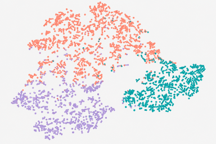
\includegraphics[width=0.45\linewidth]{figure/ACM_clusters.png}
    \caption{t-SNE visualization of learned ACM paper embeddings. Each point represents one paper, and color denotes its class.}
    \label{fig:clustering-acm}
\end{figure}

\begin{figure}[H]
    \centering
    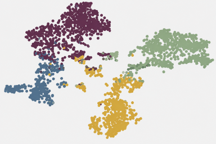
\includegraphics[width=0.45\linewidth]{figure/DBLP_clusters.png}
    \caption{t-SNE visualization of learned DBLP author embeddings. Each point represents one author, and color denotes its research area.}
    \label{fig:clustering-dblp}
\end{figure}

\begin{table}[H]
  \centering
  \caption{Additional clustering-quality diagnostics on DBLP and ACM,
  reported as mean $\pm$ standard deviation over five runs. Best mean
  values are bold.}
  \label{tab:clustering-diagnostic}
  \small
  \resizebox{\columnwidth}{!}{%
  \begin{tabular}{llcccc}
    \toprule
    & & \multicolumn{2}{c}{DBLP} & \multicolumn{2}{c}{ACM} \\
    \cmidrule(lr){3-4}
    \cmidrule(lr){5-6}
    \textbf{Group} & \textbf{Model}
    & NMI & ARI
    & NMI & ARI \\
    \midrule

    Hom./hom.
    & GAT
    & $71.50 \pm 0.36$
    & $77.26 \pm 0.48$
    & $57.22 \pm 0.19$
    & $60.47 \pm 0.31$ \\
    \midrule

    \multirow{2}{*}{Het./hom.}
    & NSD
    & $80.21 \pm 0.62$
    & $84.04 \pm 0.43$
    & $62.56 \pm 0.37$
    & $65.02 \pm 0.28$ \\

    & CSNN
    & $81.72 \pm 0.39$
    & $84.25 \pm 0.55$
    & $69.28 \pm 0.45$
    & $71.10 \pm 0.34$ \\
    \midrule

    \multirow{2}{*}{Hom./het.}
    & HAN
    & $79.12 \pm 0.47$
    & $84.76 \pm 0.58$
    & $60.63 \pm 0.22$
    & $64.28 \pm 0.41$ \\

    & PSHGCN
    & $80.38 \pm 0.52$
    & $82.65 \pm 0.36$
    & $71.89 \pm 0.49$
    & $74.31 \pm 0.57$ \\
    \midrule

    \multirow{2}{*}{Het./het.}
    & Hetero2Net
    & $80.54 \pm 0.33$
    & $84.98 \pm 0.46$
    & $70.14 \pm 0.40$
    & $73.42 \pm 0.51$ \\

    & LatGRL
    & $81.36 \pm 0.56$
    & $86.07 \pm 0.38$
    & $72.52 \pm 0.61$
    & $76.75 \pm 0.44$ \\
    \midrule

    Ours
    & \textbf{\method{}}
    & $\mathbf{82.41 \pm 0.35}$
    & $\mathbf{86.52 \pm 0.42}$
    & $\mathbf{75.78 \pm 0.37}$
    & $\mathbf{78.29 \pm 0.31}$ \\
    \bottomrule
  \end{tabular}
  }
\end{table}

\section{Additional Analysis: Diffusion Process of {\method{}}}
\label{sec:diffusion-process-analysis}

We further inspected the training dynamics of \method{} on a controlled four-class
\texttt{FakeHeteroDataset} from torch geometric library. The model was trained with the default synthetic-data settings, and
the visualization includes only nodes with class labels. We recorded the classified-node embedding
layout every five epochs. As shown in Figure~\ref{fig:fakehetero-diffusion-process}, at the beginning of training, nodes from different classes are strongly interleaved. As training proceeds, same-class nodes gradually move toward compact regions, and the
four class-level groups become increasingly separated. This observation suggests that \method{} effectively learns to diffuse information across the heterogeneous graph structure, leading to improved class separability in the learned embeddings.

 \begin{figure}[H]
   \centering
   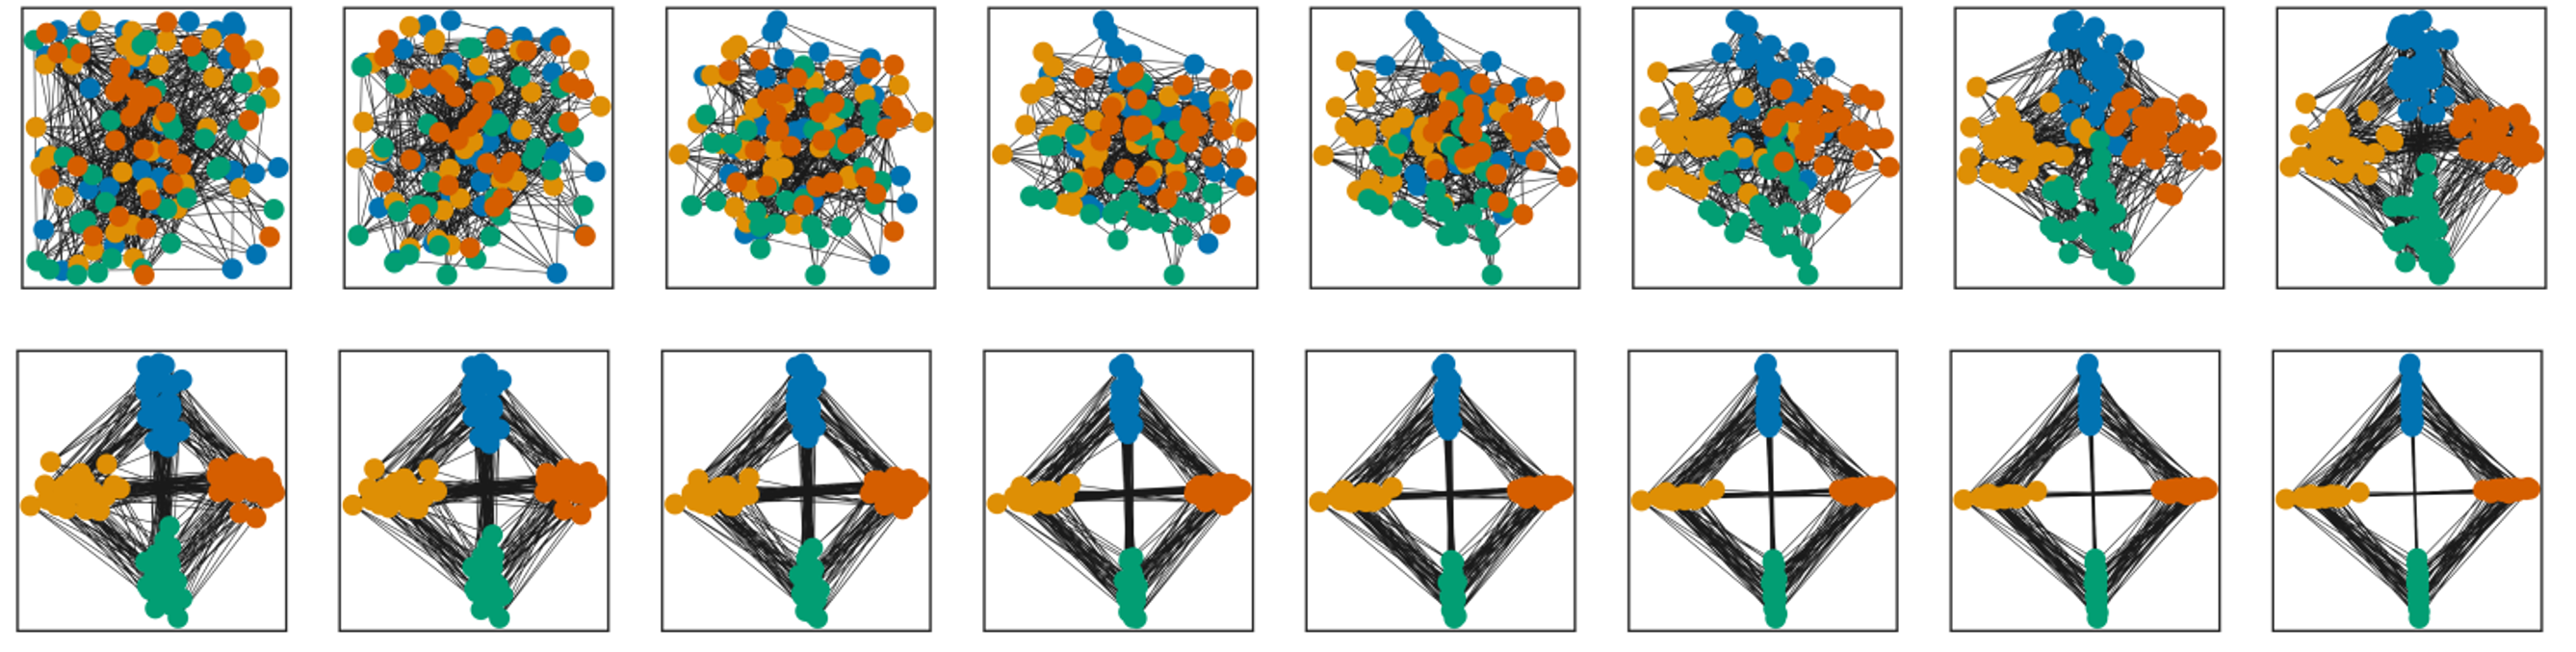
\includegraphics[width=\linewidth]{figure/fakehetero_diffusion_process.png}
   \caption{Training-time diffusion trajectory of \method{} on the four-class
   \texttt{FakeHeteroDataset}. Only labeled nodes are visualized, and consecutive panels are
   separated by five training epochs.}
  \label{fig:fakehetero-diffusion-process}
\end{figure}

\section{Computational Efficiency}

To have a better understanding of the computational cost, we conducted a big-O analysis of \method{}'s, \ampss{}'s, and \sheafconvpool{}'s time and space complexity.

Let $N=|V|$ and
$M=|E|$ be the number of nodes and directed edges, $F$ the number of retained path instances,
and $I=\sum_{f=1}^F \ell_f$ the total edge-face incidences ($\ell_f$ = length of instance
$f$). Let $d$, $d_r$, $d_h$ denote the stalk, relation-embedding, and sequence-encoder
dimensions, and $K$ the number of Hodge-diffusion steps. Because every edge on a retained
path contributes its own edge-to-face restriction map, the upper Hodge term scales with $I$
rather than $F$ alone.

\paragraph{\ampss{} preprocessing.} Schema construction runs once, before training. With $P$
label-propagation steps, $C_y$ classes, $C_\Sigma$ candidate schemas, $S$ retained schemas,
maximum schema length $L$, and $Q_{\mathrm{type}}$, $Q_{\mathrm{path}}$ the number of typed
and concrete path prefixes visited during enumeration and scoring, preprocessing costs
\[
O\!\left(P(M+N)C_y + Q_{\mathrm{type}} + Q_{\mathrm{path}} + \widehat{F}C_y + C_\Sigma S U + I\right)
\]
time and $O\!\left(M+NC_y+C_\Sigma(L+U)+I\right)$ space, where $\widehat{F}$ instances are
sampled for scoring and $U$ bounds a sampled endpoint set. In the worst case
$Q_{\mathrm{type}}=O(Tb_\Sigma^{L})$ and $Q_{\mathrm{path}}=O((C_\Sigma+S)N\bar{d}^{\,L})$;
in practice \ampss{} caps $C_\Sigma$, $S$, and the number of materialized instances, so the
realized cost is output-sensitive rather than exponential. At inference, the schema gates
cost $O(S)$ per forward pass, and the instance gates (MLP width $h_\beta$) add
$O\!\left(F(2d+d_r)h_\beta\right)$ time and $O(F)$ space.

\paragraph{\method{}.} Table~\ref{tab:complexity} summarizes the per-component
cost of a forward pass, with node-to-edge and edge-to-face MLP widths $h_e$, $h_f$, and
$q(d)=O(d^3)$ for the Householder parameterizations we implement ($O(d^2)$ for
unrestricted dense maps).

\begin{table}[h]
\centering
\small
\caption{Per-component time and space complexity of the \method{} model. $K$ is the number of diffusion steps}
\label{tab:complexity}
\begin{tabular}{lll}
\toprule
Component & Time & Space \\
\midrule
Node-to-edge & $M\left[(2d+d_r)h_e+h_ed^2+q(d)\right]$ & $Md^2$ \\
Edge-to-face & $I\left[(2d+d_r)h_f+h_fd_h+d_h^2+d_hd^2\right]$ & $Id^2$ \\
Hodge diffusion & $K(M+I)d^2$ & $(M+I)d^2$ \\
\bottomrule
\end{tabular}
\end{table}

Since node-to-edge and edge-to-face maps are cached and reused across all $K$ diffusion
steps, the full forward pass (excluding readout) costs
\[
O\!\left(Nd_{\mathrm{in}}d + (M+I)d^3 + K(M+I)d^2\right)
\]
once hidden widths scale with $d$, linear in the number of edges and retained edge-face
incidences for fixed $d$. Inference memory is $O\!\left((M+I)d^2+(N+M)d+Id_h\right)$,
dominated by the cached maps; training adds up to $O(K(N+M)d)$ for the diffusion trajectory.

\paragraph{\sheafconvpool{} readout.} With $r=3$ node/edge views, projected-descriptor
dimension $f$, pooling width $h_p$, batch size $G$, and $C$ classes, the readout costs
\[
\begin{array}{@{}l@{}}
O\bigl((N+M)[dr^2+r^2h_p+h_pf+f^2] \\
\qquad{}+G[h_pf^2+h_pC]\bigr)
\end{array}
\]
time and
\[
O\!\left((N+M)(dr+f^2)+Gf^2\right)
\]
space. With $r=3$ and $f=8$ fixed, this reduces to $O((N+M)d)$: a linear-time readout
added on top of the model, with no dense Laplacian, node-node covariance, or coarsened graph
ever built.

Furthermore, we reported measured runtime, parameter count, and memory on the ACM node
classification task in Table~\ref{tab:efficiency}.

\begin{table}[H]
  \centering
  \caption{Efficiency comparison on ACM. Best values are bold. Hetsheaf's code is not available, so we used the Hetsheaf-ensemble model reported results in the original paper.}
  \label{tab:efficiency}
  \small
  \begin{tabular}{lccc}
    \toprule
    \textbf{Model} & Runtime (s) & Parameters & Memory (MB) \\
    \midrule
    R-GCN & \textbf{22.1} & 43M & 1{,}240 \\
    HAN & 28.9 & 2.2M & 1{,}780 \\
    HGT & 1{,}025.8 & 7.2M & 6{,}120 \\
    Sheaf-NSD & 47.6 & \textbf{155K} & \textbf{980} \\
    Hetsheaf & 55.7 & 174K & - \\
    \midrule
    \textbf{\method{}} & 72.1 & 517K & 1120 \\
    \bottomrule
  \end{tabular}
\end{table}

\method{} is not the cheapest model in Table~\ref{tab:efficiency}: R-GCN has the lowest runtime,
and Sheaf-NSD, which models neither relation types nor meta-paths, uses the fewest parameters and
the least memory among the compared models. \method{}'s runtime and parameter count are higher
than Hetsheaf's, the closest heterogeneous sheaf baseline, which we attribute to the additional
edge-to-face maps and \ampss{} schema and instance gates that Hetsheaf does not have. Its memory
footprint nonetheless stays within the same order of magnitude as the other compared models and
well below the heterogeneous transformer baseline HGT, so retaining explicit face-level edge state
does not come at a disproportionate memory cost.

\end{document}



\section{Experiments}
\label{sec:experiments}

We evaluated \method{} with \ampss{} on a range of heterogeneous graph tasks, including node classification, link prediction, and graph classification. On the graph classification task, we also evaluated the single-level \sheafconvpool{} readout.

\subsection{Datasets}
To evaluate the performance of \method{}, we used benchmark heterogeneous graph datasets across three tasks: node classification, graph classification, and link prediction.
On the node classification task, we used three benchmark heterogeneous graph datasets from HGB \cite{lv2021hgb}: DBLP \cite{lv2021hgb} and IMDB \cite{lv2021hgb}, and ACM \cite{wang2019han}. The statistics of these datasets are summarized in Table~\ref{tab:node-datasets} in Appendix~\ref{app:benchmark-datasets}. 

On the graph classification task, we used four benchmark heterogeneous graph datasets from TUDataset \cite{morris2020tudataset}: biological graphs, including PROTEINS and ENZYMES, and chemical compound graphs, including MUTAG and NCI1. To make those graphs heterogeneous, we treated the node and edge labels supplied by TUDataset as different node and edge types. Table~\ref{tab:graph-datasets} in Appendix~\ref{app:benchmark-datasets} gives the statistics of the four TUDataset graph-classification benchmarks.

On the link prediction task, we used four benchmark heterogeneous graph datasets from HGB \cite{lv2021hgb}: user-item interaction networks, including LastFM, YouTube, and Amazon; and a biological knowledge graph, including PubMed. The statistics of these datasets are summarized in Table~\ref{tab:link-datasets} in Appendix~\ref{app:benchmark-datasets}.


\subsection{Baselines}

To evaluate the performance of \method{}, we compared it against a range of state-of-the-art baselines, including homogeneous homophilic models, homogeneous heterophilic models, heterogeneous homophilic models, and heterogeneous heterophilic models.
On the node classification task, we compared \method{} against four groups of baselines: (i) homogeneous homophilic models, including GCN
\cite{kipf2017gcn}, GAT \cite{velickovic2018gat}, and ChebNetII \cite{he2022chebnetii}; (ii) homogeneous heterophilic models, including NSD
\cite{bodnar2022neural} and CSNN \cite{ribeiro2026cooperative}; (iii)
heterogeneous homophilic models, including HAN \cite{wang2019han}, SeHGNN \cite{yang2023sehgnn},
HiNormer \cite{mao2023hinormer}, and PSHGCN \cite{he2024spectral}; and heterogeneous heterophilic models, including HDHGR \cite{guo2023homophily}, Hetero$^2$Net \cite{li2025hetero2net}, H2SGNN
\cite{lu2026addressing}, HetSheaf \cite{braithwaite2024heterogeneous}, and LatGRL
\cite{shen2025heterophily}.

On the graph classification and link prediction tasks, we compared \method{} against four groups of baselines: (i) homogeneous homophilic models, including GCN \cite{kipf2017gcn} and GAT \cite{velickovic2018gat}; (ii) homogeneous heterophilic models, including NSD \cite{bodnar2022neural} and CSNN \cite{ribeiro2026cooperative}; (iii) heterogeneous homophilic models, including HAN \cite{wang2019han} and PSHGCN \cite{he2024spectral}; and (iv) heterogeneous heterophilic models, including HDHGR \cite{guo2023homophily}, Hetero$^2$Net \cite{li2025hetero2net}, H2SGNN \cite{lu2026addressing}, HetSheaf \cite{braithwaite2024heterogeneous}, and LatGRL \cite{shen2025heterophily}.





\subsection{Experiments Settings}

In Tables~\ref{tab:node-cls}, \ref{tab:graph-cls}, and \ref{tab:link-pred}, we group the baselines introduced in each subsection’s \emph{Baselines} paragraph into four categories: Hom./hom., Het./hom., Hom./het., and Het./het. The first term indicates whether the model assumes a homogeneous or heterogeneous graph, while the second indicates whether it is designed for homophilic or heterophilic settings. \method{} is reported separately under Ours. Since HetSheaf does not provide a public implementation, we report the results published in its original paper, which follows the same experimental settings as ours. To ensure a fair comparison, we conducted the experiments with 5 different random seeds and reported the average performance with standard deviation.


In general, the model selection was performed using hyperparameter sweeps. The full per-dataset hyperparameters are listed in Appendix~\ref{app:hyperparameters}. The code is available at \url{placeholder_for_code_repository.com}.

To address these problems, we propose Heterophilic heterogeneous sheaf neural network (\method{}), a heterogeneous heterophilic sheaf-Hodge neural network for heterogeneous heterophilic graphs that treats  meta-path instances as higher-order. We firstly propose a method to model a heterogeneous heterophilic graph with meta-paths as a 2D-cellular graph. Then, we learn both structure via sheaf restriction maps and diffusion, preserving locality which causes heterophily and heterogeneous from graph structure. We further introduce Automatic meta-paths selection for sheaf neural network (\ampss{}) as a subcomponent in \method{}, a two-stage meta-path selection mechanism that learns informative meta-paths with learnable weight for both meta-paths schemas and individual path instances during training. Furthermore, for graph classification task, it requires converting node and edge sheaf states into a single graph-level representation. However, because sheaf neural network uses local vector spaces, this readout should not depend on an arbitrary choice of local basis. For this reason, we introduce Sheaf Covariance Pooling (\sheafcovpool{}) as a graph readout method for \method{}, a gauge-invariant and permutation invariant readout that pools attention-weighted mean and covariance statistics from Gram descriptors of node and edge sheaf states. This produces graph-level representations invariant to \method{}'s orthogonal restriction maps by construction. Together, we propose a framework that ...
\documentclass[sigconf,anonymous,review]{acmart}

\usepackage{amsthm}
\usepackage{algorithm}
\usepackage{algorithmic}
\usepackage{multirow}

\AtBeginDocument{%
  \providecommand\BibTeX{{Bib\TeX}}}

% Replace the ACM metadata below with the values supplied by the proceedings venue.
\setcopyright{acmlicensed}
\copyrightyear{2026}
\acmYear{2026}
\acmDOI{XXXXXXX.XXXXXXX}
\acmConference[Conference acronym 'XX]{ACM Conference}{Month DD-DD, 2026}{City, Country}
\acmISBN{978-1-4503-XXXX-X/2026/MM}

\newcommand{\R}{\mathbb{R}}
\newcommand{\method}{\textsc{H2S-NN}}
\newcommand{\ampss}{\textsc{AMPSS}}
\newcommand{\sheafcovpool}{\textsc{SheafCovPool}}
\newcommand{\cF}{\mathcal{F}}
\newcommand{\cL}{\mathcal{L}}
\newcommand{\norm}[1]{\left\lVert #1\right\rVert}
\newcommand{\transpose}{\mathsf{T}}
\newcommand{\concat}{\mathbin\Vert}
\newtheorem{proposition}{Proposition}

\title[H2S-NN]{H2S-NN: Heterophilic Heterogeneous Neural Networks with Adaptive Meta-Path Selection}

% Replace the affiliation placeholder before submission.
\author{Peeradon Sarnkaew}
\email{peeradonsarnkaew46@gmail.com}
\affiliation{%
  \institution{Independent Researcher}
  \city{Bangkok}
  \country{Thailand}
}
\renewcommand{\shortauthors}{Sarnkaew}

\begin{document}

\begin{abstract}
Heterogeneous graphs contain many node and relation types, and learning on them raises two problems that are usually handled separately but really occur together. Different relation types carry different meanings, so a single shared update rule can blur information that should stay type-aware; and many of these relations are heterophilic, where connected nodes need not share a label or similar features, so a model that assumes neighbors agree can discard the very signal a relation carries. Meta-paths, typed relations such as author-paper-author, are the standard way to expose multi-hop semantics, but existing methods collapse each into a node-to-node view and lose the path structure a heterophily-aware model could act on. We introduce \method{}, which keeps both problems in view. It compares each edge's endpoints in a shared space, so that a relation-aware disagreement rather than a raw feature gap drives learning, and it retains selected meta-path instances as higher-order structure instead of reducing them to endpoint pairs. To avoid hand-picking meta-paths, \ampss{} learns which schemas and instances matter jointly with the task, while \sheafcovpool{} pools the result for graph classification. Across benchmarks, \method{} leads on node and graph classification and stays competitive on link prediction; ablations confirm that each component contributes.
\end{abstract}

\ccsdesc[500]{Computing methodologies~Neural networks}

\keywords{heterogeneous graph neural networks, heterophily, sheaf neural networks, meta-path discovery, graph pooling}

\maketitle

\section{Introduction}
\label{sec:introduction}


Heterogeneous graphs are a common representation for modeling complex relational structures, such as citation 
networks \cite{liu2014meta} or social interactions \cite{singh2025overview}. Unlike homogeneous graphs, heterogeneous graphs contain multiple types of nodes and edges wwith distinct semantic roles \cite{sun2013mining}. Moreover, many graphs are also heterophilic, where nodes may have different properties. A graph can therefore be both heterogeneous and heterophilic, resulting in a much more complex learning task called heterogeneous heterophilic graph learning, as shown in Figure \ref{fig:het_hom_graph}. Furthermore, modeling graphs under the simplifying assumptions of homogeneity or homophily can obscure important structural and relational patterns. This mismatch provides the model with an incomplete representation of the original graph and may consequently degrade predictive performance \cite{lin2025heterophily}. 

\begin{figure}
  \centering
  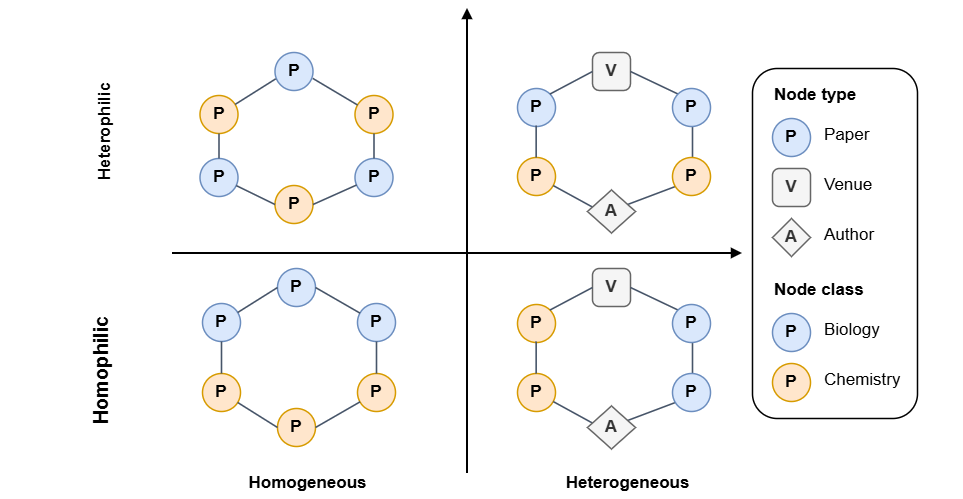
\includegraphics[width=\columnwidth]{figure/Het_HomGraph.drawio.png}
  \caption{An example of heterogeneous heterophilic graph. The graph contains multiple types of nodes and edges, and connected nodes may have different properties.}
  \label{fig:het_hom_graph}
\end{figure}

Many existing methods address either heterogeneous graphs without explicitly considering heterophily \cite{hu2020heterogeneous,mao2023hinormer,he2024spectral,yang2023simple,wang2019heterogeneous,zhang2019heterogeneous} or heterophilic graphs without modeling heterogeneous node and edge types \cite{grover2025spectro,yue2025graph,bodnar2022neural,ribeiro2026cooperative}. Recent methods have begun to address heterogeneous heterophilic graphs through meta-path-based latent subgraphs \cite{lu2026addressing,chen2025adaptive,li2025hetero2net,guo2023homophily,shen2025heterophily,wang2025homophily}, graph rewiring \cite{tao2025cross}, graph transformers \cite{lin2025heterophily}, and sheaf-based mappings \cite{braithwaite2024heterogeneous}. Among these directions, meta-paths can express information that is not contained in either endpoint alone \cite{sun2011pathsim}. For instance, an \texttt{Author-Paper-Author} meta-path describes a co-authorship relation in citation networks, as shown in Figure~\ref{fig:meta_path}. However, existing methods either ignore meta-paths completely, use meta-paths as semantic views, filtered edge sets, or aggregation channels rather than retaining each concrete path instance as part of the propagation structure. For example, an \texttt{A-P-A} meta-path can connect two authors through a shared paper, but after it is converted into an author-author view, the shared paper and the two authorship edges no longer directly shape the propagation operator. This is limiting under heterophily, because whether information should be reinforced or contrasted can depend on the relations along the path, not only on the endpoint connection. This can weaken locality and higher-order information from meta-paths as a part of graph structure.

\begin{figure}
  \centering
  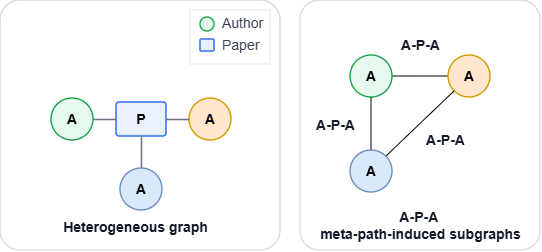
\includegraphics[width=\columnwidth]{figure/meta_path.drawio.png}
  \caption{Illustration of meta-path-induced graph transformation. Under the A-P-A meta-path, authors that share a paper in the original heterogeneous graph are connected in an author-level subgraph.}
  \label{fig:meta_path}
\end{figure}

Manual meta-path specification creates a second bottleneck. Hand-crafted meta-paths are difficult in complex networks, and some useful paths might be ignored \cite{zhong2022pmhgnn,li2024lmsps}. Moreover, datasets often lack such predefined meta-paths. There exists multiple methods for finding useful meta-paths automatically, but they are usually computationally expensive. Some
methods reduce this burden through progressive sampling \cite{li2024lmsps}, searching algorithm \cite{zhang2026mctshgnn,li2023pmmm,li2026amphgnas,sun2025hgsearch}, or reinforcement learning
\cite{zhong2022pmhgnn}.
Although automatic meta-path search reduces reliance on expert knowledge, most methods still select or weight meta-paths at the schema level. However, it is too coarse: a \texttt{PAP} schema may be useful overall, while some concrete \texttt{PAP} instances connect unrelated papers and introduce noise. Schema-level selection must therefore keep noisy instances with useful ones or discard the entire schema. In addition, many search methods select schemas before training the prediction model, so schema choice and instance relevance cannot be refined jointly by the task objective.

To address these challenges, we propose the Heterophilic Heterogeneous Sheaf Neural Network (\method{}), a sheaf–Hodge neural architecture for heterogeneous graphs with heterophily. \method{} represents meta-path instances as higher-order structures by modeling the input graph as a two-dimensional cellular complex. It then learns structural information through sheaf restriction maps and diffusion while preserving the local interactions that give rise to heterophily and heterogeneity.

We further introduce Automatic Meta-Path Selection for Sheaf Neural Networks (\ampss{}), a two-stage component that identifies informative meta-paths during training. \ampss{} learns weights at both the meta-path-schema level and the individual path-instance level.

For graph classification, node and edge sheaf states must be aggregated into a single graph-level representation. Because these states belong to local vector spaces, the readout should be independent of arbitrary choices of local basis. We therefore propose Sheaf Covariance Pooling (\sheafcovpool{}), a gauge- and permutation-invariant readout that aggregates attention-weighted mean and covariance statistics derived from Gram descriptors of node and edge sheaf states. By construction, the resulting graph representation is invariant under the orthogonal transformations associated with \method{}'s restriction maps.

Together, these components form a unified framework for learning meta-paths as higher-order relation in original graphs, heterogeneous, and heterophilic graph representations.




Our main contributions are summarized as follows:
\begin{enumerate}
  \item We introduce \method{}, a heterogeneous sheaf-Hodge framework that retains concrete typed
  path instances as a face-like component on our proposed 2D-cellular graphs, resulting in a learned graph structure that preserves locality without breaking heterophily on heterogeneous graphs.
  \item We propose \ampss{}, a two-stage schema-to-cell selection mechanism that combines
  training-only candidate preselection with differentiable schema- and instance-level refinement
  inside the upper edge Laplacian. This subcomponent allows \method{} to learn which concrete occurrences
  of a schema are useful for the task.
  \item For graph classification, we introduce \sheafcovpool{} as a readout function for graph classification task in \method{}, a gauge-invariant and permutation invariant readout that scores per-node and per-edge learned attention and pools their
  attention-weighted mean and covariance, producing a graph-level representation that is suitable for sheaf neural network.
\end{enumerate}

To this end, we evaluate the framework across node classification, graph classification, and
heterogeneous link prediction. As a result, \method{} achieves the best overall performance across all tasks including node classification, graph classification, and heterogeneous link prediction.

\section{Preliminaries}
\label{sec:background}


\subsection{Heterogeneous graphs}

A heterogeneous graph is a tuple $G=(V,E,\phi,\psi)$, where $V$ and $E$ are the node and edge
sets, $\phi:V\rightarrow\mathcal{T}$ assigns each node a type, and
$\psi:E\rightarrow\mathcal{R}$ assigns each edge a relation type. The realized type sets are
$\mathcal{T}=\{\phi(v):v\in V\}$ and $\mathcal{R}=\{\psi(e):e\in E\}$. The graph is heterogeneous
when it contains more than one node type or more than one relation type, i.e.,
$|\mathcal{T}|>1$ or $|\mathcal{R}|>1$; it reduces to a homogeneous graph when
$|\mathcal{T}|=|\mathcal{R}|=1$ \cite{lu2026addressing}.

\subsection{Homophily and Heterophily}
Homophily describes the tendency of connected nodes to share the same label. For a graph
$G'=(V',E')$ whose endpoint labels are comparable, its edge homophily is
\begin{equation}
  H_{\mathrm{edge}}(G')
  = \frac{1}{|E'|}\sum_{(u,v)\in E'}\mathbf{1}[y_u=y_v],
  \label{eq:background-edge-homophily}
\end{equation}
where $y_u$ is the label of node $u$ and $\mathbf{1}[\cdot]$ is the indicator function
\cite{zhu2020beyond}. Heterophily describes the opposite tendency: adjacent nodes are more likely to have different labels. Larger homophily values indicate stronger label agreement. For heterogeneous graphs, we compute homophily on each meta-path-induced homogeneous subgraph and average across the considered meta-paths \cite{shen2025UHGRL}:
\begin{equation}
    \mathcal{H}
    =
    \frac{1}{|\mathcal{P}|}
    \sum_{p \in \mathcal{P}}
    H_{\mathrm{edge}}(G'_p),
    \label{eq:overall-homophily}
\end{equation}
where $\mathcal{P}$ denotes the set of all considered meta-paths and $G'_p$ is the homogeneous subgraph induced by meta-path $p$.

\subsection{Meta-path}
A meta-path schema of length $\ell$ is a typed relation sequence
\begin{equation}
  \sigma:
  t_0 \xrightarrow{r_1} t_1 \xrightarrow{r_2}\cdots
  \xrightarrow{r_\ell} t_\ell,
  \qquad t_i\in\mathcal{T},\; r_i\in\mathcal{R},
  \label{eq:background-metapath-schema}
\end{equation}
which specifies a composite relation between its endpoint types \cite{sun2011pathsim}. For each
relation $r$, let $A_r\in\{0,1\}^{|V|\times|V|}$ be its adjacency matrix, with
$(A_r)_{uv}=1$ when an edge of type $r$ connects $u$ to $v$. The schema induces the walk-count
matrix
\begin{equation}
  A_\sigma=A_{r_1}A_{r_2}\cdots A_{r_\ell},
  \label{eq:background-metapath-adjacency}
\end{equation}
where $(A_\sigma)_{uv}$ counts the concrete walks from $u$ to $v$ that follow $\sigma$. When
$t_0=t_\ell$, thresholding $A_\sigma$ produces a homogeneous endpoint graph on which
Eq.~\eqref{eq:background-edge-homophily} can be evaluated. For example, the
paper-author-paper schema has $A_{\mathrm{PAP}}=A_{\mathrm{PA}}A_{\mathrm{AP}}$ and connects
papers that share an author. A concrete path instance is an ordered sequence
$f=(v_0,e_1,v_1,\ldots,e_\ell,v_\ell)$ satisfying $\phi(v_i)=t_i$ and $\psi(e_i)=r_i$. Thus,
$\sigma$ describes a type-level pattern, whereas $f$ identifies one occurrence of that pattern in
the observed graph.

\section{Methodology}
\label{sec:method}

\subsection{Problem Formulation}

We study supervised learning on directed heterogeneous graphs under no homophily assumption.  The
input is a graph
\(G=(V,E,\phi,\psi,X^{\mathrm{raw}})\), where
\(\phi:V\rightarrow\mathcal{T}\) assigns node types,
\(\psi:E\rightarrow\mathcal{R}\) assigns relation types, and
\(X^{\mathrm{raw}}=\{x_v^{\mathrm{raw}}\}_{v\in V}\) contains type-dependent node features with
\(x_v^{\mathrm{raw}}\in\R^{d_{\phi(v)}}\).  Because different node types may have different feature
spaces, and because adjacent or path-connected nodes may have different labels or dissimilar
attributes, the learner cannot rely on a shared feature encoder or a homophilic aggregation rule.

In addition to the typed graph, the model is given a pool of meta-path schemas
\(\Sigma\), either supplied manually or selected by \ampss{}.  A schema
\(\sigma=(t_0,r_1,t_1,\ldots,r_\ell,t_\ell)\) specifies a valid typed relation sequence, while
\(f=(v_0,e_1,v_1,\ldots,e_\ell,v_\ell)\) denotes one concrete path instance satisfying
\(\phi(v_i)=t_i\) and \(\psi(e_i)=r_i\).  Let \(\mathcal{I}_\sigma\) be the set of observed
instances of schema \(\sigma\), and let
\(\mathcal{I}_\Sigma=\bigcup_{\sigma\in\Sigma}\mathcal{I}_\sigma\).  Unlike methods that collapse a
meta-path into an endpoint-level homogeneous graph, we retain each
\(f\in\mathcal{I}_\Sigma\) as an ordered face-like support over its path edges.

The learning problem is to construct a predictor
\[
  \hat{y}_s
  =
  g_\theta(s;G,\mathcal{I}_\Sigma),
\]
for a task-specific supervised object \(s\).  For node classification, \(s\) is a target node; for
link prediction, \(s\) is a candidate typed node pair; and for graph classification, \(s\) is an
entire graph.  Given labeled training objects \(\mathcal{S}_{\mathrm{train}}\), the parameters are
learned by minimizing
\[
  \min_\theta
  \frac{1}{|\mathcal{S}_{\mathrm{train}}|}
  \sum_{s\in\mathcal{S}_{\mathrm{train}}}
  \mathcal{L}\!\left(g_\theta(s;G,\mathcal{I}_\Sigma),y_s\right).
\]
Thus, the central challenge is to learn type-aware and relation-aware propagation operators that
can use selected meta-path instances as higher-order structure, while avoiding the assumption that
connected nodes should become similar.

\subsection{Framework Overview}

We introduce \method{}, a Heterophilic Heterogeneous Sheaf--Hodge Neural Network for supervised learning on heterogeneous heterophilic graphs. As illustrated in Figure~\ref{fig}, the \method{} framework comprises four stages. First, the \emph{Data Input} stage prepares typed node features, relations, and training-only diagnostic statistics. Second, \method{} employs its Automatic Meta-Path Selection subcomponent, \ampss{}, to construct a compact pool of meta-path schemas and learn the importance of their corresponding path instances. Third, the selected paths are incorporated into the sheaf--Hodge encoder, which learns node--edge--face geometry through restriction maps and performs diffusion over node and edge cochains. Finally, \method{} applies a task-specific prediction head. Node classification reads the final states of selected target nodes, link prediction scores pairs of final node representations, and graph classification uses the \sheafcovpool{} subcomponent to aggregate node and edge sheaf states into a graph-level representation.

Thus, \ampss{} serves as the meta-path selection mechanism within \method{}, while \sheafcovpool{} serves as its graph-level readout for graph classification. All tasks share the same underlying sheaf--Hodge encoder and learned geometric operators.

\begin{figure*}[t]
  \centering
  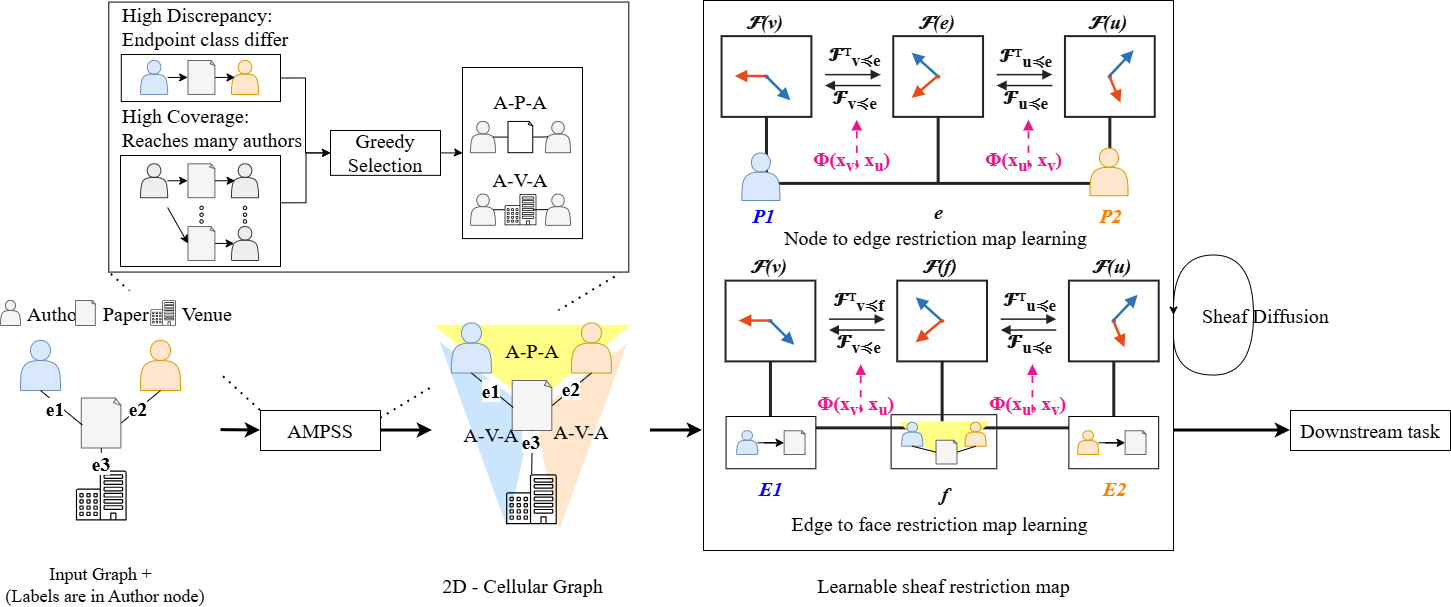
\includegraphics[width=\textwidth]{figure/h2snn_framework_overview.png}
  \caption{Overview of \method{}.  Typed graph data enter a training-only \ampss{} selection stage;
  selected schemas and weighted path instances then parameterize the node-edge-face geometry.
  Node and edge cochains diffuse in parallel before task-specific node, link, or graph prediction,
  with graph classification routed through \sheafcovpool{}.}
  \Description{A left-to-right four-stage diagram.  Data Input feeds AMPSS schema and instance
  selection, which feeds H2S-NN sheaf-Hodge geometry and parallel node and edge diffusion.  The
  output branches to node classification, link prediction, and graph classification through
  SheafCovPool.}
  \label{fig:pipeline}
\end{figure*}



\subsection{Node Stalks and Sheaf Restrictions Initialization}

Firstly, \method{} maps all node types into a shared stalk space and learns relation-aware restrictions
for each typed edge. This is needed because heterogeneous features are not directly comparable since each embedding has a different semantic spaces, and heterophilic edges should measure transported disagreement rather than raw similarity. These
restrictions define the first coboundary \(\delta_0\), which provides the node-to-edge geometry used
by the later edge-to-face construction in cellular sheaves of our \method{}. We therefore map
each type into the common stalk space before comparing adjacent nodes:
\begin{equation}
  h_v^{(0)}
  =\operatorname{Dropout}\!\left[
    \operatorname{GELU}\!\left(
      \operatorname{LN}(W_{\phi(v)}x_v+b_{\phi(v)})+q_{\phi(v)}
    \right)
  \right]\in\R^d ,
  \label{eq:node-encoder}
\end{equation}
where \(W_t,b_t\) are type-specific parameters and \(q_t\) is a learned type embedding.  A learned
node table supplies \(h_v^{(0)}\) when raw attributes are unavailable.  We initialize the diffused
node cochain as \(x^{(0)}=h^{(0)}\), and represent each relation \(r\) by
\(z_r\in\R^{d_r}\).

To ensure Relation-conditioned restrictions, given an oriented edge \(e=(u\xrightarrow{r}v)\), two relation-conditioned networks infer
\(F_{u\unlhd e},F_{v\unlhd e}\in\R^{d\times d}\) from
\(h_u^{(0)}\), \(h_v^{(0)}\), and \(z_r\).  Each restriction is scaled orthogonal:
\begin{equation}
  F_{v\unlhd e}=\lambda_{v,e}Q_{v,e},
  \qquad Q_{v,e}^{\transpose}Q_{v,e}=I,
  \qquad \lambda_{v,e}>0 ,
  \label{eq:conformal-map}
\end{equation}
and analogously for \(F_{u\unlhd e}\).  The orthogonal factor aligns local coordinates, while the
positive scale adjusts the strength of the incidence.  These restrictions define the first
coboundary immediately:
\begin{equation}
  (\delta_0x)_e
  =F_{v\unlhd e}x_v-F_{u\unlhd e}x_u .
  \label{eq:delta0}
\end{equation}
Thus, \(\delta_0x\) measures endpoint disagreement after relation-specific transport rather than
raw feature difference. Then, we initialize the edge cochain with a learnable MLP,
\begin{equation}
  s_e^{(0)}
  =\operatorname{MLP}_{\mathrm{init}}\!\left(
    h_u^{(0)}\concat h_v^{(0)}\concat z_r
    \concat(\delta_0h^{(0)})_e
  \right),
  \label{eq:edge-init}
\end{equation}
so \(s^{(0)}\neq\delta_0h^{(0)}\) in general.  This preserves an edge component outside
\(\operatorname{im}\delta_0\) for the subsequent lower- and upper-Hodge interactions.

\subsection{\ampss{}: Adaptive Meta-Path Schema-to-Cell Selection}
\label{sec:ampss}

\ampss{} separates economical structure search from task-driven refinement.  The first stage is a
non-differentiable, training-only construction of a candidate pool; the second stage learns soft
weights for the retained schemas and their concrete instances jointly with \method{}.

\paragraph{Stage I: candidate generation and preselection.}
The first stage constructs a small set of typed higher-order supports before the neural model is
trained.  It does so at the level of the heterogeneous schema rather than by immediately traversing
all concrete node paths.  We first form a directed type graph whose nodes are entity types and whose
directed edges are relation types, e.g., \(P\xrightarrow{\mathrm{writes}^{-1}}A\) and
\(A\xrightarrow{\mathrm{writes}}P\) in a paper--author network.  A bounded depth-first search over
this type graph enumerates valid schema candidates
\(\sigma=(t_0,r_1,t_1,\ldots,r_\ell,t_\ell)\) subject to the allowed length range and, when
required by the task, the start and end target types.  This step therefore proposes only type-valid
relational routes; it does not yet decide that any route is useful.

For each candidate schema, \ampss{} then samples concrete instances in the original graph.  Starting
from nodes of type \(t_0\), it follows the prescribed relation sequence
\((r_1,\ldots,r_\ell)\) and records paths
\(f=(v_0,e_1,v_1,\ldots,e_\ell,v_\ell)\) whose node and edge types match the schema.  Separate
budgets cap the number of candidate schemas, the number of instances expanded from one anchor node,
the number of instances retained for one schema, and the total number of materialized instances.
These caps make the construction economical while still exposing the model to the main typed
relational patterns present in the graph.

The preselection score is designed to keep schemas that are both informative and usable as
face-like supports.  For node classification, training labels are propagated for a fixed number of
steps to obtain soft endpoint distributions \(\widehat y_v\).  A concrete path receives a large
discrepancy when its two endpoints carry different training-derived class evidence, and a schema
receives the average discrepancy of its sampled instances:
\begin{equation}
  d(f)=\norm{\widehat y_{v_0}-\widehat y_{v_\ell}}_2^2,
  \qquad
  D(\sigma)=\frac{1}{|\mathcal{I}_{\sigma}|}
  \sum_{f\in\mathcal{I}_{\sigma}}d(f).
  \label{eq:discrepancy}
\end{equation}
Intuitively, this favors schemas whose endpoints expose nontrivial class contrast under the
training signal, which can create useful edge-level disagreement for the subsequent Hodge diffusion.
For link prediction, the same idea is implemented with two propagated endpoint-role channels that
mark source and target positions using training-positive edges only.  Neither validation nor test
labels or links contribute to these statistics.

For graph classification, endpoint discrepancy is not the relevant signal.  Let
\(n_{\sigma,c}^{\mathrm{pres}}\) be the number of training graphs of class \(c\) in which schema
\(\sigma\) occurs, \(N_c\) the number of training graphs in that class, and \(n_\sigma\) the total
number of its materialized instances.  The presence score is
\begin{equation}
  P_G(\sigma)
  =\operatorname{Var}_{c}\!\left(
    \frac{n_{\sigma,c}^{\mathrm{pres}}}{\max(N_c,1)}
  \right)+10^{-3}\log(1+n_\sigma).
  \label{eq:graph-presence-score}
\end{equation}
This favors schemas whose presence differs across training classes, with frequency used only as a
small tie breaker.

For node and link tasks, \ampss{} greedily builds the selected pool one schema at a time.  The
score combines four quantities.  The discrepancy \(D(\sigma)\) measures task relevance.  The
endpoint coverage \(C(\sigma)\) measures how many target-type endpoints are reached by the sampled
instances, so a schema that appears only in a tiny corner of the graph is not selected merely
because it has a high local score.  The type diversity \(V(\sigma)\) rewards schemas that pass
through multiple semantic types rather than repeatedly using the same type pattern.  Finally,
\(J(\sigma,\sigma')\) measures endpoint-set overlap with an already selected schema
\(\sigma'\), discouraging several selected schemas from describing nearly the same region of the
graph.  Given the current pool \(S\), the greedy score is
\begin{equation}
  q(\sigma\mid S)=
  \frac{D(\sigma)^{a_d}C(\sigma)^{a_c}V(\sigma)^{a_v}}
       {1+\max_{\sigma'\in S}J(\sigma,\sigma')} ,
  \label{eq:topology-score}
\end{equation}
The numerator prefers schemas that are informative, sufficiently covered, and semantically varied;
the denominator lowers the priority of schemas that are redundant with the pool already chosen.
Graph tasks use the class-presence score \(P_G(\sigma)\) instead of Equation~\ref{eq:topology-score}.
After this greedy pass, the selected schemas are materialized as ordered path supports, together
with the closure pairs used by the node-side correction.  This entire stage fixes the candidate
support and is intentionally non-differentiable; the next stage decides how strongly the retained
schemas and their individual instances should participate in the learned operator.

\paragraph{Stage II: differentiable schema and instance refinement.}
Preselection decides what can be considered; it does not force every retained structure to
contribute equally.  We learn one gate per schema and a state-dependent gate for every path
instance:
\begin{equation}
  \begin{aligned}
  \alpha_\sigma&=\operatorname{sigmoid}(\theta_\sigma),\\
  \beta_f&=\operatorname{sigmoid}\!\left(
    g_\beta(h_{v_0}^{(0)}\concat h_{v_\ell}^{(0)}\concat e_\sigma)
  \right),\\
  w_f&=\alpha_{\sigma(f)}\beta_f .
  \end{aligned}
  \label{eq:gates}
\end{equation}
Here \(e_\sigma\) is a learned schema embedding.  Schema logits are warm-started from standardized
preselection scores, while \(\beta_f\) lets two instances of the same schema have different
effects.  During training, partial-schema propagation retains each schema with probability
\(p_{\mathrm{keep}}\) and rescales a retained gate by \(1/p_{\mathrm{keep}}\), following the
stabilization idea of partial message propagation \cite{li2023pmmm}.

The discovery loss applies complementary pressures rather than a single hard selection rule:
\begin{equation}
  \begin{aligned}
  \cL_{\mathrm{disc}}={}&
  \lambda_s\cL_{\mathrm{sparse\text{-}schema}}
  +\lambda_i\cL_{\mathrm{sparse\text{-}instance}}
  +\lambda_r\cL_{\mathrm{redundancy}}\\
  &+\lambda_v\cL_{\mathrm{coverage}}
  +\lambda_{\mathrm{cost}}\cL_{\mathrm{cost}}
  +\lambda_H\cL_{\mathrm{entropy}} .
  \end{aligned}
  \label{eq:discovery-loss}
\end{equation}
Schema and instance terms discourage diffuse activation; redundancy penalizes similar active
coverage profiles; the negative coverage reward discourages a trivial empty pool; cost suppresses
long, frequently instantiated schemas; and entropy minimization sharpens schema decisions.  These
terms refine only the preselected pool and do not make candidate generation differentiable.

\begin{algorithm}[t]
  \caption{\ampss{} candidate preselection and differentiable refinement}
  \label{alg:ampss}
  \begin{algorithmic}[1]
    \REQUIRE Typed relation graph, training split, schema and instance budgets
    \STATE \textbf{Stage I: Candidate generation and training-only preselection}
    \STATE Enumerate bounded typed schemas and sample concrete instances
    \STATE Compute node/link discrepancy scores or graph presence scores
    \STATE Greedily retain a compact pool \(\Sigma\) and materialize its path supports
    \STATE Initialize \(\theta_\sigma\) from standardized preselection scores
    \FOR{each training epoch}
      \STATE \textbf{Stage II: Differentiable schema and instance refinement}
      \STATE Use uniform face weights during warm-up
      \STATE Compute \(\alpha_\sigma\), \(\beta_f\), and \(w_f=\alpha_{\sigma(f)}\beta_f\)
      \STATE Apply partial-schema propagation with keep probability \(p_{\mathrm{keep}}\)
      \STATE Run matrix-free sheaf-Hodge diffusion and the task readout
      \STATE Optimize Equation~\ref{eq:loss}
    \ENDFOR
  \end{algorithmic}
\end{algorithm}

\subsection{2D-cellular Sheaf-Hodge Geometry Construction}

The sheaf-Hodge encoder begins by deciding what the cells of the operator are.  A graph is already
a \(1\)-dimensional cellular complex: nodes are \(0\)-cells and typed edges are \(1\)-cells.
\method{} extends this complex with the selected meta-path instances from \ampss{}.  A concrete
instance
\[
  f=(v_0,e_1,v_1,\ldots,e_\ell,v_\ell)
\]
is treated as a face-like \(2\)-cell supported on its ordered path edges.  Since an open path is not
itself the boundary of a \(2\)-cell, the model also attaches one closure \(1\)-cell
\(e_{\mathrm{cl}}=(v_\ell\rightarrow v_0)\).  The boundary used by the upper Hodge term is then
\[
  \partial f=(e_1,\ldots,e_\ell,e_{\mathrm{cl}}).
\]
This construction keeps the intermediate nodes and relations visible to the operator, instead of
turning the meta-path into a shortcut edge between \(v_0\) and \(v_\ell\).

We write \(\sigma\unlhd\tau\) when a lower-dimensional cell \(\sigma\) is incident to a
higher-dimensional cell \(\tau\).  A cellular sheaf \(\cF\) equips each cell with a local vector
space, or \emph{stalk}, and assigns a linear restriction map
\(F_{\sigma\unlhd\tau}:\cF(\sigma)\rightarrow\cF(\tau)\) to every incidence.  In \method{}, node,
edge, and face stalks all have dimension \(d\).  The node cochain space and the extended edge
cochain space are
\begin{equation}
  C^0(\cF)=\bigoplus_{v\in V}\cF(v),
  \qquad
  C^1(\cF)=\bigoplus_{e\in E\cup E_{\mathrm{cl}}}\cF(e),
\end{equation}
where \(E_{\mathrm{cl}}\) denotes all closure \(1\)-cells.  The selected path instances form the
face cochain space
\begin{equation}
  C^2(\cF)=\bigoplus_{f\in\mathcal{I}_{\Sigma}}\cF(f).
\end{equation}

The node-to-edge restrictions from the previous subsection give the first coboundary
\(\delta_0:C^0(\cF)\rightarrow C^1(\cF)\).  For an oriented edge \(e=(u\rightarrow v)\),
\begin{equation}
  (\delta_0x)_e
  =
  F_{v\unlhd e}x_v-F_{u\unlhd e}x_u .
  \label{eq:background-delta0}
\end{equation}
Thus \(\delta_0x\) is not a homophilic average.  It is a transported endpoint disagreement, and it
is the edge-level signal from which the later Hodge operator can preserve or suppress
heterophilic variation.  What remains is to define the maps from boundary edges into each selected
face so that the resulting second coboundary is compatible with this first one.

\subsection{Path-Supported Edge-Face Geometry}
\label{sec:face-geometry}

The edge-face construction is the step that turns a selected path instance into an operator on edge
states.  For a selected \(P\!-\!A\!-\!P\) instance, the two path edges remain two boundary edges of
one face-like support.  For a general instance
\(f=(v_0,e_1,v_1,\ldots,e_\ell,v_\ell)\), \method{} first learns a single free map \(A_f\) from the
ordered path.  This map fixes the face stalk's frame for that instance; the individual
edge-to-face maps are then derived from \(A_f\) and the already learned node-to-edge restrictions.

Every face group materializes one schema, so all instances in the group have the same length
\(\ell\) and the same relation sequence \((r_1,\ldots,r_\ell)\).  What varies across instances is
the ordered tuple of node states.  The default face encoder therefore concatenates the node states
in path order together with the schema's relation embeddings and applies one network per length:
\begin{equation}
  A_f
  =\operatorname{reshape}\!\Big(
    \operatorname{MLP}_{\ell}\big(
      h_{v_0}^{(0)}\concat\cdots\concat h_{v_\ell}^{(0)}
      \concat z_{r_1}\concat\cdots\concat z_{r_\ell}
    \big),\,d,d\Big).
  \label{eq:face-map}
\end{equation}
Position is preserved by construction: each slot of the concatenation has its own parameters, so
\(A_f\) distinguishes \((v_0,\ldots,v_\ell)\) from any reordering of it.  Because
\(\operatorname{MLP}_\ell\) is shared across all schemas of length \(\ell\), the parameter count
does not grow with the number of selected schemas.  Crucially, \(A_f\) is one map for the whole
instance.  It does not independently rescale the boundary edges.

The reason is structural.  The upper Hodge term should measure edge curl around a selected path
support, not create curl from a pure node gradient.  Therefore the edge-to-face maps cannot be
arbitrary outputs of separate networks.  They must compose with the node-to-edge restrictions below
them.  \method{} enforces this by carrying a transport to the base vertex \(v_0\) along the path:
\begin{equation}
  \begin{aligned}
  T_{v_0}&=A_f,
  \qquad
  T_{v_i}=T_{v_{i-1}}F_{u\unlhd e_i}^{-1}F_{v\unlhd e_i},\\
  F_{e_i\unlhd f}&=T_{v_{i-1}}F_{u\unlhd e_i}^{-1},
  \end{aligned}
  \label{eq:transport}
\end{equation}
where \(u=v_{i-1}\) and \(v=v_i\) are the endpoints of \(e_i\).  The inverse is available in closed
form: by Eq.~\eqref{eq:conformal-map} each map is a positive scale times an orthogonal factor, so
\(F^{-1}=F^{\transpose}/\lambda^2\), and no linear solve is required.  Each
\(F_{e_i\unlhd f}\) transports the \(i\)-th edge state into the face stalk, but it is tied to the
node-edge geometry through the transport recursion.

The closure edge is also defined from this transport rather than learned from another relation
network:
\begin{equation}
  F_{v_0\unlhd e_{\mathrm{cl}}}=I,
  \qquad
  F_{v_\ell\unlhd e_{\mathrm{cl}}}=T_{v_0}^{-1}T_{v_\ell},
  \qquad
  F_{e_{\mathrm{cl}}\unlhd f}=A_f .
  \label{eq:closure-maps}
\end{equation}
The middle map is the path holonomy
\(\prod_i F_{u\unlhd e_i}^{-1}F_{v\unlhd e_i}\), so it is independent of \(A_f\) and adds no
parameters.  The closure cell is therefore a bookkeeping edge that makes ``walk along the path and
return'' a well-defined boundary cycle.  It is not a claim that the endpoints have an observed
relation.

Let \(\eta(e,f)\in\{-1,+1\}\) be the stored incidence orientation.  The face gate enters the
weighted second coboundary:
\begin{equation}
  (\delta_{1,w}s)_f
  =\sqrt{w_f}\sum_{e\in\partial f}
    \eta(e,f)F_{e\unlhd f}s_e .
  \label{eq:delta1}
\end{equation}
Writing
\(B_fs=\sum_{e\in\partial f}\eta(e,f)F_{e\unlhd f}s_e\), its upper-Hodge
contribution is therefore
\begin{equation}
  \delta_{1,w}^{\transpose}\delta_{1,w}
  =\sum_{\sigma\in\Sigma}\sum_{f\in\mathcal{I}_{\sigma}}
    w_f B_f^{\transpose}B_f .
  \label{eq:weighted-up}
\end{equation}
The square root is important: it makes each face contribute linearly in \(w_f\), not quadratically.

An open path is not the boundary of a \(2\)-cell: a cell is attached along a cycle.  Each instance
therefore also carries a synthetic closure \(1\)-cell \(e_{\mathrm{cl}}=(v_\ell\rightarrow v_0)\),
oriented along the cycle, which completes \(\partial f=(e_1,\ldots,e_\ell,e_{\mathrm{cl}})\).  It is a
stateful edge with its own stalk, and its restriction maps are \emph{defined} rather than learned:
\begin{equation}
  F_{v_0\unlhd e_{\mathrm{cl}}}=I,
  \qquad
  F_{v_\ell\unlhd e_{\mathrm{cl}}}=T_{v_0}^{-1}T_{v_\ell},
  \qquad
  F_{e_{\mathrm{cl}}\unlhd f}=A_f .
  \label{eq:closure-maps}
\end{equation}
The middle map reduces to \(\prod_i F_{u\unlhd e_i}^{-1}F_{v\unlhd e_i}\), the holonomy of the path
itself: it is independent of \(A_f\) and adds no parameters.  The closure cell is thus a bookkeeping
device that makes ``traverse this path and return'' well posed, not an asserted relation between the
endpoints.  Figure~\ref{fig:sheaf-hodge-operator} makes this boundary explicit.

\begin{proposition}[Exact cochain condition]
\label{prop:chain}
For every instance whose node sequence is a simple path, the maps of
Eqs.~\eqref{eq:transport}--\eqref{eq:closure-maps} satisfy
\(\delta_{1,w}\delta_0=0\) identically, for every node cochain and every value of the learned
parameters, with no assumption that the sheaf has trivial holonomy.
\end{proposition}

\begin{proof}
By construction \(F_{e_i\unlhd f}F_{u\unlhd e_i}=T_{v_{i-1}}\) and
\(F_{e_i\unlhd f}F_{v\unlhd e_i}=T_{v_i}\), so the \(i\)-th boundary term of \(\delta_{1,w}\delta_0x\)
equals \(T_{v_i}x_{v_i}-T_{v_{i-1}}x_{v_{i-1}}\), and summing over the path telescopes to
\(T_{v_\ell}x_{v_\ell}-T_{v_0}x_{v_0}\).  Eq.~\eqref{eq:closure-maps} gives
\(F_{e_{\mathrm{cl}}\unlhd f}F_{v_0\unlhd e_{\mathrm{cl}}}=T_{v_0}\) and
\(F_{e_{\mathrm{cl}}\unlhd f}F_{v_\ell\unlhd e_{\mathrm{cl}}}=T_{v_\ell}\), so the closure term
contributes \(T_{v_0}x_{v_0}-T_{v_\ell}x_{v_\ell}\) and the total vanishes.  Simplicity is required
because the transport assigns one map per node position; a revisited node — including a coincident
endpoint pair — would be assigned two values.
\end{proof}

\noindent Empirically the residual \(\norm{\delta_{1,w}\delta_0h^{(0)}}/\norm{\delta_0h^{(0)}}\) is
at the level of single-precision roundoff (\(\sim\!10^{-7}\)) on all evaluated datasets, for both
manual and \ampss{} schema sets.

\begin{figure}[t]
  \centering
  \fbox{\rule{0pt}{4.2cm}\rule{0.94\columnwidth}{0pt}}
  %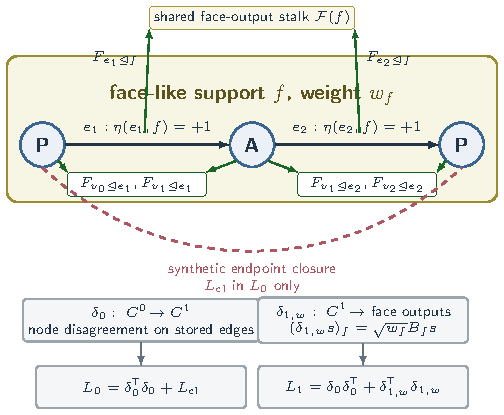
\includegraphics[width=\columnwidth]{figure/h2snn_sheaf_hodge_operator.pdf}
  \caption{AMPSS-selected path instances define a sheaf-Hodge operator. Currently in construction.}
  \label{fig:sheaf-hodge-operator}
\end{figure}

\subsection{Matrix-Free Sheaf-Hodge Diffusion}
\label{sec:closure}

The two coboundaries induce one node operator and one edge operator:
\begin{align}
  L_0x
  &=\delta_0^{\transpose}\delta_0x,
  \label{eq:l0}\\
  L_1s
  &=\underbrace{\delta_0\delta_0^{\transpose}s}_{\text{lower edge term}}
    +\underbrace{\delta_{1,w}^{\transpose}\delta_{1,w}s}_{\text{upper edge term}} .
  \label{eq:l1}
\end{align}
The lower edge term compares edge signals through their incident nodes; the upper term couples the
edges of a boundary cycle through their shared face.  Because the closure \(1\)-cell of
Section~\ref{sec:face-geometry} is an ordinary member of the edge set, it enters \(\delta_0\) — and hence
\(L_0\) and the lower edge term — exactly like a data edge; no separate node-side correction is
applied.  Its restriction maps are the path holonomy of Eq.~\eqref{eq:transport}, so it introduces
no parameters of its own, and a scale \(\gamma>0\) on them is absorbed by the compensating factor in
\(F_{e_{\mathrm{cl}}\lhd f}\), leaving Proposition~\ref{prop:chain} unaffected while tuning how
strongly the boundary cycle closes at the node level.

Starting from \(x^{(0)}=h^{(0)}\) and the independent \(s^{(0)}\), \(K\) explicit Euler steps give
\begin{equation}
  \begin{aligned}
  x^{(k+1)}&=x^{(k)}-\eta_0L_0x^{(k)},\\
  s^{(k+1)}&=s^{(k)}-\eta_1L_1s^{(k)},
  \qquad k=0,\ldots,K-1 .
  \end{aligned}
  \label{eq:diffusion}
\end{equation}
The positive step sizes may be learned.  Node and edge cochains evolve in parallel under geometry
inferred from the same initial node states; there is no cross-rank recurrence between Euler steps.
Layer normalization yields the terminal states \(x^\star\) and \(s^\star\).

Execution is matrix-free: the model applies restrictions in batches and aggregates incident
contributions, without materializing global \(Nd\times Nd\) or \(Md\times Md\) matrices.  Three
implementation boundaries remain consequential.  First, \(\delta_{1,w}\) spans the complete boundary
cycle: the \(\ell\) path edges together with the closure \(1\)-cell.  Second, signed incidences are
supported, and the uniform \(+1\) used here is the correct boundary map precisely because
enumeration traverses every edge along its stored direction and stores the closure cell oriented
along the cycle; the pipeline asserts this rather than assuming it, so a future change to reverse
traversal fails loudly instead of silently invalidating the signs.  Third, because faces must be
simple paths for the transport of Eq.~\eqref{eq:transport} to be well defined, instances that revisit
a node — including those whose endpoints coincide — are excluded during enumeration.  On the
manual meta-path templates this removes a negligible fraction of instances, since the search
backfills its per-anchor budget with simple paths.  Unlike earlier path-supported sheaf
constructions, \(\delta_{1,w}\delta_0=0\) is not encouraged by a penalty but holds identically
(Proposition~\ref{prop:chain}).



\subsection{\sheafcovpool{}}

In sheaf neural diffusion, each node stores its embedding in its own local coordinate system, so embeddings from different nodes cannot simply be pooled together. We therefore introduce \sheafcovpool{}, a readout function that combines node and edge information into a single graph embedding while ignoring these arbitrary coordinate choices. As a result, the graph representation captures the meaningful relationships encoded in \(x^\star\), \(h^{(0)}\), and \(s^\star\), ensuring that the final graph representation reflects the underlying structural information, not the specific basis used to represent each embedding.

The readout first forms small view stacks for nodes and edges.  For a node \(v\), the three views
are its diffused node state, its initial typed state, and the mean state of incident edges.  For an
edge \(e\), the views are the post-diffusion node-to-edge disagreement, the initial disagreement,
and the diffused edge state:
\begin{equation}
  \begin{aligned}
  Z_v^{(0)}
  &=\begin{bmatrix}x_v^\star&h_v^{(0)}&\bar s_v^\star\end{bmatrix}
    \in\R^{d\times3},\\
  Z_e^{(1)}
  &=\begin{bmatrix}
    (\delta_0x^\star)_e&(\delta_0h^{(0)})_e&s_e^\star
  \end{bmatrix}
    \in\R^{d\times3}.
  \end{aligned}
\end{equation}
The Gram descriptor
\[
  G_i^{(r)}=(Z_i^{(r)})^{\transpose}Z_i^{(r)}\in\R^{3\times3},
  \qquad r\in\{0,1\},
\]
records only inner products among these views.  If a local orthogonal gauge changes coordinates as
\(Z_i^{(r)}\mapsto Q_iZ_i^{(r)}\), then \(G_i^{(r)}\) is unchanged.  Thus the classifier sees, for
example, how strongly a node's final state aligns with its initial state or with its incident-edge
summary, but not the arbitrary orientation of the stalk basis.

Nodes and edges play different roles, so separate networks project their descriptors:
\(u_i^{(r)}=\rho_r(\operatorname{vec}G_i^{(r)})\in\R^{d_p}\).  A learned score then selects which
nodes or edges are most informative inside graph \(g\), while the per-graph softmax keeps the
summary permutation invariant:
\begin{equation}
  a_i^{(r)}
  =\frac{\exp(g_r(u_i^{(r)}))}
         {\sum_{j\in\mathcal{C}_r(g)}\exp(g_r(u_j^{(r)}))},
  \qquad
  \mu_r(g)=\sum_{i\in\mathcal{C}_r(g)}a_i^{(r)}u_i^{(r)} .
\end{equation}
Here \(\mathcal{C}_0(g)\) and \(\mathcal{C}_1(g)\) are the nodes and edges of \(g\).  The weighted
mean tells what evidence is present on average, but not whether that evidence is uniform or
concentrated in a few parts of the graph.  \sheafcovpool{} therefore also keeps a weighted
covariance:
\begin{equation}
  \Sigma_r(g)
  =\sum_{i\in\mathcal{C}_r(g)}a_i^{(r)}
    (u_i^{(r)}-\mu_r(g))(u_i^{(r)}-\mu_r(g))^{\transpose}.
\end{equation}
Finally, the graph MLP consumes
\begin{equation}
  \gamma_g=
  \bigl[
  \mu_0(g)\concat\operatorname{triu}(\Sigma_0(g))
  \concat\mu_1(g)\concat\operatorname{triu}(\Sigma_1(g))
  \bigr].
\end{equation}
The result is a single-level readout that uses node and edge evidence, preserves first- and
second-order graph statistics, and remains invariant to node/edge order and orthogonal stalk gauges.

\begin{figure}[t]
  \centering
  \fbox{\rule{0pt}{4.2cm}\rule{0.94\columnwidth}{0pt}}
  %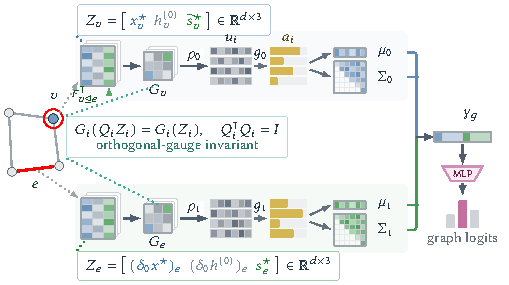
\includegraphics[width=\columnwidth]{figure/sheafcovpool_architecture.pdf}
  \caption{\sheafcovpool{} graph readout. Node and edge view stacks become
  gauge-invariant Gram descriptors; separate attention weights their first and second moments
  before graph classification.}
  \Description{Two parallel node and edge branches.  Each starts with three stalk-valued views,
  forms a Gram descriptor, applies a learned projection and invariant attention, and computes a
  weighted mean and covariance.  Upper-triangular covariance vectors join the means, and the two
  branches concatenate before an MLP outputs graph logits.}
  \label{fig:sheafcovpool}
\end{figure}

\subsection{Training Objective}

\method{} is trained with the supervised task loss and, in auto-discovery mode, the scheduled
\ampss{} discovery objective:
\begin{equation}
  \cL
  =\cL_{\mathrm{task}}
   +\rho(t)\cL_{\mathrm{disc}} .
  \label{eq:loss}
\end{equation}
Here \(\cL_{\mathrm{task}}\) is the task-specific loss, cross-entropy for single-label node and graph classification, and
binary cross-entropy for multi-label classification or link prediction. The \(\cL_{\mathrm{disc}}\) loss combines
the schema- and instance-level gate regularizers used by \ampss{}. The time-dependent coefficient \(\rho(t)\) keeps the discovery regularizers inactive during warm-up and then increases their influence, so the model can first learn task-relevant signals before the \ampss{} discovery process to make the model learn the task first, prevent the discovery process from being collapsed too early.



\section{Experiments}
\label{sec:experiments}


Model selection was performed using hyperparameter sweeps, and the full per-dataset hyperparameters are listed in Appendix~\ref{app:hyperparameters}. To ensure a fair comparison, we ran each experiment with five random seeds and report the mean performance with standard deviation. The code is available at \url{placeholder_for_code_repository.com}. Results for node classification, link prediction, and graph classification are reported in Tables~\ref{tab:node-cls}, \ref{tab:link-pred}, and~\ref{tab:graph-cls}, respectively. Baselines are grouped by graph type and homophily assumption: Hom./hom., Het./hom., Hom./het., and Het./het., where the first term denotes whether the graph is treated as homogeneous or heterogeneous, and the second denotes whether the method targets homophilic or heterophilic settings.

\subsection{Node Classification}
\label{sec:setup-node}


\paragraph{Datasets.}
On the node classification task, we used three benchmark heterogeneous graph datasets: DBLP \cite{lv2021hgb} and IMDB \cite{lv2021hgb}, and ACM \cite{wang2019han}. The statistics of these datasets are summarized in Table~\ref{tab:node-datasets} given in
Appendix~\ref{app:benchmark-datasets}.


\paragraph{Baselines.} We compared \method{} against four groups of baselines: (i) homogeneous homophilic models, including GCN
\cite{kipf2017gcn}, GAT \cite{velickovic2018gat}, and ChebNetII \cite{he2022chebnetii}; (ii) homogeneous heterophilic models, including NSD
\cite{bodnar2022neural} and CSNN \cite{ribeiro2026cooperative}; (iii)
heterogeneous homophilic models, including HAN \cite{wang2019han}, SeHGNN \cite{yang2023sehgnn},
HiNormer \cite{mao2023hinormer}, and PSHGCN \cite{he2024spectral}; and heterogeneous heterophilic models, including HDHGR \cite{guo2023homophily}, Hetero$^2$Net \cite{li2025hetero2net}, H2SGNN
\cite{lu2026addressing}, HetSheaf \cite{braithwaite2024heterogeneous}, and LatGRL
\cite{shen2025heterophily}.


\paragraph{Evaluation Settings.} We followed the HGB benchmark \cite{lv2021hgb} by using the training/validation/test splits in a ratio of 20\%/20\%/60\% on transductive learning. We used Macro-F1 and Micro-F1 as the evaluation metrics.

\paragraph{Results.}
From the results in Table~\ref{tab:node-cls}, \method{} achieved the best performance on all three benchmark datasets in node classification tasks. \method{} outperforms every baselines in every dataset and every setting. This demonstrates the effectiveness of \method{} in capturing complex heterogeneous graph structures and relationships, leading to improved node classification performance.

\begin{table*}[t]
  \centering
  \caption{Performance on node classification benchmarks reporting in Macro-F1 and Micro-F1. Best values are bold.}
  \label{tab:node-cls}
  \scriptsize
  \resizebox{0.8\textwidth}{!}{%
  \begin{tabular}{llcccccc}
    \toprule
    & &
    \multicolumn{2}{c}{DBLP (59.76)} &
    \multicolumn{2}{c}{ACM (72.39)} &
    \multicolumn{2}{c}{IMDB (50.04)} \\
    \cmidrule(lr){3-4}
    \cmidrule(lr){5-6}
    \cmidrule(lr){7-8}
    \textbf{Group} & \textbf{Model}
    & Macro & Micro
    & Macro & Micro
    & Macro & Micro \\
    \midrule

    \multirow{3}{*}{Hom./hom.}
    & GCN
    & $90.77 \pm 0.76$
    & $90.28 \pm 0.20$
    & $91.63 \pm 0.44$
    & $91.38 \pm 0.39$
    & $62.33 \pm 0.58$
    & $67.69 \pm 0.59$ \\

    & GAT
    & $94.39 \pm 1.03$
    & $92.52 \pm 0.27$
    & $92.07 \pm 0.57$
    & $90.71 \pm 0.21$
    & $62.13 \pm 0.26$
    & $68.09 \pm 0.48$ \\
    
    & ChebNetII
    & $92.89 \pm 1.07$
    & $92.67 \pm 0.50$
    & $91.70 \pm 0.27$
    & $91.59 \pm 0.27$
    & $62.97 \pm 0.66$
    & $68.47 \pm 0.55$ \\

    \midrule

    \multirow{2}{*}{Het./hom.}
    & NSD
    & $92.96 \pm 0.21$
    & $93.42 \pm 0.37$
    & $92.33 \pm 0.78$
    & $92.05 \pm 0.69$
    & $61.61 \pm 0.26$
    & $65.23 \pm 0.51$ \\


    & CSNN
    & $93.73 \pm 0.95$
    & $92.12 \pm 0.19$
    & $93.13 \pm 0.94$
    & $92.81 \pm 0.83$
    & $62.92 \pm 0.34$
    & $62.59 \pm 0.22$ \\


    \midrule

    \multirow{4}{*}{Hom./het.}
    & HAN
    & $91.78 \pm 0.92$
    & $92.24 \pm 0.86$
    & $90.88 \pm 0.67$
    & $91.61 \pm 1.07$
    & $61.95 \pm 0.36$
    & $67.76 \pm 0.51$ \\

    & SeHGNN
    & $95.52 \pm 0.98$
    & $95.48 \pm 0.78$
    & $94.38 \pm 1.00$
    & $94.04 \pm 0.73$
    & $72.01 \pm 0.65$
    & $72.59 \pm 0.18$ \\

    & HiNormer
    & $94.06 \pm 0.40$
    & $94.14 \pm 0.46$
    & $91.87 \pm 0.26$
    & $89.64 \pm 0.39$
    & $64.13 \pm 0.19$
    & $67.53 \pm 0.32$ \\

    & PSHGCN
    & $95.58 \pm 0.80$
    & $95.70 \pm 0.54$
    & $93.66 \pm 0.53$
    & $94.70 \pm 0.39$
    & $71.82 \pm 0.34$
    & $74.34 \pm 0.84$ \\
    \midrule

    \multirow{5}{*}{Het./het.}
    & HDHGR
    & $95.35 \pm 0.81$
    & $95.00 \pm 0.77$
    & $93.99 \pm 0.35$
    & $94.13 \pm 0.87$
    & $59.41 \pm 0.22$
    & $59.63 \pm 0.35$ \\

    & Hetero2Net
    & $93.54 \pm 1.11$
    & $93.54 \pm 0.79$
    & $94.05 \pm 0.71$
    & $92.87 \pm 0.82$
    & $65.34 \pm 0.68$
    & $70.63 \pm 0.69$ \\

    & H2SGNN
    & $95.82 \pm 0.41$
    & $95.11 \pm 0.22$
    & $94.90 \pm 0.49$
    & $94.08 \pm 0.44$
    & $74.23 \pm 0.31$
    & $75.29 \pm 0.86$ \\

    & HetSheaf
    & $93.87 \pm 0.00$
    & $93.77 \pm 0.00$
    & $95.09 \pm 0.00$
    & $94.94 \pm 0.00$
    & $64.65 \pm 0.00$
    & $67.18 \pm 0.00$ \\

    & LatGRL
    & $94.32 \pm 0.44$
    & $94.51 \pm 0.42$
    & $93.47 \pm 0.71$
    & $92.29 \pm 0.43$
    & $58.27 \pm 0.46$
    & $58.81 \pm 0.65$ \\
    \midrule

    Ours
    & \textbf{\method{}}
    & $\mathbf{96.01 \pm 0.58}$
    & $\mathbf{96.31 \pm 0.40}$
    & $\mathbf{95.91 \pm 1.15}$
    & $\mathbf{95.72 \pm 0.68}$
    & $\mathbf{75.05 \pm 0.22}$
    & $\mathbf{76.68 \pm 0.19}$ \\
    \bottomrule
  \end{tabular}%
  }
\end{table*}



\subsection{Graph classification}
\label{sec:setup-graph}
\paragraph{Datasets.}
On the graph classification task, we used four benchmark heterogeneous graph datasets from TUDataset \cite{morris2020tudataset}: biological graphs, including PROTEINS and ENZYMES, and chemical compound graphs, including MUTAG and NCI1. To make those graphs heterogeneous, we treated the node and edge labels supplied by TUDataset as different node and edge types. The detail is  in Table~\ref{tab:graph-datasets} given in Appendix~\ref{app:benchmark-datasets}.



\paragraph{Baselines.} We compared \method{} against four groups of baselines: (i) homogeneous homophilic models, including GCN \cite{kipf2017gcn} and GAT \cite{velickovic2018gat}; (ii) homogeneous heterophilic models, including NSD \cite{bodnar2022neural} and CSNN \cite{ribeiro2026cooperative}; (iii) heterogeneous homophilic models, including HAN \cite{wang2019han} and PSHGCN \cite{he2024spectral}; and (iv) heterogeneous heterophilic models, including HDHGR \cite{guo2023homophily}, Hetero$^2$Net \cite{li2025hetero2net}, H2SGNN \cite{lu2026addressing}, HetSheaf \cite{braithwaite2024heterogeneous}, and LatGRL \cite{shen2025heterophily}.

\paragraph{Evaluation Settings.} Following the graph classification research \cite{zhang2018end, amouzad2024graphunet}, we used 10-fold cross-validation and reported the best evaluation score obtained during training. We used Macro-F1 and Micro-F1 as the evaluation metrics. To ensure a fair comparison, we conducted the experiments with 5 different random seeds, each with 100 epochs for early stopping, and reported the average performance with standard deviation. For the ENZYMES dataset, we used a one-vs-rest (OVR) strategy.

\paragraph{Results.}

From the results in Table~\ref{tab:graph-cls}, \method{} achieved the best performance on all four benchmark datasets in graph classification tasks, tying the MUTAG ceiling and leading PROTEINS, ENZYMES, and NCI1 outright over every compared heterogeneous heterophilic baseline. This suggests that treating the typed node and edge labels as heterogeneous structure, rather than as plain homogeneous graphs with categorical attributes, remains useful even outside the citation- and social-network domains where heterogeneity is usually studied.


\begin{table*}[t]
  \centering
  \caption{Performance on graph classification benchmarks reporting in Macro-F1 and Micro-F1. Best values are bold.}
  \label{tab:graph-cls}
  \scriptsize
  \resizebox{0.8\textwidth}{!}{%
  \begin{tabular}{llcccccccc}
    \toprule
    & &
    \multicolumn{2}{c}{MUTAG} &
    \multicolumn{2}{c}{PROTEINS} &
    \multicolumn{2}{c}{ENZYMES} &
    \multicolumn{2}{c}{NCI1} \\
    \cmidrule(lr){3-4}
    \cmidrule(lr){5-6}
    \cmidrule(lr){7-8}
    \cmidrule(lr){9-10}
    \textbf{Group} & \textbf{Model}
    & Ma. & Mi.
    & Ma. & Mi.
    & Ma. & Mi.
    & Ma. & Mi. \\
    \midrule

    \multirow{2}{*}{Hom./hom.}
    & GCN
    & $89.58 \pm 0.63$
    & $90.00 \pm 0.38$
    & $75.92 \pm 0.55$
    & $79.83 \pm 0.49$
    & $12.75 \pm 0.01$
    & $28.33 \pm 0.03$
    & $64.17 \pm 0.29$
    & $64.96 \pm 0.38$ \\

    & GAT
    & $89.58 \pm 0.06$
    & $90.00 \pm 0.96$
    & $75.27 \pm 0.59$
    & $78.38 \pm 0.71$
    & $14.03 \pm 0.05$
    & $16.55 \pm 0.12$
    & $64.17 \pm 0.27$
    & $64.96 \pm 0.69$ \\
    \midrule

    \multirow{2}{*}{Het./hom.}
    & NSD
    & $\mathbf{100.00 \pm 0.23}$
    & $\mathbf{100.00 \pm 0.31}$
    & $73.60 \pm 0.22$
    & $75.89 \pm 0.49$
    & $33.65 \pm 0.37$
    & $35.00 \pm 0.21$
    & $72.30 \pm 0.31$
    & $72.30 \pm 0.10$ \\

    & CSNN
    & $\mathbf{100.00 \pm 0.39}$
    & $\mathbf{100.00 \pm 0.40}$
    & $76.64 \pm 0.28$
    & $77.92 \pm 0.07$
    & $35.15 \pm 0.07$
    & $37.22 \pm 0.13$
    & $74.11 \pm 0.75$
    & $74.30 \pm 0.80$ \\
    \midrule

    \multirow{2}{*}{Hom./het.}
    & HAN
    & $82.91 \pm 0.61$
    & $85.00 \pm 0.19$
    & $79.19 \pm 0.82$
    & $82.22 \pm 0.50$
    & $46.24 \pm 0.06$
    & $45.02 \pm 0.06$
    & $77.60 \pm 0.43$
    & $77.50 \pm 0.29$ \\

    & PSHGCN
    & $94.88 \pm 0.10$
    & $95.00 \pm 0.42$
    & $70.61 \pm 0.13$
    & $72.32 \pm 0.74$
    & $60.18 \pm 0.24$
    & $58.33 \pm 0.38$
    & $74.17 \pm 0.34$
    & $74.96 \pm 0.37$ \\
    \midrule

    \multirow{5}{*}{Het./het.}
    & HDHGR
    & $84.65 \pm 0.71$
    & $85.00 \pm 0.64$
    & $77.64 \pm 0.83$
    & $81.25 \pm 0.65$
    & $58.27 \pm 0.21$
    & $58.33 \pm 0.64$
    & $79.29 \pm 0.61$
    & $79.32 \pm 0.18$ \\

    & Hetero2Net
    & $89.58 \pm 0.16$
    & $90.00 \pm 0.62$
    & $74.66 \pm 0.69$
    & $78.57 \pm 0.43$
    & $61.53 \pm 0.21$
    & $61.36 \pm 0.49$
    & $63.67 \pm 0.66$
    & $65.45 \pm 0.38$ \\

    & H2SGNN
    & $94.88 \pm 0.09$
    & $95.00 \pm 0.35$
    & $70.61 \pm 0.37$
    & $72.32 \pm 0.14$
    & $62.18 \pm 0.44$
    & $61.31 \pm 0.45$
    & $64.17 \pm 0.06$
    & $64.96 \pm 0.44$ \\

    & HetSheaf
    & $\mathbf{100.00 \pm 0.00}$
    & $\mathbf{100.00 \pm 0.00}$
    & $80.56 \pm 0.00$
    & $82.14 \pm 0.00$
    & $62.35 \pm 0.00$
    & $63.33 \pm 0.00$
    & $79.46 \pm 0.00$
    & $79.46 \pm 0.00$ \\

    & LatGRL
    & $90.88 \pm 0.99$
    & $91.01 \pm 0.11$
    & $71.61 \pm 0.20$
    & $72.32 \pm 0.33$
    & $60.41 \pm 0.09$
    & $60.03 \pm 0.39$
    & $77.98 \pm 0.11$
    & $78.10 \pm 0.41$ \\
    \midrule

    Ours
    & \textbf{\method{}}
    & $\mathbf{100.00 \pm 0.35}$
    & $\mathbf{100.00 \pm 0.83}$
    & $\mathbf{84.44 \pm 0.21}$
    & $\mathbf{86.23 \pm 0.15}$
    & $\mathbf{64.52 \pm 0.56}$
    & $\mathbf{65.10 \pm 0.37}$
    & $\mathbf{81.22 \pm 0.06}$
    & $\mathbf{81.52 \pm 0.20}$ \\
    \bottomrule
  \end{tabular}%
  }
\end{table*}



\subsection{Heterogeneous link prediction}
\label{sec:setup-link}

\paragraph{Datasets.}
On the link prediction task, we used four benchmark heterogeneous graph datasets from HGB \cite{lv2021hgb}: user-item interaction networks, including LastFM, YouTube, and Amazon; and a biological knowledge graph, including PubMed. The statistics of these datasets are summarized in Table~\ref{tab:link-datasets} given in Appendix~\ref{app:benchmark-datasets}.


\paragraph{Baselines.} We compared \method{} against four groups of baselines: (i) homogeneous homophilic models, including GCN \cite{kipf2017gcn} and GAT \cite{velickovic2018gat}; (ii) homogeneous heterophilic models, including NSD \cite{bodnar2022neural} and CSNN \cite{ribeiro2026cooperative}; (iii) heterogeneous homophilic models, including HAN \cite{wang2019han} and PSHGCN \cite{he2024spectral}; and (iv) heterogeneous heterophilic models, including HDHGR \cite{guo2023homophily}, Hetero$^2$Net \cite{li2025hetero2net}, H2SGNN \cite{lu2026addressing}, HetSheaf \cite{braithwaite2024heterogeneous}, and LatGRL \cite{shen2025heterophily}.

\paragraph{Evaluation Settings.} We followed the HGB benchmark \cite{lv2021hgb} by using the training/validation/test splits in a ratio of 81\%/9\%/10\% on transductive learning. We used AUPR and AUROC as the evaluation metrics. The negative sampling strategy is followed the HGB benchmark approach \cite{lv2021hgb} by sampling negative edges for each positive edge in a ratio of 1:1 from the 2-hop neighborhood. 

\paragraph{Results.} From the results in Table~\ref{tab:link-pred}, \method{} achieves the highest mean score on all four link-prediction datasets and all eight reported metrics. The improvement is consistent across both multi-node-type graphs, LastFM and PubMed, and single-node-type multi-relation graphs, Amazon and YouTube. This suggests that the \method{} can capture the complex relationships in heterogeneous heterophilic graphs and \ampss{} path-instance weighting can support link prediction even when heterogeneity is expressed mainly through relation types rather than through multiple node types.

\begin{table*}[t]
  \centering
  \caption{Performance on link prediction benchmarks reporting in AUPR and AUROC. Best values are bold.}
  \label{tab:link-pred}
  \scriptsize
  \setlength{\tabcolsep}{2.5pt}
  \resizebox{0.8\textwidth}{!}
  {%
  \begin{tabular}{llcccccccc}
    \toprule
    & & \multicolumn{2}{c}{LastFM} & \multicolumn{2}{c}{PubMed} & \multicolumn{2}{c}{Amazon} & \multicolumn{2}{c}{YouTube} \\
    \cmidrule(lr){3-4}\cmidrule(lr){5-6}\cmidrule(lr){7-8}\cmidrule(lr){9-10}
    \textbf{Group} & \textbf{Model} & AUPR & AUROC & AUPR & AUROC & AUPR & AUROC & AUPR & AUROC \\
    \midrule

    \multirow{2}{*}{Hom./hom.}
    & GCN
    & $97.06 \pm 0.48$ & $96.96 \pm 0.41$
    & $96.05 \pm 0.52$ & $92.93 \pm 0.36$
    & $92.40 \pm 0.61$ & $89.66 \pm 0.73$
    & $89.30 \pm 0.39$ & $83.26 \pm 0.52$ \\
    & GAT
    & $63.06 \pm 0.27$ & $51.14 \pm 0.19$
    & $96.07 \pm 0.43$ & $93.27 \pm 0.68$
    & $88.62 \pm 0.34$ & $86.10 \pm 0.45$
    & $66.76 \pm 0.31$ & $58.40 \pm 0.22$ \\
    \midrule

    \multirow{2}{*}{Het./hom.}
    & NSD
    & $97.16 \pm 0.71$ & $96.58 \pm 0.65$
    & $96.41 \pm 0.58$ & $93.65 \pm 0.74$
    & $92.63 \pm 0.49$ & $90.04 \pm 0.38$
    & $89.32 \pm 0.43$ & $83.36 \pm 0.57$ \\
    & CSNN
    & $97.99 \pm 0.42$ & $97.75 \pm 0.39$
    & $96.14 \pm 0.30$ & $92.87 \pm 0.29$
    & $92.10 \pm 0.53$ & $89.62 \pm 0.41$
    & $88.64 \pm 0.34$ & $82.97 \pm 0.48$ \\
    \midrule

    \multirow{2}{*}{Hom./het.}
    & HAN
    & $88.26 \pm 0.37$ & $83.32 \pm 0.46$
    & $95.78 \pm 0.49$ & $93.62 \pm 0.62$
    & $95.24 \pm 0.56$ & $93.64 \pm 0.60$
    & $92.46 \pm 0.51$ & $90.10 \pm 0.42$ \\
    & PSHGCN
    & $88.02 \pm 0.44$ & $80.55 \pm 0.50$
    & $97.58 \pm 0.35$ & $93.27 \pm 0.68$
    & $94.28 \pm 0.46$ & $92.34 \pm 0.42$
    & $93.15 \pm 0.63$ & $90.66 \pm 0.58$ \\
    \midrule

    \multirow{5}{*}{Het./het.}
    & HDHGR
    & $97.89 \pm 0.51$ & $97.93 \pm 0.45$
    & $95.03 \pm 0.77$ & $93.15 \pm 0.36$
    & $93.37 \pm 0.40$ & $91.42 \pm 0.59$
    & $91.68 \pm 0.65$ & $88.33 \pm 0.38$ \\
    & Hetero2Net
    & $97.58 \pm 0.29$ & $97.45 \pm 0.61$
    & $94.66 \pm 0.53$ & $92.57 \pm 0.47$
    & $94.71 \pm 0.54$ & $92.34 \pm 0.42$
    & $90.67 \pm 0.70$ & $86.45 \pm 0.41$ \\
    & H2SGNN
    & $97.88 \pm 0.36$ & $97.22 \pm 0.68$
    & $95.22 \pm 0.42$ & $92.32 \pm 0.55$
    & $93.18 \pm 0.61$ & $92.31 \pm 0.50$
    & $90.17 \pm 0.46$ & $88.96 \pm 0.64$ \\
    & LatGRL
    & $96.88 \pm 0.62$ & $96.01 \pm 0.71$
    & $96.61 \pm 0.48$ & $92.32 \pm 0.52$
    & $94.41 \pm 0.43$ & $92.03 \pm 0.57$
    & $89.98 \pm 0.35$ & $88.10 \pm 0.49$ \\
    & HetSheaf
    & $98.51 \pm 0.00$ & $98.00 \pm 0.00$
    & $96.36 \pm 0.00$ & $93.00 \pm 0.00$
    & $93.76 \pm 0.00$ & $91.00 \pm 0.00$
    & $91.27 \pm 0.00$ & $88.00 \pm 0.00$ \\
    \midrule

    Ours
    & \textbf{\method{}}
    & $\mathbf{98.91 \pm 0.37}$ & $\mathbf{98.72 \pm 0.35}$
    & $\mathbf{97.63 \pm 0.41}$ & $\mathbf{96.48 \pm 0.54}$ 
    & $\mathbf{98.53 \pm 0.56}$ & $\mathbf{98.33 \pm 0.44}$
    & $\mathbf{93.95 \pm 0.47}$ & $\mathbf{91.81 \pm 0.33}$  \\
    \bottomrule
  \end{tabular}%
  }
\end{table*}

\section{Discussion}
\label{sec:analysis-results}

\subsection{Ablation Study: Contribution of {\ampss{}}}

To evaluate \ampss{}, we compared the full \method{} on DBLP node classification with variants using no meta-path cells, predefined meta-paths, \ampss{} without the instance-level gate, and the full \ampss{}. As shown in Table~\ref{tab:ablation-schema}, removing meta-path cells decreased Macro-F1/Micro-F1 from $96.01/96.31$ to $93.85/93.72$, confirming that higher-order semantic relations contribute to node classification. Predefined meta-paths recovered most of this loss, while automatically selected schemas achieved comparable performance. The full \ampss{} model performed best after adding the instance-level gate $\beta$, reaching $96.01$ Macro-F1 and $96.31$ Micro-F1. These results suggest that schema-level selection is useful but insufficient: instance-level weighting is needed to filter noisy or uninformative path realizations.

\begin{table}[t]
  \centering
  \caption{Ablation Study of \ampss{} on DBLP node classification.}
  \label{tab:ablation-schema}
  \small
  \begin{tabular}{lcc}
    \toprule
    \textbf{Configuration} & Macro-F1 & Micro-F1 \\
    \midrule
    No meta-path cells & 93.85 & 93.72 \\
    Predefined meta-paths & 95.75 & 96.01 \\
    \ampss{}, $\alpha$ only & 95.88 & 95.92 \\
    \textbf{Full \ampss{}, $\alpha+\beta$} & \textbf{96.01} & \textbf{96.31} \\
    \bottomrule
  \end{tabular}
\end{table}

\subsection{Ablation Study: Contribution of {\sheafcovpool{}}}

To evaluate \sheafcovpool{}, we compared the full \method{} on ENZYMES graph classification with sum, mean, and max pooling over the diffused node state \(x^\star\), SheafPool~\cite{braithwaite2024heterogeneous}, and \sheafcovpool{}. As shown in Table~\ref{tab:ablation-pooling}, the three plain pooling baselines performed similarly. SheafPool improved Macro-F1/Micro-F1 to \(64.05/64.96\), confirming that gauge-invariant readout captures information missed by plain aggregation. \sheafcovpool{} performed best, reaching \(64.52\) Macro-F1 and \(65.10\) Micro-F1. Unlike SheafPool, it pools both node and edge Gram descriptors and retains attention-weighted means together with across-node and across-edge covariances. These results suggest that gauge invariance is useful but not sufficient: second-moment information provides an additional signal for graph-level classification.

\begin{table}[t]
  \centering
  \caption{Ablation study of graph-level readouts on ENZYMES graph classification.}
  \label{tab:ablation-pooling}
  \small
  \begin{tabular}{lcc}
    \toprule
    \textbf{Readout} & Macro-F1 & Micro-F1 \\
    \midrule
    Sum + MLP & 61.25 & 61.79 \\
    Mean + MLP & 61.42 & 62.09 \\
    Max + MLP & 61.38 & 61.62 \\
    SheafPool & 64.05 & 64.96 \\
    \textbf{\sheafcovpool{}} & \textbf{64.52} & \textbf{65.10} \\
    \bottomrule
  \end{tabular}
\end{table}

\section{Conclusion}

To addressed heterogeneous graph learning under heterophily, we introduced \method{}, which treats heterogeneity and heterophily as operator requirements: relation-conditioned node-to-edge maps compare endpoints in a shared local space, while selected meta-path instances remain face-like supports that shape diffusion over an explicit edge cochain instead of being collapsed into induced node-to-node views. Matrix-free Hodge operators propagate node and edge cochains jointly; \ampss{} combines training-only schema preselection with differentiable schema- and instance-level refinement inside the upper edge Laplacian; and \sheafcovpool{} provides a single-level, gauge-invariant readout for graph classification.

The experiments shows that \method{} ranks first among the compared baselines on all three tasks including node-classification, graph-classification , and link prediction on every dataset. Further ablation studies show that the proposed meta-path searching method, \ampss{},  is effective, and that the proposed readout function for graph classification task, \sheafcovpool{}'s, adds useful graph-level signal and improves performance. Together, these results support jointly that modeling type-aware relational structure and heterophily. Altogether, these results indicate complementary benefits from the three components: \method{}
propagates type-aware heterophilic signals through relation-conditioned Hodge operators, \ampss{} subcomponent
learns which schema and path-instance supports should shape the upper edge Laplacian, and
\sheafcovpool{} subcomponent pools gauge-invariant node and edge statistics for graph classification, resulting in a more robust and informative graph neural networks for heterogeneous heterophilic graphs.

\bibliographystyle{ACM-Reference-Format}
\bibliography{references}

\appendix

\section{Data Preparation}
\label{sec:data-prep}
\subsection{Feature Preprocessing}

As feature preprocessing, \method{} uses the same typed input representation for node classification, link prediction,
and graph classification.  We flatten the heterogeneous graph into a single node set and a
directed edge table, while retaining the node-type map \(\phi(v)\) and relation-type map
\(\psi(e)\).  If a node type \(t\) has raw feature width \(d_t\), we store all node features in a
shared padded tensor with width \(D=\max_t d_t\):
\begin{equation}
  \widetilde x_v
  =
  \begin{bmatrix}
    x_v \\ 0_{D-d_{\phi(v)}}
  \end{bmatrix}
  \in\R^D .
  \label{eq:typed-feature-padding}
\end{equation}
The padding is only a storage convention.  The encoder applies the type-specific projection in
Equation~\ref{eq:node-encoder} only to the real feature prefix \(x_v\in\R^{d_{\phi(v)}}\).  For
node types without raw attributes, the same role is played by a learned per-node embedding,
equivalent to applying a linear map to one-hot identity features.  This follows the HGB and
HetSheaf preprocessing convention \cite{lv2021hgb,braithwaite2024heterogeneous}, but keeps the
typed projection inside the model rather than treating the padded tensor as a shared feature
vocabulary.

The only task-dependent preprocessing is used to construct or score candidate schemas for
\ampss{}.  For node classification, we form a training-only label signal
\(Y^{(0)}\in\R^{|V|\times C}\), where \(Y^{(0)}_v\) is the one-hot or multi-hot training label for
\(v\in\mathcal{T}_{\mathrm{train}}\) and is zero otherwise.  Let \(A\) be the directed adjacency
of the flattened graph and let \(D_{\mathrm{in}}\) be the diagonal in-degree matrix.  We propagate
for \(P\) steps with clamping on the training nodes:
\begin{equation}
  Y^{(p+1)}
  =
  \operatorname{row\text{-}norm}
  \!\left(D_{\mathrm{in}}^{-1}A^{\transpose}Y^{(p)}\right),
  \qquad
  Y^{(p+1)}_{\mathcal{T}_{\mathrm{train}}}
  =
  Y^{(0)}_{\mathcal{T}_{\mathrm{train}}}.
  \label{eq:training-label-propagation}
\end{equation}
The resulting \(\widehat Y=Y^{(P)}\) is used only for schema scoring, for example through the
endpoint discrepancy in Equation~\ref{eq:discrepancy}.  For link prediction, the same construction
is applied to training-positive endpoint-role indicators rather than class labels.  For graph
classification, schema scores are computed from typed-path occurrence statistics within the
training graphs of the current split, as in Equation~\ref{eq:graph-presence-score}.  These
signals never modify \(\widetilde x\) and never use validation or test labels or links.  The
preprocessing output is therefore the typed graph, the padded typed feature tensor, and the
selected face-like path supports used by the sheaf-Hodge operators.

\subsection{Downstream Readouts}
\label{sec:readouts}

The sheaf-Hodge backbone produces final node states \(x^\star\), final edge states
\(s^\star\), and initial typed node states \(h^{(0)}\).  We leave this backbone unchanged across
tasks and attach a task-specific decoder that maps the relevant final representation to logits.

\paragraph{Node classification.}
For node classification, the readout pools incident edge states back to each node,
\begin{equation}
  \bar s_v^\star
  =
  \begin{cases}
    |E(v)|^{-1}\sum_{e\in E(v)}s_e^\star, & |E(v)|>0,\\
    0, & |E(v)|=0 ,
  \end{cases}
  \label{eq:node-edge-summary}
\end{equation}
and feeds the concatenated node representation into an MLP:
\begin{equation}
  \ell_v
  =
  \operatorname{MLP}_{\mathrm{node}}
  \left(
    x_v^\star\concat h_v^{(0)}\concat\bar s_v^\star
  \right),
  \qquad v\in\mathcal{T}_{\mathrm{target}} .
  \label{eq:node-readout}
\end{equation}
Here \(\ell_v\) denotes the classification logits.  For multiclass node classification we use
cross-entropy loss; for multilabel classification we use binary cross-entropy with logits.

\paragraph{Link prediction.}
For link prediction, the current decoder scores candidate pairs using only the final node states.
Given a candidate pair \((u,v)\), the dot-product decoder returns
\begin{equation}
  \ell_{uv}^{\mathrm{dot}}
  =
  (x_u^\star)^{\transpose}x_v^\star .
  \label{eq:link-dot}
\end{equation}
The concatenation decoder applies an MLP to the endpoint states:
\begin{equation}
  \ell_{uv}^{\mathrm{MLP}}
  =
  \operatorname{MLP}_{\mathrm{link}}
  \left(x_u^\star\concat x_v^\star\right).
  \label{eq:link-mlp}
\end{equation}
The selected decoder output is treated as a raw logit and trained with binary cross-entropy with
logits.

\paragraph{Graph classification.}
For graph classification, \sheafcovpool{} first converts the node and edge cochains of a graph
\(g\) into a permutation- and orthogonal-gauge-invariant summary vector \(\gamma_g\), using the
Gram-descriptor attention and covariance construction described above.  The graph classifier is
then a final MLP:
\begin{equation}
  \ell_g
  =
  \operatorname{MLP}_{\mathrm{graph}}(\gamma_g).
  \label{eq:graph-readout}
\end{equation}
The logits \(\ell_g\) are trained with cross-entropy for single-label graph classification, or
binary cross-entropy with logits for multilabel graph classification.

\section{Hyperparameter Tuning}

For all experiments, we used the same base hyperparameter values for the ACM, DBLP, and IMDB configurations. Dataset-specific overrides are stored in the resolved configuration of each run. The base hyperparameter values are summarized in Table~\ref{tab:hyperparameters}.
Not yet ready
\label{app:hyperparameters}

\begin{table*}[t]
  \centering
  \caption{Base hyperparameter values used in the ACM, DBLP, and IMDB
  configurations. Dataset-specific overrides are stored in the resolved
  configuration of each run.}
  \label{tab:hyperparameters}
  \scriptsize
  
\end{table*}

\section{Benchmark Datasets Explanation}
\label{app:benchmark-datasets}

We evaluated the models on benchmark datasets covering node classification,
link prediction, and graph classification. DBLP, IMDB, and the link-prediction
datasets follow the Heterogeneous Graph Benchmark (HGB)~\cite{lv2021hgb}, while
ACM follows the setup of HAN~\cite{wang2019han}. For graph classification, we
used molecular and biological datasets from TUDataset~\cite{morris2020tudataset};
node and edge labels are treated as node and edge types to instantiate
heterogeneous graph inputs.

\subsection{Node Classification}

\begin{table}[H]
  \centering
  \caption{Node-classification dataset statistics and semantic meta-paths. The \#N and
  \#E columns indicate nodes and edges.}
  \label{tab:node-datasets}
  \scriptsize
  \setlength{\tabcolsep}{2.5pt}
  \resizebox{\columnwidth}{!}
  {%
  \begin{tabular}{lrrrrrll}
    \toprule
    \textbf{Dataset} & \textbf{\#N} & \textbf{\#N types} & \textbf{\#E} &
    \textbf{\#E types} & \textbf{Classes} & \textbf{Target} & \textbf{Meta-paths} \\
    \midrule
    DBLP & 26{,}128 & 4 & 239{,}566 & 6 & 4 & author & APA, APCPA, APTPA \\
    IMDB & 21{,}420 & 4 & 86{,}642 & 6 & 5 & movie & MAM, MDM \\
    ACM & 10{,}942 & 4 & 547{,}806 & 7 & 3 & paper & PAP, PSP \\
    \bottomrule
  \end{tabular}%
  }
\end{table}

\paragraph{DBLP}
is a bibliographic network containing four types of entities: authors,
papers, venues, and terms. These entities are connected through six relation
types, including authorship, publication-venue, paper-term, and author-venue
relations. The prediction target is the author node type, where each author is
assigned to one of four research areas: database systems, data mining,
artificial intelligence, or information retrieval.

\paragraph{IMDB}
is a heterogeneous movie network composed of movies, directors, actors,
and keywords. Its six edge types represent relations such as movie-director,
movie-actor, and movie-keyword associations. The task is multi-label movie
classification, in which a movie may belong to one or more of five genres:
action, comedy, drama, romance, and thriller.

\paragraph{ACM}
is an academic citation network with four node types: papers, authors,
subjects, and terms. Its relations include paper citations, authorship,
paper-subject associations, and paper-term associations. The objective is to
classify papers into three research categories: database systems, wireless
communication, and data mining.

\subsection{Link Prediction}

\begin{table}[H]
  \centering
  \caption{Heterogeneous link-prediction dataset statistics. The \#N and \#E columns
  indicate nodes and edges.}
  \label{tab:link-datasets}
  \scriptsize
  \resizebox{\columnwidth}{!}
  {%
  \begin{tabular}{lrrrrl}
    \toprule
    \textbf{Dataset} & \textbf{\#N} & \textbf{\#N types} & \textbf{\#E} &
    \textbf{\#E types} & \textbf{Target} \\
    \midrule
    LastFM & 20{,}612 & 3 & 141{,}521 & 3 & user-artist \\
    PubMed & 63{,}109 & 4 & 244{,}986 & 10 & disease-disease \\
    YouTube & 2{,}000 & 1 & 1{,}177{,}130 & 5 & user-user \\
    Amazon & 10{,}099 & 1 & 148{,}659 & 2 & product-product \\
    \bottomrule
  \end{tabular}%
  }
\end{table}

\paragraph{LastFM}
is a music-oriented heterogeneous network containing users, artists,
and tags. The graph includes user-artist, user-user, and artist-tag
relations. The link-prediction task determines whether an interaction exists
between a user and an artist.

\paragraph{PubMed}
is a biomedical knowledge graph containing genes, diseases, chemicals,
and species. Ten relation types describe biomedical associations, including
gene-disease, chemical-chemical, and species-disease relations. Evaluation
focuses on predicting links between disease nodes.

\paragraph{YouTube}
is a social interaction graph containing 2,000 user nodes connected by
five distinct types of user interactions. The prediction task is to infer
missing user-user links.

\paragraph{Amazon}
is a product interaction graph with one node type and two relation types. The
task is to predict missing product-product links.

\subsection{Graph Classification}

\begin{table}[H]
  \centering
  \caption{Graph-classification dataset statistics. The Graphs column indicates the
  number of graphs, and \#E indicates edges.}
  \label{tab:graph-datasets}
  \scriptsize
  \setlength{\tabcolsep}{2.5pt}
  \resizebox{\columnwidth}{!}
  {%
  \begin{tabular}{lrrrrl}
    \toprule
    \textbf{Dataset} & \textbf{Graphs} & \textbf{\#N types} & \textbf{\#E} &
    \textbf{\#E types} & \textbf{Target} \\
    \midrule
    MUTAG & 188 & 7 & 7{,}442 & 4 & mutagenicity \\
    PROTEINS & 1{,}113 & 3 & 162{,}088 & 1 & enzyme/non-enzyme \\
    ENZYMES & 600 & 3 & 19{,}580 & 1 & enzyme class \\
    NCI1 & 4{,}110 & 37 & 49{,}205 & 1 & anti-cancer activity \\
    \bottomrule
  \end{tabular}%
  }
\end{table}

\paragraph{MUTAG}
contains 188 molecular graphs representing aromatic and heteroaromatic
nitro compounds. Nodes correspond to seven atom types, while edges encode four
bond types. Each graph is classified according to whether the corresponding
compound exhibits a mutagenic effect.
\paragraph{PROTEINS}
consists of 1,113 protein graphs. Nodes represent secondary-structure
elements belonging to three types, and edges connect elements that are
adjacent either in the amino-acid sequence or in three-dimensional space. The
task is binary classification of proteins into enzyme and non-enzyme classes.
\paragraph{ENZYMES}
contains 600 graph representations of protein tertiary structures
collected from the BRENDA enzyme database. Its nodes describe three types of
secondary-structure elements. Each graph is assigned to one of the six
top-level Enzyme Commission classes.
\paragraph{NCI1}
comprises 4,110 chemical compounds evaluated for their ability to inhibit
the growth of human tumor cell lines. Molecular nodes represent 37 atom types.
The graph-classification objective is to determine whether each compound
exhibits anti-cancer activity.




\section{Additional Experiments: Node Clustering}
\label{sec:additional-clustering}

For a more intuitively comparation and to ensure the performance of keeping locality after training. Although the main experiments evaluate supervised graph-learning tasks, we also used clustering as an additional diagnostic of representation quality. Following the clustering protocol used in the Heterogeneous Graph Attention Network paper \cite{wang2019han}, we ran $k$-means on the learned node embeddings after supervised training. We used DBLP with $k=4$ and ACM with $k=3$, matching the number of classes in each dataset, and set the maximum number of iterations to 300.

We compared \method{} against four groups of baselines: (i) homogeneous homophilic models, including GCN \cite{kipf2017gcn} and GAT \cite{velickovic2018gat}; (ii) homogeneous heterophilic models, including NSD \cite{bodnar2022neural} and CSNN \cite{ribeiro2026cooperative}; (iii) heterogeneous homophilic models, including HAN \cite{wang2019han} and PSHGCN \cite{he2024spectral}; and (iv) heterogeneous heterophilic models, including HDHGR \cite{guo2023homophily}, Hetero$^2$Net \cite{li2025hetero2net}, H2SGNN \cite{lu2026addressing}, HetSheaf \cite{braithwaite2024heterogeneous}, and LatGRL \cite{shen2025heterophily}.

We used Normalized Mutual Information (NMI) and Adjusted Rand Index (ARI) to evaluate clustering quality. We repeated the clustering step over five random seeds and report the mean and standard deviation. As shown in Table~\ref{tab:clustering-diagnostic}, \method{} achieved the highest mean NMI and ARI on both DBLP and ACM. These results suggest that the embeddings learned by \method{} are more separable under this clustering diagnostic. The t-SNE visualizations in Figures~\ref{fig:clustering-acm} and~\ref{fig:clustering-dblp} provide a qualitative view of the learned embeddings \cite{van2008tsne}.

\begin{figure}[H]
    \centering
    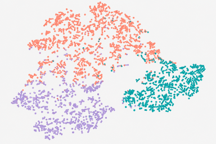
\includegraphics[width=0.45\linewidth]{figure/ACM_clusters.png}
    \caption{t-SNE visualization of learned ACM paper embeddings. Each point represents one paper, and color denotes its class.}
    \label{fig:clustering-acm}
\end{figure}

\begin{figure}[H]
    \centering
    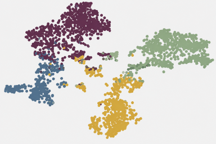
\includegraphics[width=0.45\linewidth]{figure/DBLP_clusters.png}
    \caption{t-SNE visualization of learned DBLP author embeddings. Each point represents one author, and color denotes its research area.}
    \label{fig:clustering-dblp}
\end{figure}

\begin{table}[H]
  \centering
  \caption{Additional clustering-quality diagnostics on DBLP and ACM,
  reported as mean $\pm$ standard deviation over five runs. Best mean
  values are bold.}
  \label{tab:clustering-diagnostic}
  \scriptsize
  \setlength{\tabcolsep}{2.5pt}
  \resizebox{\columnwidth}{!}{%
  \begin{tabular}{llcccc}
    \toprule
    & & \multicolumn{2}{c}{DBLP} & \multicolumn{2}{c}{ACM} \\
    \cmidrule(lr){3-4}
    \cmidrule(lr){5-6}
    \textbf{Group} & \textbf{Model}
    & NMI & ARI
    & NMI & ARI \\
    \midrule

    Hom./hom.
    & GAT
    & $71.50 \pm 0.36$
    & $77.26 \pm 0.48$
    & $57.22 \pm 0.19$
    & $60.47 \pm 0.31$ \\
    \midrule

    \multirow{2}{*}{Het./hom.}
    & NSD
    & $80.21 \pm 0.62$
    & $84.04 \pm 0.43$
    & $62.56 \pm 0.37$
    & $65.02 \pm 0.28$ \\

    & CSNN
    & $81.72 \pm 0.39$
    & $84.25 \pm 0.55$
    & $69.28 \pm 0.45$
    & $71.10 \pm 0.34$ \\
    \midrule

    \multirow{2}{*}{Hom./het.}
    & HAN
    & $79.12 \pm 0.47$
    & $84.76 \pm 0.58$
    & $60.63 \pm 0.22$
    & $64.28 \pm 0.41$ \\

    & PSHGCN
    & $80.38 \pm 0.52$
    & $82.65 \pm 0.36$
    & $71.89 \pm 0.49$
    & $74.31 \pm 0.57$ \\
    \midrule

    \multirow{2}{*}{Het./het.}
    & Hetero2Net
    & $80.54 \pm 0.33$
    & $84.98 \pm 0.46$
    & $70.14 \pm 0.40$
    & $73.42 \pm 0.51$ \\

    & LatGRL
    & $81.36 \pm 0.56$
    & $86.07 \pm 0.38$
    & $72.52 \pm 0.61$
    & $76.75 \pm 0.44$ \\
    \midrule

    Ours
    & \textbf{\method{}}
    & $\mathbf{82.41 \pm 0.35}$
    & $\mathbf{86.52 \pm 0.42}$
    & $\mathbf{75.78 \pm 0.37}$
    & $\mathbf{78.29 \pm 0.31}$ \\
    \bottomrule
  \end{tabular}
  }
\end{table}

\section{Additional Analysis: Diffusion Process of {\method{}}}
\label{sec:diffusion-process-analysis}

We further inspected the training dynamics of \method{} on a controlled four-class
\texttt{FakeHeteroDataset} from torch geometric library. The model was trained with the default synthetic-data settings, and
the visualization includes only nodes with class labels. We recorded the classified-node embedding
layout every five epochs. As shown in Figure~\ref{fig:fakehetero-diffusion-process}, at the beginning of training, nodes from different classes are strongly interleaved. As training proceeds, same-class nodes gradually move toward compact regions, and the
four class-level groups become increasingly separated. This observation suggests that \method{} effectively learns to diffuse information across the heterogeneous graph structure, leading to improved class separability in the learned embeddings.

 \begin{figure}[H]
   \centering
   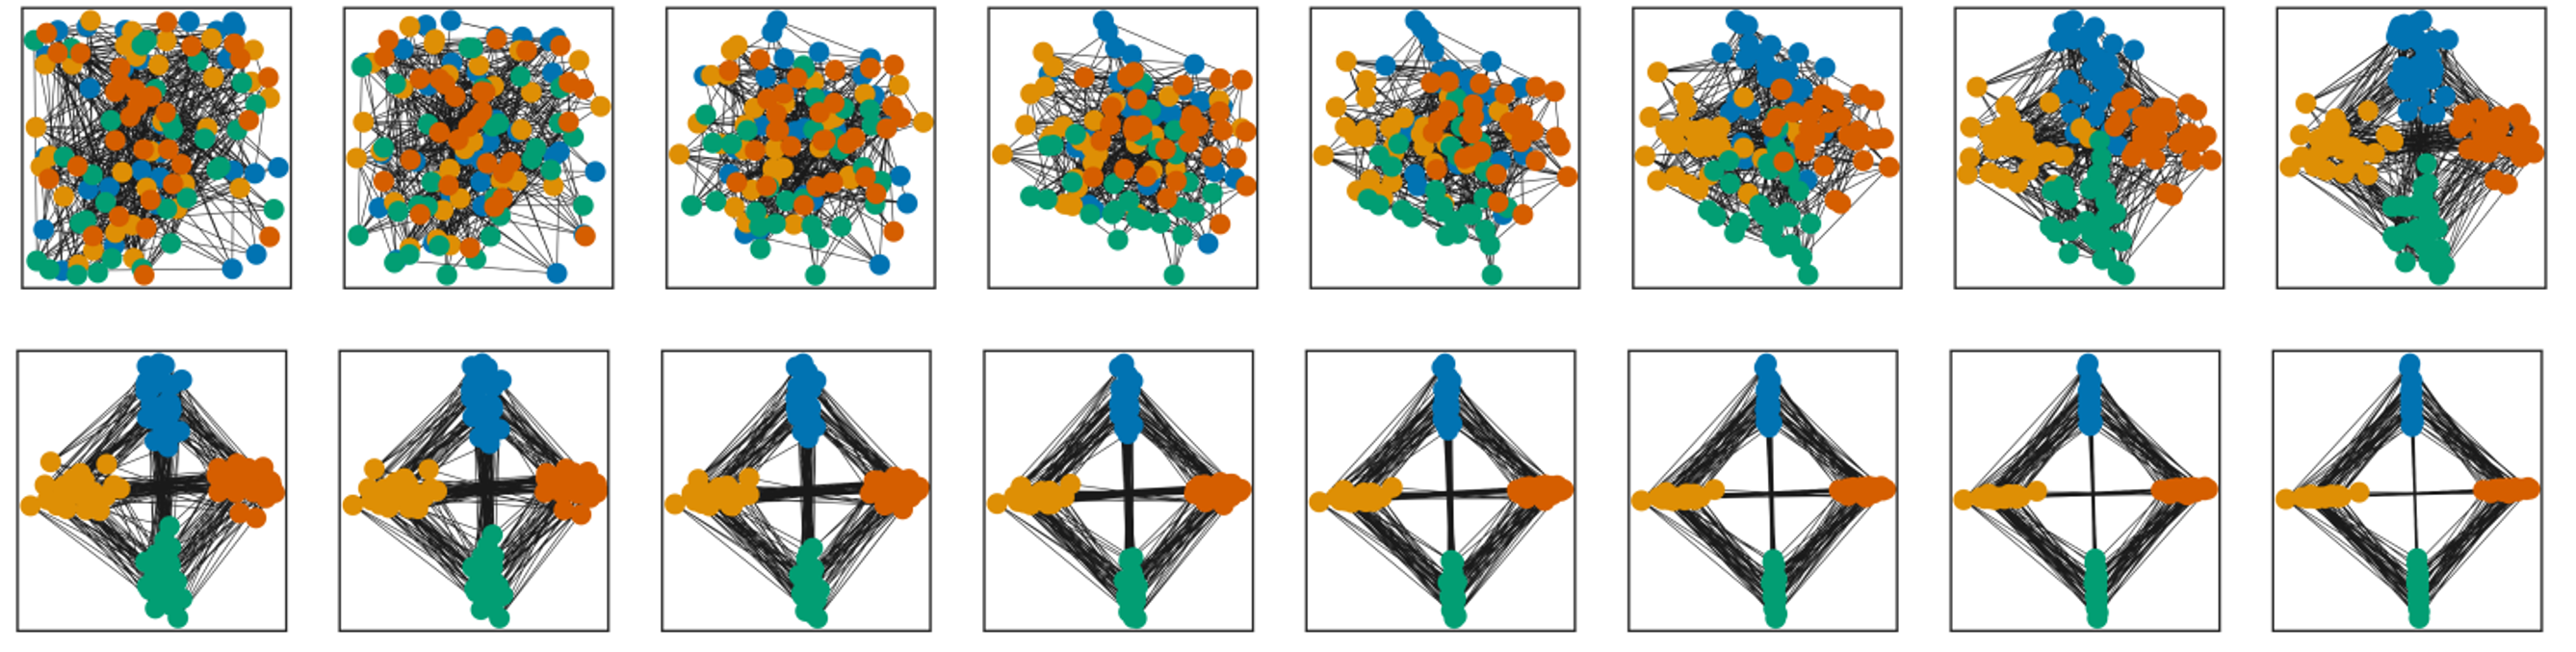
\includegraphics[width=\linewidth]{figure/fakehetero_diffusion_process.png}
   \caption{Training-time diffusion trajectory of \method{} on the four-class
   \texttt{FakeHeteroDataset}. Only labeled nodes are visualized, and consecutive panels are
   separated by five training epochs.}
  \label{fig:fakehetero-diffusion-process}
\end{figure}

\section{Computational Efficiency}

To have a better understanding of the computational cost, we conducted a big-O analysis of \method{}'s, \ampss{}'s, and \sheafcovpool{}'s time and space complexity.

Let $N=|V|$ and
$M=|E|$ be the number of nodes and directed edges, $F$ the number of retained path instances,
and $I=\sum_{f=1}^F \ell_f$ the total edge-face incidences ($\ell_f$ = length of instance
$f$). Let $d$ and $d_r$ denote the stalk and relation-embedding dimensions, and $K$ the number
of Hodge-diffusion steps. Because every edge on a retained path contributes its own edge-to-face
restriction map, the upper Hodge term scales with $I$ rather than $F$ alone.

\paragraph{\ampss{} preprocessing.} Schema construction runs once, before training. With $P$
label-propagation steps, $C_y$ classes, $C_\Sigma$ candidate schemas, $S$ retained schemas,
maximum schema length $L$, and $Q_{\mathrm{type}}$, $Q_{\mathrm{path}}$ the number of typed
and concrete path prefixes visited during enumeration and scoring, preprocessing costs
\[
O\!\left(P(M+N)C_y + Q_{\mathrm{type}} + Q_{\mathrm{path}} + \widehat{F}C_y + C_\Sigma S U + I\right)
\]
time and $O\!\left(M+NC_y+C_\Sigma(L+U)+I\right)$ space, where $\widehat{F}$ instances are
sampled for scoring and $U$ bounds a sampled endpoint set. In the worst case
$Q_{\mathrm{type}}=O(Tb_\Sigma^{L})$ and $Q_{\mathrm{path}}=O((C_\Sigma+S)N\bar{d}^{\,L})$;
in practice \ampss{} caps $C_\Sigma$, $S$, and the number of materialized instances, so the
realized cost is output-sensitive rather than exponential. At inference, the schema gates
cost $O(S)$ per forward pass, and the instance gates (MLP width $h_\beta$) add
$O\!\left(F(2d+d_r)h_\beta\right)$ time and $O(F)$ space.

\paragraph{\method{}.} Table~\ref{tab:complexity} summarizes the per-component
cost of a forward pass, with node-to-edge and edge-to-face MLP widths $h_e$, $h_f$, and
$q(d)=O(d^3)$ for the Householder parameterizations we implement ($O(d^2)$ for
unrestricted dense maps).

\begin{table}[h]
\centering
\scriptsize
\caption{Per-component time and space complexity of the \method{} model. $K$ is the number of diffusion steps}
\label{tab:complexity}
\begin{tabular}{lll}
\toprule
Component & Time & Space \\
\midrule
Node-to-edge & $M\left[(2d+d_r)h_e+h_ed^2+q(d)\right]$ & $Md^2$ \\
Edge-to-face & $(I+F)(d+d_r)h_f+Fh_fd^2$ & $Id^2$ \\
Hodge diffusion & $K(M+I)d^2$ & $(M+I)d^2$ \\
\bottomrule
\end{tabular}
\end{table}

Since node-to-edge and edge-to-face maps are cached and reused across all $K$ diffusion
steps, the full forward pass (excluding readout) costs
\[
O\!\left(Nd_{\mathrm{in}}d + (M+I)d^3 + K(M+I)d^2\right)
\]
once hidden widths scale with $d$, linear in the number of edges and retained edge-face
incidences for fixed $d$. Inference memory is $O\!\left((M+I)d^2+(N+M)d+Fh_f\right)$,
dominated by the cached maps; training adds up to $O(K(N+M)d)$ for the diffusion trajectory.
Note that the edge-to-face encoder holds one hidden vector per path \emph{instance} rather than
one per incidence, since the concatenation in Eq.~\eqref{eq:face-map} collapses the position axis
in its first layer.

\paragraph{\sheafcovpool{} readout.} With $r=3$ node/edge views, projected-descriptor
dimension $f$, pooling width $h_p$, batch size $G$, and $C$ classes, the readout costs
\[
\begin{array}{@{}l@{}}
O\bigl((N+M)[dr^2+r^2h_p+h_pf+f^2] \\
\qquad{}+G[h_pf^2+h_pC]\bigr)
\end{array}
\]
time and
\[
O\!\left((N+M)(dr+f^2)+Gf^2\right)
\]
space. With $r=3$ and $f=8$ fixed, this reduces to $O((N+M)d)$: a linear-time readout
added on top of the model, with no dense Laplacian, node-node covariance, or coarsened graph
ever built.

Furthermore, we reported measured runtime, parameter count, and memory on the ACM node
classification task in Table~\ref{tab:efficiency}.

\begin{table}[H]
  \centering
  \caption{Efficiency comparison on ACM. Best values are bold. Hetsheaf's code is not available, so we used the Hetsheaf-ensemble model reported results in the original paper.}
  \label{tab:efficiency}
  \scriptsize
  \begin{tabular}{lccc}
    \toprule
    \textbf{Model} & Runtime (s) & Parameters & Memory (MB) \\
    \midrule
    R-GCN & \textbf{22.1} & 43M & 1{,}240 \\
    HAN & 28.9 & 2.2M & 1{,}780 \\
    HGT & 1{,}025.8 & 7.2M & 6{,}120 \\
    Sheaf-NSD & 47.6 & \textbf{155K} & \textbf{980} \\
    Hetsheaf & 55.7 & 174K & - \\
    \midrule
    \textbf{\method{}} & 72.1 & 517K & 1120 \\
    \bottomrule
  \end{tabular}
\end{table}

\method{} is not the cheapest model in Table~\ref{tab:efficiency}: R-GCN has the lowest runtime,
and Sheaf-NSD, which models neither relation types nor meta-paths, uses the fewest parameters and
the least memory among the compared models. \method{}'s runtime and parameter count are higher
than Hetsheaf's, the closest heterogeneous sheaf baseline, which we attribute to the additional
edge-to-face maps and \ampss{} schema and instance gates that Hetsheaf does not have. Its memory
footprint nonetheless stays within the same order of magnitude as the other compared models and
well below the heterogeneous transformer baseline HGT, so retaining explicit face-level edge state
does not come at a disproportionate memory cost.

\end{document}
